%
%		LAMA_Implementation_Doc
%
\documentclass[pdftex,a4paper,parskip,listof=totoc,bibliography=totoc,onehalfspacing,12pt]{scrreprt}
\usepackage[english]{babel} % If german is needed add ngerman in first bracket 
\usepackage[utf8]{inputenc}
\usepackage[T1]{fontenc}
\usepackage{lmodern}
\usepackage{textcomp}
\usepackage{multirow}
%\usepackage{graphicx} is loaded with pdfpages
\usepackage{pict2e}
\usepackage{multicol}
\usepackage[automark]{scrpage2}
\usepackage{setspace}
\usepackage{color}
\usepackage{natbib}
\usepackage{booktabs}
\usepackage{amsmath}
\usepackage{mathtools}			%For use of \mathrlap and \mathllap
\usepackage{amsfonts}			%For use of \mathbb{R} (e.g. show real number letter)
\usepackage{float}
\usepackage{longtable}
\usepackage{pdfpages}
\usepackage{eso-pic}
\usepackage{dirtree}
\usepackage{multirow}
\usepackage{gauss}				% For use of \newcommand*\dashline... (vertical line in arrays)
\usepackage[vlined]{algorithm2e}
\usepackage{enumitem}
	\setlist[itemize]{itemsep=-12pt}
	\setlist[enumerate]{itemsep=-12pt}
\usepackage{subcaption}
\usepackage{lscape}		%For use of \begin{landscape} \end{landscape} Zur Darstellung einzelner Seiten im Querformat
\usepackage{adjustbox}
\usepackage{nicefrac}
\usepackage{physics}
%\usepackage{underscore}
\KOMAoptions{twoside}
\setcounter{MaxMatrixCols}{50}

\usepackage[left=25mm,right=25mm,bottom=35mm, footskip=20mm]{geometry}

\usepackage{siunitx}		% Show units
\sisetup{per-mode=fraction}	% Representation of fractions

\usepackage{listings}
\usepackage{scrhack}		% Comma-option \KOMAoption{listof}{leveldown} only effects lstlistoflistings 

\lstdefinestyle{MyMatlab}		% Definition of individual listing-styles
{						% Applications with "\lstinputlisting[style=MyMatlab]{../reflexion/Matlab_Skripte/resample.m}"
	language={Matlab},
	captionpos={t},
	inputencoding={latin1},
	showstringspaces={false},
	frame={tlRB},
	basicstyle=\scriptsize
}

\lstdefinestyle{MyC++}
{
	language={C++},
	tabsize={8},
	captionpos={t},
	frame={tlRB},
	basicstyle=\tiny
}

\lstdefinestyle{MyFortran}
{
	language={[77]Fortran},
	captionpos={t},
	frame={tlRB},
	basicstyle=\tiny
}

\lstdefinestyle{MySh}
{
	language={sh},
	captionpos={t},
	frame={tlRB},
	basicstyle=\tiny
}

\lstdefinestyle{MyGnuplot}
{
	language={Gnuplot},
	captionpos={t},
	frame={tlRB},
	basicstyle=\scriptsize
}

\lstset{literate=%
  {Ö}{{\"O}}1
  {Ä}{{\"A}}1
  {Ü}{{\"U}}1
  {ß}{{\ss}}2
  {ü}{{\"u}}1
  {ä}{{\"a}}1
  {ö}{{\"o}}1
}

\usepackage{rotating}
\usepackage{wrapfig}
\usepackage{tikz}
	\usetikzlibrary{shapes}
	\usetikzlibrary{decorations.pathmorphing}
	\usetikzlibrary{decorations.shapes}
	\usetikzlibrary{shapes.geometric}
	\pgfdeclarelayer{edgelayer}
	\pgfdeclarelayer{nodelayer}
	\pgfsetlayers{edgelayer,nodelayer,main}
	\tikzstyle{none}=[inner sep=0pt]
	\tikzset{decorate with/.style={decorate,decoration={shape backgrounds,shape=#1,shape size=2mm}}}

\definecolor{blue}{rgb}{0.01,0.01,0.95}	%HEX: 0202F2
\definecolor{green}{rgb}{0.01,0.65,0.01}	%HEX: 02A602
\definecolor{red}{rgb}{0.95,0.01,0.01}	%HEX: F20202
\definecolor{brown}{rgb}{0.55,0.27,0.07}	%HEX: 8B4513
\definecolor{violet}{rgb}{0.65,0.05,0.7}	%HEX: A60DB3

\setcounter{tocdepth}{1}	%Legt die Anzeigetiefe des Inhaltsverzeichnisses fest

\renewcommand{\theequation}{\arabic{section}.\arabic{equation}} %Die Nummerierung Formeln wird geändert

\renewcommand{\partheadmidvskip}{\enskip}
\renewcommand{\partformat}{\thepart\autodot}

\renewcommand{\arraystretch}{1.2} %Legt den Faktor fest, um den der Zeilenabstand innerhalb einer Tabelle oder eines Array gedeht wird
\newcommand*\dashline{\hspace{-0.3em}\rotatebox[origin=c]{90}{\scalebox{-0.3}[1]{$-~~-$}}\hspace{-0.3em}}
\newcommand*\longdashline{\hspace{-0.3em}\rotatebox[origin=c]{90}{\scalebox{-0.4}[1]{$-~~-~~-~~-$}}\hspace{-0.3em}}

%\setlength{\oddsidemargin}{20mm} 
%\setlength{\evensidemargin}{20mm} 

\renewcommand*{\chapterheadstartvskip}{\vspace*{-1\baselineskip}}	%legt Abstand vor chapter fest

\newcommand{\CC}[1][]{$\text{C\hspace{0ex}}^{_{_{_{++}}}}					%Write nicer ++ signs in C++
                      \ifthenelse{\equal{#1}{}}{}{\text{\hspace{-.625ex}#1}}$} 
\newcommand{\clang}[1][]{$\text{clang\hspace{0ex}}^{_{_{_{++}}}}		%Write nicer ++ signs in clang++
                      \ifthenelse{\equal{#1}{}}{}{\text{\hspace{-.25ex}(#1)}}$} 
\newcommand{\gCC}[1][]{$\text{g\hspace{0ex}}^{_{_{_{++}}}}				%Write nicer ++ signs in g++
                      \ifthenelse{\equal{#1}{}}{}{\text{\hspace{-.25ex}(#1)}}$} 
                      
\newcommand\coolover[2]{\mathrlap{\smash{%
\overbrace{\phantom{\begin{matrix} #2 %
\end{matrix}}}^{\mbox{$#1$}}}}#2}
                      
\newcommand{\shellcmd}[1]{\indent\indent\texttt{#1}}	%change font for shell entries  
\newcommand{\shellcmdline}[1]{\indent\indent\texttt{\quad#1}} 	%change font for command lines and indention

\makeatother
\usepackage{hyperref}
\definecolor{LinkColor}{rgb}{0,0,0.75}
\hypersetup{                    %Farben der Links im pdf werden festgelegt
colorlinks=true,
linkcolor=LinkColor,
citecolor=LinkColor,
filecolor=LinkColor,
menucolor=LinkColor,
pagecolor=LinkColor,
urlcolor=LinkColor}

\KOMAoption{listof}{leveldown} %Bewirkt, dass listoffigures, listoftables und lstlistoflistings nicht als chapter behandelt werden. Erschenungsbild im Inhaltsverzeichnis und im Dokument selbst (kein automatischer seitenumbruch am Ende der Verzeichnisse).

\pagestyle{scrheadings} %Legt die Art des Seitenformats für alle folgenden Seiten fest. scrheadings: Um bei zweiseitig formatierten Dokumenten (=Bücher, die unterschiedliche "`linke"' und "`rechte"' Seiten haben) den Seitenkopf und -fuß automatisch an die jeweilige Seite anzupassen, gibt es die folgenden Befehle: \ihead, \chead, \ohead, \ifoot, \cfoot, \ofoot für scrheadings wird "`\usepackage{scrpage2}"' benötigt
\clearscrheadfoot %Löscht alle Kopf- und Fußzeilen
\ohead{\headmark}
\automark[section]{chapter}
\ofoot[\pagemark]{\pagemark}		%[plain-Seiten]{normale Seiten}
\setheadsepline{0.4pt} %erzeugt eine Linie der Stärke 0.4pt zwischen Rumpf und Kopfzeile
\setlength{\headsep}{10mm} %Legt den Abstand zwischen der Kopfzeile und dem Rumpf der Seite fest

\hyphenation{CATIA} %definiert die Stellen zum Trennen von Wörter mit "`-"' Beispiel: \hyphenation{er-go-no-mic}

\title{LAMA_Implementation_Doc}
\author{}
\graphicspath{{@CMAKE_SOURCE_DIR@/../doc/guide/}}

\begin{document}

\selectlanguage{english}

\numberwithin{equation}{chapter} %legt die Formelnummerierung fest

\thispagestyle{empty} %Kopf und Fußzeile wird für diese Seite ausgeschaltet
\newgeometry{left=25mm,right=25mm,bottom=40mm,top=20mm}
\begin{figure}[h] % Gleiten ist durch Verwendung des H verhindert
\begin{flushright}

\includegraphics[scale=0.15]{./images/wave_logo.png}
\end{flushright}
\end{figure}

\begin{center}
\vspace{2cm}
\huge{WAVE-Simulation }\\
\vspace{0.5cm}
\large{HPC Finite Difference Simulation in Matrix-Vector Formalism}
\end{center}

\vfill
\begin{center}
{\Large{\url{wave-toolbox.org}}}

{\small Document created \today}
\end{center}

\newpage 
\thispagestyle{empty}
\begin{center}
{\large
Supported by the German Ministry of Education and Research (BMBF) through the project \textbf{WAVE}, grant 01IH15004A.
}
\end{center}

\cleardoublepage

\pagenumbering{Roman}
\setcounter{page}{1}
\restoregeometry

\newpage

\tableofcontents % Table of contents is inserted \tableofcontens (insert \addcontentsline, so the content is linked correctly)
\addcontentsline{toc}{chapter}{Contents} %"Contents" will be displayed in contents

\pagenumbering{arabic}
\setcounter{page}{1}

\cleardoublepage
%\markboth{}{License}
\chapter*{License}
\addcontentsline{toc}{chapter}{License}

WAVE-Simulation is free software: you can redistribute it and/or modify it under the terms of the GNU Affero General Public License (GNU AGPL v3) as published by the Free Software Foundation, version 3.0 of the License only.
 
WAVE-Simulation is distributed in the hope that it will be useful, but WITHOUT ANY WARRANTY; without even the implied warranty of MERCHANTABILITY or FITNESS FOR A PARTICULAR PURPOSE. See the GNU Affero General Public License for more details. You should have received a copy of the GNU Affero General Public License along with Simulation. See file LICENSE and/or \url{https://www.gnu.org/licenses/agpl-3.0.de.html}.

The authors of WAVE-Simulation are listed in file \lstinline{AUTHORS}.

\cleardoublepage
\chapter*{Introduction}
\addcontentsline{toc}{chapter}{Introduction}

In order to extract information about the structure and composition of the crust from seismic observations and ground penetrating radar (GPR) observations, it is necessary to be able to predict how seismic wavefields and electromagnetic (EM) wavefields are affected by complex structures. Since exact analytical solutions to the wave equations do not exist for most subsurface configurations, the solutions can be obtained only by numerical methods. For iterative calculations of synthetic seismograms with limited computer resources fast and accurate modeling methods are needed. The explicit time-domain finite-difference (FD) modeling program WAVE-Simulation (C++), that is described in this guide, is based on the FD approach described by \cite{yee1966numerical}, \cite{virieux1986p} and \cite{levander1988fourth}. To solve a large number of forward problem based on wave equations, modern seismic imaging methods often require high performance computing (HPC) systems to provide enough computational power. In order to parallelise the computation, the problem is rewritten in matrix-vector formulation. By using matrix-vector formulation the parallelisation problem can be outsourced using a HPC-framework. In our case WAVE-Simulation uses the open source framework LAMA which is a HPC library enabling the development of hardware independent Software executable on both CPUs and GPUs.

WAVE-Simulation features solving seismic waves and EM waves by utilising an explicit time-domain FD method. Seismic waves include the acoustic, elastic and viscoelastic wave equation in 2D and 3D and Shear Horizontal (SH) wave in 2D, while EM waves include (visco) transverse magnetic (TM) mode and (visco) transverse electric (TE) mode in 2D and visco-EM wave in 3D. The current version of WAVE-Simulation also includes the extension of higher order FD operators and applying Perfectly Matched Layer boundary conditions at the edges of the numerical mesh \citep{berenger1994perfectly,roden2000convolution,komatitsch2007unsplit}. It also includes the stress-image method by \cite{levander1988fourth} and the improved vacuum formulation by \cite{zeng2012improved} for modelling the free surface in seismic wave propagation. 

In the following sections, by taking 3D elastic wave equation as an example, we give a short description of the theoretical background, the different modelling parameters and options and how the program is used and executed. The others such as the acoustic, viscoelastic, EM and visco-EM wave equations are shown in the appendix \ref{sec:Acoustic_wave_equation}-\ref{sec:Visco_EM_wave_equation}.

\cleardoublepage
\part{Theory of Finite Difference Simulation in Matrix-Vector Formalism}

\chapter{Physical Derivation of Seismic Wave Propagations}

This chapter contains the theoretical principles for the physical description of seismic wave propagation in elastic media. This also includes the general stress-stain relation of solid objects or viscous fluids. Furthermore conservation of momentum is applied to infinitesimal volume elements.

\section{General State of Stress}
\label{sec:AllSp}

Other than not viscous fluids, viscous fluids and solid objects can be under shear stress. The normal stress in all spatial directions is generally varying. This can be explained by internal friction.

The state of stress is represented by an infinitesimal volume element  $\partial V = \partial x~ \partial y~ \partial z$, as shown in figure \ref{fig:AllgSpZu}.
In index notation $\sigma_{ij}$, index $i$ represents the direction of the surface normal, which is affected by the stress and index $j$ describes the direction of the stress itself. $\sigma_{ii}$ correspond to normal stress with the convention $\sigma_{ii} > 0$: tension and $\sigma_{ii} < 0$: compression. $\sigma_{ij}$ with  $i \neq j$ are also denoted by $\tau_{ij}$ and correspond to shear stress. 
\begin{figure}
\centering
\begin{tikzpicture}
	\begin{pgfonlayer}{nodelayer}
		\node [style=none] (0) at (0, 0) {};
		\node [style=none, label=-180:$x$] (1) at (-1, -1) {};
		\node [style=none, label=-90:$y$] (2) at (2, 0) {};
		\node [style=none, label=-180:$z$] (3) at (0, 2) {};
		\node [style=none] (4) at (5, 0) {};
		\node [style=none] (5) at (3, -2) {};
		\node [style=none] (6) at (9, 0) {};
		\node [style=none] (7) at (7, -2) {};
		\node [style=none] (8) at (5, 4) {};
		\node [style=none] (9) at (9, 4) {};
		\node [style=none] (10) at (3, 2) {};
		\node [style=none] (11) at (7, 2) {};
		\node [style=none, label=-90:\textcolor{red}{$\tau_{12}$}] (12) at (6, 0) {};
		\node [style=none, label=-180:\textcolor{red}{$\tau_{13}$}] (13) at (5, 1) {};
		\node [style=none, label=180:\textcolor{green}{$\sigma_{11}$}] (14) at (4.5, -0.5) {};
		\node [style=none] (15) at (8, 1) {};
		\node [style=none, label=-180:\textcolor{red}{$\tau_{23}$}] (16) at (8, 2) {};
		\node [style=none, label=0:\textcolor{red}{$\tau_{21}$}] (17) at (7.5, 0.5) {};
		\node [style=none, label=-135:\textcolor{green}{$\sigma_{22}$}] (18) at (9, 1) {};
		\node [style=none] (19) at (6, 3) {};
		\node [style=none, label=-180:\textcolor{red}{$\tau_{31}$}] (20) at (5.5, 2.5) {};
		\node [style=none, label=-90:\textcolor{red}{$\tau_{32}$}] (21) at (7, 3) {};
		\node [style=none, label=-135:\textcolor{green}{$\sigma_{33}$}] (22) at (6, 4) {};
	\end{pgfonlayer}
	\begin{pgfonlayer}{edgelayer}
		\draw [->] (0.center) to (1.center);
		\draw [->] (0.center) to (2.center);
		\draw [->] (0.center) to (3.center);
		\draw [line width = 1.2](8.center) to (10.center);
		\draw [line width = 1.2](10.center) to (5.center);
		\draw [line width = 1.2](5.center) to (7.center);
		\draw [line width = 1.2](7.center) to (6.center);
		\draw [line width = 1.2](6.center) to (9.center);
		\draw [line width = 1.2](8.center) to (9.center);
		\draw [line width = 1.2](10.center) to (11.center);
		\draw [line width = 1.2](11.center) to (9.center);
		\draw [line width = 1.2](11.center) to (7.center);
		\draw [->, color=red] (4.center) to (12.center);
		\draw [->, color=green] (4.center) to (14.center);
		\draw [->, color=red] (4.center) to (13.center);
		\draw [->, color=red] (15.center) to (17.center);
		\draw [->, color=red] (15.center) to (16.center);
		\draw [->, color=green] (15.center) to (18.center);
		\draw [->, color=red] (19.center) to (20.center);
		\draw [->, color=red] (19.center) to (21.center);
		\draw [->, color=green] (19.center) to (22.center);
	\end{pgfonlayer}
\end{tikzpicture}
\caption[Representation of the general stress state by a volume element.]{Representation of the general stress state by a volume element $\partial V = \partial x~ \partial y~ \partial z$. Where $\sigma_{ij}$ corresponds to normal stress and $\tau_{ij}$ to shear stress. }
\label{fig:AllgSpZu}
\end{figure}

As the state of stress represents an object in a static equilibrium, for every tension on one of the three covered sides there exists a counter-stress in the opposite direction. 

\begin{minipage}[t]{0.4\textwidth}
\begin{equation}
	\sigma_{ij}=\left(
\begin{array}{ccc}
\sigma_{11} & \tau_{12} & \tau_{13}\\
\tau_{21} & \sigma_{22} & \tau_{23}\\
\tau_{31} & \tau_{32} & \sigma_{33}
\end{array}
\right)
\end{equation}
\end{minipage}
\hfill
\begin{minipage}[t]{0.45\textwidth}
To prevent the volume from rotation the following must apply: $\sigma_{ij} = \sigma_{ji}$ (conservation of angular momentum). Hence, $\sigma_{ij}$ is symmetric and contains \num{6} independent entries of stress.
\end{minipage}

By applying Hook's law a connection between stress and dilatation  can be established. In case of small dilatations in comparison to the wavelength, which in case of seismic waves is always given, the dependancy of the stress component to dilatation can be approximated as a linear relation.
\begin{minipage}[t]{0.4\textwidth}
\begin{equation}
	\sigma_{ij} = C_{ijkl} \cdot\epsilon_{kl}
\end{equation}
\end{minipage}
\hfill
\begin{minipage}[t]{0.45\textwidth}
$\sigma_{ij}$: stress tensor\\
$\epsilon_{kl}$: strain tensor\\
$C_{ijkl}$: stiffness tensor
\end{minipage}
The stiffness tensor $C_{ijkl}$ is \num{4}-dimensional and in general has $3^4 = 81$ elements. Because $\sigma_{ij}$ and $\epsilon_{kl}$ are symmetrical, the number of independent components reduces to \num{36}. With energetic reasoning the problem can be reduced furthermore to \num{21} and in isotropic media eventually even to \num{2} components. 

Thus the generalised Hook's law for linear elastic and isotropic media can be derived:
\begin{align}
	\sigma_{ij} &= \lambda \theta \delta_{ij} + 2 \mu \epsilon_{ij}\label{eqn:GenHook}\\
	\epsilon_{ij} &= \frac{1}{2} \left( \frac{\partial u_i}{\partial x_j} + \frac{\partial u_j}{\partial x_i} \right)\label{eqn:Dehnij}
\end{align}
Here $\lambda$ is the second Lam\'{e} parameter and $\mu$ the second Lam\'{e} parameter. $\delta_{ij}$ is equivalent to the Kronecker delta. $\theta=\epsilon_{11} + \epsilon_{22} + \epsilon_{33}$ is the cubic dilatation. $\epsilon_{ij}$ represents the linear strain tensor and $u_i$ resembles the displacement of a particle in $i$-direction.

\section{Conservation of Momentum}

Beside the stress-stain relation, conservation of momentum is main a core concept for elastic seismic wave propagation. In principle conservation of momentum corresponds to differential formulation of a dynamic equilibrium per volume unit. There are two applying force to an infinitesimal volume with edge length $\partial x_i$, volume force and surface force. \citep{landau1997lehrbuch}.

Volume force, inertial force and gravitational force apply to objects due to having mass. 
Inertial forces can be derived by applying Newton's  second law of motion in it's original formulation: 
\begin{equation}
	\frac{\mathrm{d} p}{\mathrm{d} t} = \frac{\mathrm{d} (\partial m \cdot v_i)}{\mathrm{d} t} = \underbrace{\frac{\mathrm{d} (\partial m)}{\mathrm{d} t}}_{\mathrlap{\text{$= 0$ , as $m$ is $t$-independent}}} v_i + \partial m \frac{\mathrm{d} v_i}{\mathrm{d} t}
\end{equation}
Writing the inertial force density with $v_i = v_i (x_k,t)$:
\begin{equation}
	f_{I,i} = \frac{\partial m}{\partial V} \frac{\mathrm{d} v_i}{\mathrm{d} t} = \rho \frac{\mathrm{d} v_i}{\mathrm{d} t} = \rho \bigg[ \frac{\partial v_i}{\partial t} + \underbrace{v_k \frac{\partial v_i}{\partial x_k}}_{\mathrlap{\substack{\text{$\approx 0$, for small shifts in relation}\\\text{ to the wavelength}}}} \bigg] \approx \rho \frac{\partial v_i}{\partial t}\label{eqn:TKD}
\end{equation}
For elastic body waves, the gravitational force can be ignored. Only in case of low frequent natural oscillation, gravitation has an effect and should be considered.

Surface forces affect an object due to its stress conditions. The derivation of surface forces is made by evaluating the force balance in all three spatial directions. To begin with the surface force can be written as an integration of the stress vector $\vec{s}$ over the object's surface $\partial A$.
\begin{equation}
	\vec{F}_s = \int_A \vec{s} ~\mathrm{d}A
\end{equation}
In general the stress vector, perpendicular to an arbitrary surface, can be calculated by multiplying the transposed stress tensor with the normal vector of the surface $\vec{n}$. Note that the stress tensor is symmetric due to conservation of angular momentum (see chapter \ref{sec:AllSp}) and therefore $\sigma^T = \sigma$ applies.
\begin{equation}
	\vec{s} = \sigma^\mathrm{T} \cdot\vec{n}
\end{equation}
With a directed plane element $\mathrm{d}\vec{A} = \vec{n} ~\mathrm{d}A$, the surface force can be rewritten to: 
\begin{equation}
	\vec{F}_s = \int_A \sigma \cdot\vec{n} ~\mathrm{d}A = \int_A \sigma \mathrm{d}\vec{A} 
\end{equation}
The divergence theorem also known as Gauss's theorem $\int_A \vec{F}~\mathrm{d}\vec{A} = \int_V \operatorname{div} \vec{F} ~\mathrm{d}V$ enable to transfer the surface integral to a volume integral. This is beneficial to obtain the surface force density $\vec{f}_{s}$, by simply dividing the surface force by the volume. 
\begin{align}
	\vec{F}_s &= \int_A \sigma \mathrm{d}\vec{A} = \int_V \operatorname{div} \sigma ~\mathrm{d}V\\
	\vec{f}_s &= \frac{\vec{F}_s}{\mathrm{d}V} = \operatorname{div} \sigma~~~~~~~\vec{f}_{s,i} = \frac{\partial \sigma_{ij}}{\partial x_j}\label{eqn:OFKD}
\end{align}
Finally the equilibrium of forces $f_{T,i} = f_{s,i}$, resulting from equation \ref{eqn:TKD} and \ref{eqn:OFKD} can be formulated to obtain the equation of motion 
\begin{equation}
	\rho \frac{\partial v_i}{\partial t} =  \frac{\partial \sigma_{ji}}{\partial x_j}\label{eqn:ElBewGl}
\end{equation}
The three equations \ref{eqn:ElBewGl}, \ref{eqn:GenHook} and \ref{eqn:Dehnij} describe a complete seismic wave propagation in linear elastic and isotropic media. Time-derivation of equations \ref{eqn:GenHook} and \ref{eqn:Dehnij} together with equation \ref{eqn:ElBewGl} leads to the stress-velocity formulation:
\begin{align}
	\frac{\partial\sigma_{ij}}{\partial t} &= \lambda \frac{\partial \theta}{\partial t} \delta_{ij} + 2 \mu \frac{\partial \epsilon_{ij}}{\partial t}\label{eqn:GenHookdt}\\
	\frac{\partial \theta}{\partial t} &= \frac{\partial v_1}{\partial x_1} + \frac{\partial v_2}{\partial x_2} + \frac{\partial v_3}{\partial x_3} = \frac{\partial v_k}{\partial x_k} \\
	\frac{\partial\epsilon_{ij}}{\partial t} &= \frac{1}{2} \left( \frac{\partial v_i}{\partial x_j} + \frac{\partial v_j}{\partial x_i} \right)\label{eqn:Dehnijdt}
\end{align}
\cleardoublepage

\chapter{Discretization}

To solve the wave equations with finite differences, the physical continuous space and time have to be discretised in mathematical grids. Space and time coordinates are given by $x=i \cdot \Delta x$, $y=j \cdot \Delta y$, $z=k \cdot \Delta z$ and $t=n \cdot \Delta t$. The spacial intervals between grid points in each direction are represented by $\Delta x, \Delta y$ and $\Delta z$. $\Delta t$ is equivalent to a time interval. The total grid size $N$ is equal to $NX \times NY \times NZ$ and the simulation duration $T$ is $NT \cdot \Delta t$.

\section{Definition of the \textit{Standard Staggered Grid} (SSG)} \label{sec:SSG}

The \textit{Standard Staggered Grid} (SSG) \citep{virieux1986p,levander1988fourth} is a method to distribute physical quantities over grid points, such that the partial differential wave equations each refer to a common grid point. The shape of the SSG in 3D \citep{graves1996simulating} is shown in figure \ref{fig:StagGrid3D}. Here the temporal dimension is not shown explicitly. Stress components $\sigma_{ij}$ are temporally located on half-spaced grid points, the particle velocity $v_{i}$ is temporally located on full grid points.
\begin{figure}
\begin{tikzpicture} 
    \begin{pgfonlayer}{nodelayer}
	\node [style=none, rectangle, color=green, minimum size=3 mm, fill=green, draw, label=90:{$i,j,k$}, label={[align=left]-70:$\nwarrow p, \sigma_{xx},\sigma_{yy},\sigma_{zz}$\\$\lambda, \mu, \rho,r_{xxl},r_{yyl},r_{zzl}$\\$\tau^p, \tau^s$}] (0) at (0, 0) {};
	\node [style=none, circle, color=orange, minimum size=3 mm, fill=orange, draw, label=90:{$k+\frac{1}{2}$}, label={[align=left]-45:$v_z, \rho_z$}] (1) at (2, 1) {};
	\node [style=none, diamond, color=brown, minimum size=4 mm, fill=brown, draw, label=90:{$i+\frac{1}{2}$}, label={[align=left]-45:$v_x, \rho_x$}] (2) at (4, 0) {};
	\node [style=none, regular polygon,regular polygon sides=5, color=black, minimum size=4 mm, fill=white,line width=0.5 mm, draw, label=90:{$i+\frac{1}{2}, k+\frac{1}{2}$}, label={[align=left]0:$\sigma_{xz}, \mu_{xz}$ \\ $r_{xzl}, \tau^s_{xz}$}] (3) at (6, 1) {};
	\node [style=none,label=0:$z(k)$] (4) at (3, 1.5) {};
	\node [style=none, regular polygon,regular polygon sides=3, color=red, minimum size=4 mm, fill=red, line width=0.5 mm, draw, label=80:{$j+\frac{1}{2}$}, label={[align=left]-45:$v_y, \rho_y$}] (5) at (0, -4) {};
	\node [style=none, rectangle, color=violet, minimum size=3 mm, line width=0.5 mm, fill=white, draw, label=0:{$i+\frac{1}{2}, j+\frac{1}{2}$}, label={[align=left]-90:$\sigma_{xy}, \mu_{xy}$ \\ $r_{xyl}, \tau^s_{xy}$}] (6) at (4, -4) {};
	\node [style=none, regular polygon,regular polygon sides=3, color=blue, minimum size=4 mm, line width=0.5 mm, fill=white, draw, label=-45:{$j+\frac{1}{2}, k+\frac{1}{2}$}, label={[align=left]45:$\sigma_{yz}, \mu_{yz}$ \\ $\swarrow r_{yzl}, \tau^s_{yz}$}] (7) at (2, -3) {};
	\node [style=none] (8) at (6, -3) {};
	\node [style=none,label=-90:$x(i)$] (9) at (7, 0) {};
	\node [style=none,label=0:$y(j)$] (10) at (0, -6) {};	
	\node [style=none,label={[align=right]0:$\mathbf{Acoustic}$ \\ $\mathbf{Viscoelastic}$}] (101) at (4.5, -5.5) {};		
    \end{pgfonlayer}
    \begin{pgfonlayer}{edgelayer}
	\draw (0.center) to (1.center);
	\draw (2.center) to (3.center);
	\draw (0.center) to (2.center);
	\draw (1.center) to (3.center);
	\draw (0.center) to (5.center);
	\draw (5.center) to (6.center);
	\draw [dashed](5.center) to (7.center);
	\draw (6.center) to (8.center);
	\draw [dashed](7.center) to (8.center);
	\draw (6.center) to (2.center);
	\draw [dashed](7.center) to (1.center);
	\draw (8.center) to (3.center);
	\draw [->] (1.center) to (4.center);
	\draw [->] (2.center) to (9.center);
	\draw [->] (5.center) to (10.center);
    \end{pgfonlayer}
    \begin{pgfonlayer}{nodelayer}
	\node [style=none, label=-45:{$i,j,k$}] (11) at (0+8.3, 0) {};
	\node [style=none, circle, color=orange, minimum size=3 mm, fill=orange, draw, label=-9:{$k+\frac{1}{2}$}, label={[align=left]93:$E_z,\varepsilon_{z},\sigma_{ez}$\\$r_{zl},\tau_{\varepsilon z l},\tau_{\sigma e z}$}] (12) at (2+8.3, 1) {};
	\node [style=none, diamond, color=brown, minimum size=4 mm, fill=brown, draw, label=-135:{$i+\frac{1}{2}$}, label={[align=left]-87:$E_x, \varepsilon_{x}, \sigma_{ex}$\\$r_{xl},\tau_{\varepsilon x l},\tau_{\sigma e x}$}] (13) at (4+8.3, 0) {};
	\node [style=none, regular polygon,regular polygon sides=5, color=black, minimum size=4 mm, fill=white,line width=0.5 mm, draw, label=90:{$i+\frac{1}{2}, k+\frac{1}{2}$}, label=-70:{$H_y, \mu_{mxz}$}] (14) at (6+8.3, 1) {};
	\node [style=none,label=0:$z(k)$] (15) at (3+8.3, 1.5) {};
	\node [style=none, regular polygon,regular polygon sides=3, color=red, minimum size=4 mm, fill=red, line width=0.5 mm, draw, label=80:{$j+\frac{1}{2}$}, label={[align=left]-45:$E_y, \varepsilon_{y}, \sigma_{ey}$\\$r_{yl},\tau_{\varepsilon y l},\tau_{\sigma e y}$}] (16) at (0+8.3, -4) {};
	\node [style=none, rectangle, color=violet, minimum size=3 mm, line width=0.5 mm, fill=white, draw, label=0:{$i+\frac{1}{2}, j+\frac{1}{2}$}, label=-90:{$H_z, \mu_{mxy}$}] (17) at (4+8.3, -4) {};
	\node [style=none, regular polygon,regular polygon sides=3, color=blue, minimum size=4 mm, line width=0.5 mm, fill=white, draw, label=45:{$j+\frac{1}{2}, k+\frac{1}{2}$}, label={[align=left]135:$H_x, \mu_{myz}$}] (18) at (2+8.3, -3) {};
	\node [style=none] (19) at (6+8.3, -3) {};
	\node [style=none,label=-90:$x(i)$] (20) at (7+8.3, 0) {};
	\node [style=none,label=0:$y(j)$] (21) at (0+8.3, -6) {};	
	\node [style=none,label=0:$\mathbf{Visco-EM}$] (102) at (4.5+8.3, -5.5) {};		
    \end{pgfonlayer}
    \begin{pgfonlayer}{edgelayer}
	\draw (11.center) to (12.center);
	\draw (13.center) to (14.center);
	\draw (11.center) to (13.center);
	\draw (12.center) to (14.center);
	\draw (11.center) to (16.center);
	\draw (16.center) to (17.center);
	\draw [dashed](16.center) to (18.center);
	\draw (17.center) to (19.center);
	\draw [dashed](18.center) to (19.center);
	\draw (17.center) to (13.center);
	\draw [dashed](18.center) to (12.center);
	\draw (19.center) to (14.center);
	\draw [->] (12.center) to (15.center);
	\draw [->] (13.center) to (20.center);
	\draw [->] (16.center) to (21.center);
    \end{pgfonlayer}
\end{tikzpicture}
\caption[]{Representation of the SSG with the distribution of material and wavefield parameter of acoustic and viscoelastic wave \citep{graves1996simulating} and visco-EM wave \citep{yee1966numerical} in 3D. The seismic wavefields include one pressure value $p$ (only for acoustic wave), six stress values $\sigma_{xx}, \sigma_{yy}, \sigma_{zz}, \sigma_{xy}, \sigma_{xz}, \sigma_{yz}$ and corresponding $6L$ memory variables $r_{xxl}, r_{yyl}, r_{zzl}, r_{xyl}, r_{xzl}, r_{yzl}$ ($l=1,...,L$), three components of particle velocity $v_x, v_y, v_z$. The seismic material parameters include $\lambda, \mu, \tau^p, \tau^s, \rho$. The visco-EM wavefields include three components of electric fields $E_x, E_y, E_z$ and corresponding $3L$ memory variables $r_{xl}, r_{yl}, r_{zl}$ ($l=1,...,L$), three components of magnetic fields $H_x, H_y, H_z$. The visco-EM material parameters include $\mu_m, \varepsilon, \sigma_e, \tau_{\varepsilon l}, \tau_{\sigma e}$. The seismic and visco-EM material parameters $\mathbf{m}$ are located at the integer points or averaged by $i$-direction ($\mathbf{m}_i$) or averaged by $ij$-plane ($\mathbf{m}_{ij}$).}
\label{fig:StagGrid3D}
\end{figure}

Using the solution approach of finite differences, the analytical calculations of spatial and time derivation are approximated by calculating the weighted average (FD-operators) of surrounding grid points. Depending on the FD-operator order, more surrounding grid points are included in the averaging. Models can be approximated more exactly by using higher orders, at the expense of higher computing effort and thus higher computing time.

To accomplish a feasible implementation of the finite difference calculations to solve the wave equations, calculations are made in recursive time-stepping. Therefore, time derivatives of stress and particle velocity are replaced by second order FD-operators, resulting in two temporal successive values of stress $\sigma_{ij}$ or velocity $v_i$.
\begin{align}
	\rho \frac{\partial v_i}{\partial t} &= \frac{\partial \sigma_{ji}}{\partial x_j} \qquad \qquad \qquad \quad \,\,\,\, \text{with} \quad \left.\frac{\partial v_i}{\partial t}\right\rvert^{n+\frac{1}{2}} \approx \frac{v_i^{n+1} - v_i^{n}}{\Delta t}\notag\\
	&\rightarrow v_i^{n+1} \approx v_i^n + \frac{\Delta t}{\rho}  \left.\frac{\partial \sigma_{ji}}{\partial x_j}\right\rvert^{n+\frac{1}{2}}\label{eqn:ElBewGlDis}\\
	\frac{\partial \sigma_{ij}}{\partial t} &= \lambda \frac{\partial \epsilon_{ij}}{\partial t} \delta_{ij} + 2 \mu \frac{\partial \epsilon_{ij}}{\partial t} \qquad \text{with} \quad \left.\frac{\partial \sigma_{ij}}{\partial t}\right\rvert^n \approx \frac{\sigma_{ij}^{n+\frac{1}{2}} - \sigma_{ij}^{n-\frac{1}{2}}}{\Delta t}\notag\\
	&\rightarrow \sigma_{ij}^{n+\frac{1}{2}} \approx \sigma_{ij}^{n-\frac{1}{2}} + \Delta t \cdot \lambda \left.\frac{\partial \epsilon_{ij}}{\partial t}\right\rvert^n \delta_{ij} + 2 \cdot \Delta t \cdot \mu \left. \frac{\partial \epsilon_{ij}}{\partial t}\right\rvert^n
\end{align}
In equation \ref{eqn:ElBewGlDis} it can be seen that velocity is defined on full grid points whereas stress is defined on half grid points. This leads to the fact that the equations are referring to a joint grid point. 

A compact definition of the FD-scheme can be made by defining fractions for each order of the spatial derivative as shown below. 
In the following, equations upper indices represent the time increments and lower indices describe the spatial centers. 

For second and fourth order the following applies: 
\begin{align}
	\mathcal{O}_2: \qquad   \left.\frac{\partial\sigma_{xx}}{\partial x}\right\rvert_{i+\frac{1}{2},j,k}^{n+\frac{1}{2}} &\overset{}{\coloneqq} \frac{\sigma_{xx,i+1,j,k}^{n+\frac{1}{2}} - \sigma_{xx,i,j,k}^{n+\frac{1}{2}}}{\Delta x}\label{eqn:FDO2O}\\
	\mathcal{O}_4: \qquad  \left.\frac{\partial\sigma_{xx}}{\partial x}\right\rvert_{i+\frac{1}{2},j,k}^{n+\frac{1}{2}} &\overset{}{\coloneqq} \frac{\frac{9}{8}\left(\sigma_{xx,i+1,j,k}^{n+\frac{1}{2}} - \sigma_{xx,i,j,k}^{n+\frac{1}{2}}\right) - \frac{1}{24}\left(\sigma_{xx,i+2,j,k}^{n+\frac{1}{2}} - \sigma_{xx,i-1,j,k}^{n+\frac{1}{2}}\right)}{\Delta x}
\end{align}
Consequently by usage of the SSG, the elastic wave equation can be discretised as follows:
\begin{align*}
	\sigma_{xx,i,j,k}^{n+\frac{1}{2}} &= \sigma_{xx,i,j,k}^{n-\frac{1}{2}} + \Delta t \cdot \lambda_{i,j,k} \left( \left.\frac{\partial v_x}{\partial x}\right\rvert_{i,j,k}^n + \left.\frac{\partial v_y}{\partial y}\right\rvert_{i,j,k}^n + \left.\frac{\partial v_z}{\partial z}\right\rvert_{i,j,k}^n \right) + 2 \cdot \Delta t  \cdot\mu_{i,j,k} \left.\frac{\partial v_x}{\partial x}\right\rvert_{i,j,k}^n\\
	\sigma_{yy,i,j,k}^{n+\frac{1}{2}} &= \sigma_{yy,i,j,k}^{n-\frac{1}{2}} + \Delta t \cdot \lambda_{i,j,k} \left( \left.\frac{\partial v_x}{\partial x}\right\rvert_{i,j,k}^n + \left.\frac{\partial v_y}{\partial y}\right\rvert_{i,j,k}^n + \left.\frac{\partial v_z}{\partial z}\right\rvert_{i,j,k}^n \right) + 2 \cdot \Delta t \cdot \mu_{i,j,k} \left.\frac{\partial v_y}{\partial y}\right\rvert_{i,j,k}^n\\
	\sigma_{zz,i,j,k}^{n+\frac{1}{2}} &= \sigma_{zz,i,j,k}^{n-\frac{1}{2}} + \Delta t \cdot \lambda_{i,j,k} \left( \left.\frac{\partial v_x}{\partial x}\right\rvert_{i,j,k}^n + \left.\frac{\partial v_y}{\partial y}\right\rvert_{i,j,k}^n + \left.\frac{\partial v_z}{\partial z}\right\rvert_{i,j,k}^n \right) + 2 \cdot \Delta t \cdot \mu_{i,j,k} \left.\frac{\partial v_z}{\partial z}\right\rvert_{i,j,k}^n
\end{align*}
\begin{align*}
	\sigma_{xy,i+\frac{1}{2},j+\frac{1}{2},k}^{n+\frac{1}{2}} &= \sigma_{xy,i+\frac{1}{2},j+\frac{1}{2},k}^{n-\frac{1}{2}} + \Delta t \cdot \mu_{i+\frac{1}{2},j+\frac{1}{2},k} \left( \left.\frac{\partial v_x}{\partial y}\right\rvert_{i+\frac{1}{2},j+\frac{1}{2},k}^n + \left.\frac{\partial v_y}{\partial x}\right\rvert_{i+\frac{1}{2},j+\frac{1}{2},k}^n \right)\\
	\sigma_{xz,i+\frac{1}{2},j,k+\frac{1}{2}}^{n+\frac{1}{2}} &= \sigma_{xz,i+\frac{1}{2},j,k+\frac{1}{2}}^{n-\frac{1}{2}} + \Delta t \cdot \mu_{i+\frac{1}{2},j,k+\frac{1}{2}} \left( \left.\frac{\partial v_x}{\partial z}\right\rvert_{i+\frac{1}{2},j,k+\frac{1}{2}}^n + \left.\frac{\partial v_z}{\partial x}\right\rvert_{i+\frac{1}{2},j,k+\frac{1}{2}}^n \right)\\
	\sigma_{yz,i,j+\frac{1}{2},k+\frac{1}{2}}^{n+\frac{1}{2}} &= \sigma_{yz,i,j+\frac{1}{2},k+\frac{1}{2}}^{n-\frac{1}{2}} + \Delta t \cdot \mu_{i,j+\frac{1}{2},k+\frac{1}{2}} \left( \left.\frac{\partial v_y}{\partial z}\right\rvert_{i,j+\frac{1}{2},k+\frac{1}{2}}^n + \left.\frac{\partial v_z}{\partial y}\right\rvert_{i,j+\frac{1}{2},k+\frac{1}{2}}^n \right)
\end{align*}
\begin{align*}
	v_{x,i+\frac{1}{2},j,k}^{n+1} &= v_{x,i+\frac{1}{2},j,k}^n + \frac{\Delta t}{\rho_{i+\frac{1}{2},j,k}}  \left( \left.\frac{\partial\sigma_{xx}}{\partial x}\right\rvert_{i+\frac{1}{2},j,k}^{n+\frac{1}{2}} + \left.\frac{\partial\sigma_{xy}}{\partial y}\right\rvert_{i+\frac{1}{2},j,k}^{n+\frac{1}{2}} + \left.\frac{\partial\sigma_{xz}}{\partial z}\right\rvert_{i+\frac{1}{2},j,k}^{n+\frac{1}{2}} \right)\\
	v_{y,i,j+\frac{1}{2},k}^{n+1} &= v_{y,i,j+\frac{1}{2},k}^n + \frac{\Delta t}{\rho_{i,j+\frac{1}{2},k}}  \left( \left.\frac{\partial\sigma_{yx}}{\partial x}\right\rvert_{i,j+\frac{1}{2},k}^{n+\frac{1}{2}} + \left.\frac{\partial\sigma_{yy}}{\partial y}\right\rvert_{i,j+\frac{1}{2},k}^{n+\frac{1}{2}} + \left.\frac{\partial\sigma_{yz}}{\partial z}\right\rvert_{i,j+\frac{1}{2},k}^{n+\frac{1}{2}} \right)\\
	v_{z,i,j,k+\frac{1}{2}}^{n+1} &= v_{z,i,j,k+\frac{1}{2}}^n + \frac{\Delta t}{\rho_{i,j,k+\frac{1}{2}}}  \left( \left.\frac{\partial\sigma_{zx}}{\partial x}\right\rvert_{i,j,k+\frac{1}{2}}^{n+\frac{1}{2}} + \left.\frac{\partial\sigma_{zy}}{\partial y}\right\rvert_{i,j,k+\frac{1}{2}}^{n+\frac{1}{2}} + \left.\frac{\partial\sigma_{zz}}{\partial z}\right\rvert_{i,j,k+\frac{1}{2}}^{n+\frac{1}{2}} \right)
\end{align*}
Using the SSG requires numerical stability. Density $\rho_{ijk}$ on half grid points is arithmetically averaged from surrounding full grid points. The second Lam\'{e} parameter $\mu_{i,j,k}$ however is harmonically averaged. 
\begin{align*}
	\rho_x=\rho_{i+\frac{1}{2},j,k} = \frac{\rho_{i,j,k} + \rho_{i+1,j,k}}{2}, \rho_y=\rho_{i,j+\frac{1}{2},k} = \frac{\rho_{i,j,k} + \rho_{i,j+1,k}}{2}, \rho_z=\rho_{i,j,k+\frac{1}{2}} = \frac{\rho_{i,j,k} + \rho_{i,j,k+1}}{2}
\end{align*}
\begin{align*}
	\mu_{xy}=\mu_{i+\frac{1}{2},j+\frac{1}{2},k} &= \frac{4}{\mu^{-1}_{i,j,k} + \mu^{-1}_{i+1,j,k} + \mu^{-1}_{i,j+1,k} + \mu^{-1}_{i+1,j+1,k}}\\
	\mu_{xz}=\mu_{i+\frac{1}{2},j,k+\frac{1}{2}} &= \frac{4}{\mu^{-1}_{i,j,k} + \mu^{-1}_{i+1,j,k} + \mu^{-1}_{i,j,k+1} + \mu^{-1}_{i+1,j,k+1}}\\
	\mu_{yz}=\mu_{i,j+\frac{1}{2},k+\frac{1}{2}} &= \frac{4}{\mu^{-1}_{i,j,k} + \mu^{-1}_{i,j+1,k} + \mu^{-1}_{i,j,k+1} + \mu^{-1}_{i,j+1,k+1}}
\end{align*}
\\

\section{Calculation of the Wavefield}
To simulate the wavefields in space and time all discretised equations for stress and velocity have to be evaluated for each grid point and every time step. Since the temporal preceding value is needed, $n$ has to be increased continuously. The chronological order of calculating spatial derivatives however is irrelevant. In contrast, stress $\sigma_{ij}^{n+\frac{1}{2}}$ is required to calculate the particle velocity $v_i^{n+1}$ and thus has to be calculated first. The corresponding algorithm structure is shown below. 
\begin{algorithm}
\caption{Structure of the finite differences simulation.}
\label{alg:FD}
\For{n=1 \KwTo NT}{
	\For{i=1 \KwTo NX}{
		\For{j=1 \KwTo NY}{
			\For{k=1 \KwTo NZ}{
				Update velocities $v_x$, $v_y$, $v_z$
			}
		}
	}
	\For{i=1 \KwTo NX}{
		\For{j=1 \KwTo NY}{
			\For{k=1 \KwTo NZ}{
				Update stresses $\sigma_{xx}$, $\sigma_{yy}$, $\sigma_{zz}$, $\sigma_{xy}$, $\sigma_{xz}$, $\sigma_{yz}$ 
			}
		}
	}		
}
\end{algorithm}

\section{Free Surface}
\label{sec:FreeSurface}
To account for the behaviour waves have at a free surface special treatment has to be applied at this interface. There are two common implementations of such a free surface. The first one is the Mirror Method (or called stress-image method) and the second one is the Improved Vacuum Formulation.
\subsection{Mirror Method}
Please refer to the stress-image method in \cite{levander1988fourth}.

\subsection{Improved Vacuum Formulation}
This method works by allowing the discretization of media without density and shear modulus inside the model. In the standard formulation this is not possible because of harmonic averaging that has to be done to calculate the model parameters on half gridpoints (see \ref{sec:Introducing_Averaging_Matrices}). This introduces a condition for the averaging proposed by \cite{zeng2012improved}. The condition for averaging of the inverse density $b$ in $i$-direction is:
\begin{align}
 b_i = \begin{cases}
        0 & \text{if }\rho_i\text{ and }\rho_{i+1}=0\\
        \frac{2}{\rho_i+\rho_{i+1}} & \text{otherwise}
       \end{cases}
\end{align}
The condition for the averaging of the second Lam\'e parameter $\mu$ in the $ij$-plane is:
\begin{align}
 \mu_{ij} = \begin{cases}
        \left[\frac{1}{4}\left(\frac{1}{\mu_{i,j}}+\frac{1}{\mu_{i+1,j}}+\frac{1}{\mu_{i,j+1}}+\frac{1}{\mu_{i+1,j+1}}\right)\right]^{-1} & \text{if }\mu_{i,j},\;\mu_{i+1,j},\;\mu_{i,j+1},\;\mu_{i+1,j+1},\;\neq 0\\
        0 & \text{otherwise}
       \end{cases}
\end{align}

\section{Boundary Conditions}
To find to a unique solution of the problem, boundary conditions have to be defined. 
To avoid wavefield reflections at the boundaries of the model grid, an absorbing boundary condition can be applied. A commonly used implementation is described in \cite{cerjan1985nonreflecting}: The numerical grid is enlarged by grid points (if damping boundary is used, boundary width $FW$  is 10 gridpoints by default) in each direction. The values of the stress and particle velocity in this boundary frame are multiplied by a damping factor $damp$.
\begin{equation}
	damp= e^{\left(-a^2+x^2\right)} \qquad \text{with} \qquad a= \sqrt{\frac{-log(amp)}{FW}}
\end{equation}
where $amp$ is calculated from the damping coeffitient $amp= 1-{DampingCoefficient}/{100}$. With a damping coefficient of \SI{8.0}{}, $amp=$ \SI{0.92}{}. The seismic waves are damped inside the boundary frame and cannot be reflected back into the model. This type of absorbing boundary is not able to damp the reflected waves from the boundary completely.

A more effective way to damp the waves near the boundaries are the Perfectly Matched Layers (PMLs). This can be achieved by a coordinate stretch of the wave equations in the frequency domain \citep{berenger1994perfectly,roden2000convolution,komatitsch2007unsplit}. The coordinate stretch creates exponentially decaying plane wave solutions in the absorbing boundary frame. The PMLs are only reflectionless if the exact wave equation is solved. As soon as the problem is discretized (for example using finite differences) you are solving an approximate wave equation and the analytical perfection of the PML is no longer valid. To overcome this shortcoming the wavefield is damped by the damping function 
\begin{equation}
	c=-V_{pml} \cdot \frac{log(\alpha)}{L}
\end{equation}
where $V_{pml}$ denotes the typical P-wave velocity of the medium in the absorbing boundary frame, $\alpha=8 \cdot 10^{-4}$is the absorbing coefficient and L is the thickness of the absorbing boundary layer.

\cleardoublepage
\chapter{Matrix-Vector Formalism of Finite Differences}
This chapter first adresses the advantages of the matrix-vector formalism. Subsequently the arrays are vectorised. A central task is to find a set of matrices, which function equivalently to the FD-operators, applied to $v_i$ and $\sigma_{ij}$. The principles are shown with the aid of simple examples. 
\section{Motivation}
The matrix-vector formalism is in the first place simply a compact notation for the same mathematical method. Beside greater clarity, a main benefit is in terms of program processing. It is a universal notation, which can be applied to describe numerous physical problems. Therefore the framework LAMA \citep{scai2016lama}, a plug-in architecture which can be used in \CC, provides the development of hardware independent software and is additionally executable on heterogenous computer architectures. The software can also be executed either on CPUs or GPUs. To access this functionality, the problem has to be reformulated to a matrix-vector formalism. 
\begin{equation}
	\vec{y} = A\cdot\vec{x}
\end{equation}

\section{Vectorisation of Arrays}
As already mentioned, the order of spatial derivation is irrelevant. This is a precondition to replace the previous formalism of three spatial loops, to calculate both $v_i$ and $\sigma_{ij}$ with matrix operations. For a better understanding, the discretised equations from section \ref{sec:SSG}, for the second order FD-operators (compare equation \ref{eqn:FDO2O}) are replaced. In this case for an equidistant grid ($\Delta x = \Delta y = \Delta z = \Delta h$). As programming language only handles full indices, half value indices are set to previous full value indices. 

Therefore, to update $v_x$ and $\sigma_{xy}$  the following applies:
\begin{multline}
	v_{x,i,j,k}^{n+1} = v_{x,i,j,k}^n + \frac{\Delta t}{\rho_{i,j,k} \cdot \Delta h} \cdot\\  \left( \sigma_{xx,i+1,j,k}^{n} - \sigma_{xx,i,j,k}^{n} + \sigma_{xy,i,j,k}^{n} - \sigma_{xy,i,j-1,k}^{n} + \sigma_{xz,i,j,k}^{n} - \sigma_{xz,i,j,k-1}^{n} \right)\label{eqn:exMV1}
\end{multline}

All physical quantities, represented by three-dimensional arrays (here $v_x$, $\sigma_{ii}$ and $\rho$), have to be converted to vectors. The approach has to be applied consequently. figure \ref{fig:ArrayToVec} illustrates the conversation from a $4 \times 3 \times 2$-array to a single vector. Projecting first the x-direction then y-direction and finally the z-direction.

\begin{figure}
\centering
\begin{tikzpicture}
	\begin{pgfonlayer}{nodelayer}
		\node [style=none] (0) at (0, 0) {};
		\node [style=none] (1) at (1, -1) {1};
		\node [style=none] (2) at (2, -1) {2};
		\node [style=none] (3) at (3, -1) {3};
		\node [style=none] (4) at (4, -1) {4};
		\node [style=none] (5) at (1, -2) {5};
		\node [style=none] (6) at (2, -2) {6};
		\node [style=none] (7) at (3, -2) {7};
		\node [style=none] (8) at (4, -2) {8};
		\node [style=none] (9) at (1, -3) {9};
		\node [style=none] (10) at (2, -3) {10};
		\node [style=none] (11) at (3, -3) {11};
		\node [style=none] (12) at (4, -3) {12};
		\node [style=none] (13) at (1.5, -0.5) {\scriptsize{13}};
		\node [style=none] (14) at (2.5, -0.5) {\scriptsize{14}};
		\node [style=none] (15) at (3.5, -0.5) {\scriptsize{15}};
		\node [style=none] (16) at (4.5, -0.5) {\scriptsize{16}};
		\node [style=none] (17) at (1.5, -1.5) {\scriptsize{17}};
		\node [style=none] (18) at (2.5, -1.5) {\scriptsize{18}};
		\node [style=none] (19) at (3.5, -1.5) {\scriptsize{19}};
		\node [style=none] (20) at (4.5, -1.5) {\scriptsize{20}};
		\node [style=none] (21) at (1.5, -2.5) {\scriptsize{21}};
		\node [style=none] (22) at (2.5, -2.5) {\scriptsize{22}};
		\node [style=none] (23) at (3.5, -2.5) {\scriptsize{23}};
		\node [style=none] (24) at (4.5, -2.5) {\scriptsize{24}};
		\node [style=none,label=-90:$x(i)$] (25) at (6, 0) {};
		\node [style=none,label=0:$y(j)$] (26) at (0, -4) {};
		\node [style=none,label=0:$z(k)$] (27) at (1, 1) {};
	\end{pgfonlayer}
	\begin{pgfonlayer}{edgelayer}
		\draw [->](0.center) to (25.center);
		\draw [->](0.center) to (26.center);
		\draw [->](0.center) to (27.center);
	\end{pgfonlayer}
\end{tikzpicture}
\caption[Transformation from a $4 \times 3 \times 2$-array to a single vector. ]{Transformation from a $4 \times 3 \times 2$-array to a single vector. Showing the indices of the resulting vector.}
\label{fig:ArrayToVec}
\end{figure}

\section{Introducing the FD-Coefficient Matrices}

The biggest step in applying the new formalism is, finding the according FD-coefficient matrices $\underline{D}_i$.

\subsection{Consequence of an Index-Shift}

Due to an index-shift of all half value indices by $(-\frac{1}{2})$, when applied, it must be distinguished between two cases. 

Is the original center of the FD-operator in direction of the derivation, on full grid points, the second order FD-operator theoretically refers to $\left(v_{x,i+\frac{1}{2},j,k} - v_{x,i-\frac{1}{2},j,k}\right)$. Such as in case of a $\sigma_{xx,i,j,k}$-update where the center of $\left. \frac{\partial v_x}{\partial x} \right\rvert_{i,j,k}$ is in direction of the derivation. By shifting half value indices by $(-\frac{1}{2})$, the operator's center is shifted likewise and the result of $\sigma_{xx,i,j,k}$ at $i$ is calculated from $v_x$ at $(i-1)$ and $i$ (compare figure \ref{fig:IndShift}, left). This geometry is given in all $\frac{\partial v_i}{\partial x_i}$ as well as in $\frac{\partial \sigma_{ij}}{\partial x_j}$ with $i\neq j$. In this case the matching FD-coefficient matrix  is named $\underline{D}_{\,i,b}$, where $b$ stands for \textit{backward}. The index $i$ represents the derivation direction.

The second case occurs when the center of the FD-operator is placed on half value grid points in its direction of derivation. As for example in case of  updating $\sigma_{xy,i+\frac{1}{2},j+\frac{1}{2},k}$, where the center of $\left. \frac{\partial v_x}{\partial y} \right\rvert_{i+\frac{1}{2},j+\frac{1}{2},k}$, in derivation direction $y$, is placed at $(j+\frac{1}{2})$. In this case the second order FD-operator theoretically refers back to the $\left(v_{x,i+\frac{1}{2},j+1,k} - v_{x,i+\frac{1}{2},j,k}\right)$-term. These $v_x$-values don't have to be shifted in $y$-direction. However hereby the calculated value of $\sigma_{xy,i+\frac{1}{2},j+\frac{1}{2},k}$ is shifted to $\sigma_{xy,i,j,k}$, which is equal to a shift in $x$ and in $y$-direction by $(-\frac{1}{2})$. Thus the center of the FD-operator is shifted to the right, compared to the $\sigma_{xy,i,j,k}$ reference frame (compare figure \ref{fig:IndShift}, right). This shift is given for all $\frac{\partial v_i}{\partial x_j}$ with $i\neq j$ and $\frac{\partial \sigma_{ii}}{\partial x_i}$. This case is designated as $\underline{D}_{\,i,f}$, where $f$ indicates \textit{forward}.
These specifications manifest themselves by shifting the FD-coefficients in the matrix, which in general can be expressed by $\underline{D}_{\,i,f} = -\underline{D}_{\,i,b}^T$.

\begin{figure}
\begin{tikzpicture}
	\begin{pgfonlayer}{nodelayer}
		\node [style=none, circle, color=green, minimum size=3 mm, fill=green, draw] (0) at (0, 0) {};
		\node [style=none] (1) at (2, 0) {};
		\node [style=none, circle, color=green, minimum size=3 mm, fill=green, draw] (2) at (4, 0) {};
		\node [style=none, circle, color=orange, minimum size=3 mm, fill=white, draw,label=90:{$i-\frac{1}{2}$}] (3) at (2, 2) {};
		\node [style=none, circle, color=orange, minimum size=3 mm, fill=orange, draw,label=90:{$i$}] (4) at (4, 2) {};
		\node [style=none, circle, color=orange, minimum size=3 mm, fill=white, draw,label=90:{$i+\frac{1}{2}$}] (5) at (6, 2) {};
		\node [style=none, circle, color=orange, minimum size=3 mm, fill=orange, draw,label=90:{$i$}] (6) at (10, 2) {};
		\node [style=none, circle, color=orange, minimum size=3 mm, fill=white, draw,label=90:{$i+\frac{1}{2}$}] (7) at (12, 2) {};
		\node [style=none, circle, color=orange, minimum size=3 mm, fill=orange, draw,label=90:{$i+1$}] (8) at (14, 2) {};
		\node [style=none, circle, color=green, minimum size=3 mm, fill=green, draw] (9) at (10, 0) {};
		\node [style=none, circle, color=green, minimum size=3 mm, fill=green, draw] (10) at (14, 0) {};
		\node [style=none] (11) at (1.5, 1.5) {};
		\node [style=none] (12) at (0.5, 0.5) {};
		\node [style=none] (13) at (5.5, 1.5) {};
		\node [style=none] (14) at (4.5, 0.5) {};
		\node [style=none] (15) at (11.5, 1.5) {};
		\node [style=none] (16) at (10.5, 0.5) {};
	\end{pgfonlayer}
	\begin{pgfonlayer}{edgelayer}
		\draw [->](11.center) to (12.center);
		\draw [->](13.center) to (14.center);
		\draw [->](15.center) to (16.center);
	\end{pgfonlayer}
\end{tikzpicture}
\caption[Effect of an index-shift to the FD-operator's position.]{Effect of an index-shift to the FD-operator's position. Left: The original center is placed at $i$ and is relatively shifted to the right, by which it falls back ($\underline{D}_{\,i,b}$). Right: The original center is placed at $i+\frac{1}{2}$ and is relatively shifted to the left, by which it set forward ($\underline{D}_{\,i,f}$).}
\label{fig:IndShift}
\end{figure}

\subsection{Completing the Formalism}\label{sec:Mat}
An example for an update equation in the matrix-vector formalism is based on equation \ref{eqn:exMV1}, where the index-shift has already been executed:
\begin{equation}
	\vec{v}_x^{\,n+1} = \vec{v}_x^{\,n} + \frac{\Delta t}{\Delta h} \cdot \mathrm{diag} \left( \vec{\rho}_{x,\mathrm{inv}}^{\,T} \right) \cdot \left( \underline{D}_{\,x,f}^2 \vec{\sigma}_{xx}^{\,n} + \underline{D}_{\,y,b}^2 \vec{\sigma}_{xy}^{\,n} + \underline{D}_{\,z,b}^2 \vec{\sigma}_{xz}^{\,n} \right)\label{eqn:exMV2}
\end{equation}
The diagonal matrix $\mathrm{diag} \left( \vec{\rho}_\mathrm{inv}^{\,T} \right) = \mathrm{diag} \left( \rho_1^{-1}, \rho_2^{-1}, \rho_3^{-1}, \dots , \rho_{NX \cdot NY \cdot NZ}^{-1} \right)$ contains the density model values. $\underline{D}_{\,i,b}^2$ or $\underline{D}_{\,i,f}^2$ contain the second order FD-coefficients (the order is indicated by the upper index) in spatial derivation direction $i$. Now the matrix $\underline{D}_{\,i}^2$ has to be found, such that the model $\vec{\sigma}_{ij}$ is equivalent to the according FD-operators.

Following, the matrices $\underline{D}_{\,i,f}^2$ and $\underline{D}_{\,i,f}^4$ are shown to point out the impact on the FD-order. Performing the matrix multiplication from equation \ref{eqn:exMV2} leads to the expressions for $\underline{D}_{\,i,b}$.

\begin{align*}
	\underline{D}_{\,x,f}^2 &= \begin{psmallmatrix}
\text{-}1 & 1 & 0 & 0 &\dashline& 0 & 0 & 0 & 0 && 0 & 0 & 0 & 0 && 0 & 0 & 0 & 0 && 0 & 0 & 0 & 0 && 0 & 0 & 0 & 0 \\
0 & \text{-}1 & 1 & 0 &\dashline& 0 & 0 & 0 & 0 && 0 & 0 & 0 & 0 && 0 & 0 & 0 & 0 && 0 & 0 & 0 & 0 && 0 & 0 & 0 & 0 \\
0 & 0 & \text{-}1 & 1 &\dashline& 0 & 0 & 0 & 0 && 0 & 0 & 0 & 0 && 0 & 0 & 0 & 0 && 0 & 0 & 0 & 0 && 0 & 0 & 0 & 0 \\
0 & 0 & 0 & \text{-}1 &\dashline& 0 & 0 & 0 & 0 && 0 & 0 & 0 & 0 && 0 & 0 & 0 & 0 && 0 & 0 & 0 & 0 && 0 & 0 & 0 & 0 \\\hline
0 & 0 & 0 & 0 &\dashline& \text{-}1 & 1 & 0 & 0 &\dashline& 0 & 0 & 0 & 0 && 0 & 0 & 0 & 0 && 0 & 0 & 0 & 0 && 0 & 0 & 0 & 0 \\
0 & 0 & 0 & 0 &\dashline& 0 & \text{-}1 & 1 & 0 &\dashline& 0 & 0 & 0 & 0 && 0 & 0 & 0 & 0 && 0 & 0 & 0 & 0 && 0 & 0 & 0 & 0 \\
0 & 0 & 0 & 0 &\dashline& 0 & 0 & \text{-}1 & 1 &\dashline& 0 & 0 & 0 & 0 && 0 & 0 & 0 & 0 && 0 & 0 & 0 & 0 && 0 & 0 & 0 & 0 \\
0 & 0 & 0 & 0 &\dashline& 0 & 0 & 0 & \text{-}1 &\dashline& 0 & 0 & 0 & 0 && 0 & 0 & 0 & 0 && 0 & 0 & 0 & 0 && 0 & 0 & 0 & 0 \\\hline
0 & 0 & 0 & 0 && 0 & 0 & 0 & 0 &\dashline& \text{-}1 & 1 & 0 & 0 &\dashline& 0 & 0 & 0 & 0 && 0 & 0 & 0 & 0 && 0 & 0 & 0 & 0 \\
0 & 0 & 0 & 0 && 0 & 0 & 0 & 0 &\dashline& 0 & \text{-}1 & 1 & 0 &\dashline& 0 & 0 & 0 & 0 && 0 & 0 & 0 & 0 && 0 & 0 & 0 & 0 \\
0 & 0 & 0 & 0 && 0 & 0 & 0 & 0 &\dashline& 0 & 0 & \text{-}1 & 1 &\dashline& 0 & 0 & 0 & 0 && 0 & 0 & 0 & 0 && 0 & 0 & 0 & 0 \\
0 & 0 & 0 & 0 && 0 & 0 & 0 & 0 &\dashline& 0 & 0 & 0 & \text{-}1 &\dashline& 0 & 0 & 0 & 0 && 0 & 0 & 0 & 0 && 0 & 0 & 0 & 0 \\\hline
0 & 0 & 0 & 0 && 0 & 0 & 0 & 0 && 0 & 0 & 0 & 0 &\dashline& \text{-}1 & 1 & 0 & 0 &\dashline& 0 & 0 & 0 & 0 && 0 & 0 & 0 & 0 \\
0 & 0 & 0 & 0 && 0 & 0 & 0 & 0 && 0 & 0 & 0 & 0 &\dashline& 0 & \text{-}1 & 1 & 0 &\dashline& 0 & 0 & 0 & 0 && 0 & 0 & 0 & 0 \\
0 & 0 & 0 & 0 && 0 & 0 & 0 & 0 && 0 & 0 & 0 & 0 &\dashline& 0 & 0 & \text{-}1 & 1 &\dashline& 0 & 0 & 0 & 0 && 0 & 0 & 0 & 0 \\
0 & 0 & 0 & 0 && 0 & 0 & 0 & 0 && 0 & 0 & 0 & 0 &\dashline& 0 & 0 & 0 & \text{-}1 &\dashline& 0 & 0 & 0 & 0 && 0 & 0 & 0 & 0 \\\hline
0 & 0 & 0 & 0 && 0 & 0 & 0 & 0 && 0 & 0 & 0 & 0 && 0 & 0 & 0 & 0 &\dashline& \text{-}1 & 1 & 0 & 0 &\dashline& 0 & 0 & 0 & 0 \\
0 & 0 & 0 & 0 && 0 & 0 & 0 & 0 && 0 & 0 & 0 & 0 && 0 & 0 & 0 & 0 &\dashline& 0 & \text{-}1 & 1 & 0 &\dashline& 0 & 0 & 0 & 0 \\
0 & 0 & 0 & 0 && 0 & 0 & 0 & 0 && 0 & 0 & 0 & 0 && 0 & 0 & 0 & 0 &\dashline& 0 & 0 & \text{-}1 & 1 &\dashline& 0 & 0 & 0 & 0 \\
0 & 0 & 0 & 0 && 0 & 0 & 0 & 0 && 0 & 0 & 0 & 0 && 0 & 0 & 0 & 0 &\dashline& 0 & 0 & 0 & \text{-}1 &\dashline& 0 & 0 & 0 & 0 \\\hline
0 & 0 & 0 & 0 && 0 & 0 & 0 & 0 && 0 & 0 & 0 & 0 && 0 & 0 & 0 & 0 && 0 & 0 & 0 & 0 &\dashline& \text{-}1 & 1 & 0 & 0 \\
0 & 0 & 0 & 0 && 0 & 0 & 0 & 0 && 0 & 0 & 0 & 0 && 0 & 0 & 0 & 0 && 0 & 0 & 0 & 0 &\dashline& 0 & \text{-}1 & 1 & 0 \\
0 & 0 & 0 & 0 && 0 & 0 & 0 & 0 && 0 & 0 & 0 & 0 && 0 & 0 & 0 & 0 && 0 & 0 & 0 & 0 &\dashline& 0 & 0 & \text{-}1 & 1 \\
0 & 0 & 0 & 0 && 0 & 0 & 0 & 0 && 0 & 0 & 0 & 0 && 0 & 0 & 0 & 0 && 0 & 0 & 0 & 0 &\dashline& 0 & 0 & 0 & \text{-}1 \\
\end{psmallmatrix}
\end{align*}

\begin{align*}
	\underline{D}_{\,x,f}^4 &= \begin{psmallmatrix}
\text{-}\frac{9}{8} & \frac{9}{8} & \text{-}\frac{1}{24} & 0 &\dashline& 0 & 0 & 0 & 0 && 0 & 0 & 0 & 0 && 0 & 0 & 0 & 0 && 0 & 0 & 0 & 0 && 0 & 0 & 0 & 0 \\
\frac{1}{24} & \text{-}\frac{9}{8} & \frac{9}{8} & \text{-}\frac{1}{24} &\dashline& 0 & 0 & 0 & 0 && 0 & 0 & 0 & 0 && 0 & 0 & 0 & 0 && 0 & 0 & 0 & 0 && 0 & 0 & 0 & 0 \\
0 & \frac{1}{24} & \text{-}\frac{9}{8} & \frac{9}{8} &\dashline& 0 & 0 & 0 & 0 && 0 & 0 & 0 & 0 && 0 & 0 & 0 & 0 && 0 & 0 & 0 & 0 && 0 & 0 & 0 & 0 \\
0 & 0 & \frac{1}{24} & \text{-}\frac{9}{8} &\dashline& 0 & 0 & 0 & 0 && 0 & 0 & 0 & 0 && 0 & 0 & 0 & 0 && 0 & 0 & 0 & 0 && 0 & 0 & 0 & 0 \\\hline
0 & 0 & 0 & 0 &\dashline& \text{-}\frac{9}{8} & \frac{9}{8} & \text{-}\frac{1}{24} & 0 &\dashline& 0 & 0 & 0 & 0 && 0 & 0 & 0 & 0 && 0 & 0 & 0 & 0 && 0 & 0 & 0 & 0 \\
0 & 0 & 0 & 0 &\dashline& \frac{1}{24} & \text{-}\frac{9}{8} & \frac{9}{8} & \text{-}\frac{1}{24} &\dashline& 0 & 0 & 0 & 0 && 0 & 0 & 0 & 0 && 0 & 0 & 0 & 0 && 0 & 0 & 0 & 0 \\
0 & 0 & 0 & 0 &\dashline& 0 & \frac{1}{24} & \text{-}\frac{9}{8} & \frac{9}{8} &\dashline& 0 & 0 & 0 & 0 && 0 & 0 & 0 & 0 && 0 & 0 & 0 & 0 && 0 & 0 & 0 & 0 \\
0 & 0 & 0 & 0 &\dashline& 0 & 0 & \frac{1}{24} & \text{-}\frac{9}{8} &\dashline& 0 & 0 & 0 & 0 && 0 & 0 & 0 & 0 && 0 & 0 & 0 & 0 && 0 & 0 & 0 & 0 \\\hline
0 & 0 & 0 & 0 && 0 & 0 & 0 & 0 &\dashline& \text{-}\frac{9}{8} & \frac{9}{8} & \text{-}\frac{1}{24} & 0 &\dashline& 0 & 0 & 0 & 0 && 0 & 0 & 0 & 0 && 0 & 0 & 0 & 0 \\
0 & 0 & 0 & 0 && 0 & 0 & 0 & 0 &\dashline& \frac{1}{24} & \text{-}\frac{9}{8} & \frac{9}{8} & \text{-}\frac{1}{24} &\dashline& 0 & 0 & 0 & 0 && 0 & 0 & 0 & 0 && 0 & 0 & 0 & 0 \\
0 & 0 & 0 & 0 && 0 & 0 & 0 & 0 &\dashline& 0 & \frac{1}{24} & \text{-}\frac{9}{8} & \frac{9}{8} &\dashline& 0 & 0 & 0 & 0 && 0 & 0 & 0 & 0 && 0 & 0 & 0 & 0 \\
0 & 0 & 0 & 0 && 0 & 0 & 0 & 0 &\dashline& 0 & 0 & \frac{1}{24} & \text{-}\frac{9}{8} &\dashline& 0 & 0 & 0 & 0 && 0 & 0 & 0 & 0 && 0 & 0 & 0 & 0 \\\hline
0 & 0 & 0 & 0 && 0 & 0 & 0 & 0 && 0 & 0 & 0 & 0 &\dashline& \text{-}\frac{9}{8} & \frac{9}{8} & \text{-}\frac{1}{24} & 0 &\dashline& 0 & 0 & 0 & 0 && 0 & 0 & 0 & 0 \\
0 & 0 & 0 & 0 && 0 & 0 & 0 & 0 && 0 & 0 & 0 & 0 &\dashline& \frac{1}{24} & \text{-}\frac{9}{8} & \frac{9}{8} & \text{-}\frac{1}{24} &\dashline& 0 & 0 & 0 & 0 && 0 & 0 & 0 & 0 \\
0 & 0 & 0 & 0 && 0 & 0 & 0 & 0 && 0 & 0 & 0 & 0 &\dashline& 0 & \frac{1}{24} & \text{-}\frac{9}{8} & \frac{9}{8} &\dashline& 0 & 0 & 0 & 0 && 0 & 0 & 0 & 0 \\
0 & 0 & 0 & 0 && 0 & 0 & 0 & 0 && 0 & 0 & 0 & 0 &\dashline& 0 & 0 & \frac{1}{24} & \text{-}\frac{9}{8} &\dashline& 0 & 0 & 0 & 0 && 0 & 0 & 0 & 0 \\\hline
0 & 0 & 0 & 0 && 0 & 0 & 0 & 0 && 0 & 0 & 0 & 0 && 0 & 0 & 0 & 0 &\dashline& \text{-}\frac{9}{8} & \frac{9}{8} & \text{-}\frac{1}{24} & 0 &\dashline& 0 & 0 & 0 & 0 \\
0 & 0 & 0 & 0 && 0 & 0 & 0 & 0 && 0 & 0 & 0 & 0 && 0 & 0 & 0 & 0 &\dashline& \frac{1}{24} & \text{-}\frac{9}{8} & \frac{9}{8} & \text{-}\frac{1}{24} &\dashline& 0 & 0 & 0 & 0 \\
0 & 0 & 0 & 0 && 0 & 0 & 0 & 0 && 0 & 0 & 0 & 0 && 0 & 0 & 0 & 0 &\dashline& 0 & \frac{1}{24} & \text{-}\frac{9}{8} & \frac{9}{8} &\dashline& 0 & 0 & 0 & 0 \\
0 & 0 & 0 & 0 && 0 & 0 & 0 & 0 && 0 & 0 & 0 & 0 && 0 & 0 & 0 & 0 &\dashline& 0 & 0 & \frac{1}{24} & \text{-}\frac{9}{8} &\dashline& 0 & 0 & 0 & 0 \\\hline
0 & 0 & 0 & 0 && 0 & 0 & 0 & 0 && 0 & 0 & 0 & 0 && 0 & 0 & 0 & 0 && 0 & 0 & 0 & 0 &\dashline& \text{-}\frac{9}{8} & \frac{9}{8} & \text{-}\frac{1}{24} & 0 \\
0 & 0 & 0 & 0 && 0 & 0 & 0 & 0 && 0 & 0 & 0 & 0 && 0 & 0 & 0 & 0 && 0 & 0 & 0 & 0 &\dashline& \frac{1}{24} & \text{-}\frac{9}{8} & \frac{9}{8} & \text{-}\frac{1}{24} \\
0 & 0 & 0 & 0 && 0 & 0 & 0 & 0 && 0 & 0 & 0 & 0 && 0 & 0 & 0 & 0 && 0 & 0 & 0 & 0 &\dashline& 0 & \frac{1}{24} & \text{-}\frac{9}{8} & \frac{9}{8} \\
0 & 0 & 0 & 0 && 0 & 0 & 0 & 0 && 0 & 0 & 0 & 0 && 0 & 0 & 0 & 0 && 0 & 0 & 0 & 0 &\dashline& 0 & 0 & \frac{1}{24} & \text{-}\frac{9}{8} \\
\end{psmallmatrix}
\end{align*}

\begin{align*}
	\underline{D}_{\,y,f}^2 &= \begin{psmallmatrix}
\text{-}1 & 0 & 0 & 0 & 1 & 0 & 0 & 0 & 0 & 0 & 0 & 0 &\dashline& 0 & 0 & 0 & 0 & 0 & 0 & 0 & 0 & 0 & 0 & 0 & 0 \\
0 & \text{-}1 & 0 & 0 & 0 & 1 & 0 & 0 & 0 & 0 & 0 & 0 &\dashline& 0 & 0 & 0 & 0 & 0 & 0 & 0 & 0 & 0 & 0 & 0 & 0 \\
0 & 0 & \text{-}1 & 0 & 0 & 0 & 1 & 0 & 0 & 0 & 0 & 0 &\dashline& 0 & 0 & 0 & 0 & 0 & 0 & 0 & 0 & 0 & 0 & 0 & 0 \\
0 & 0 & 0 & \text{-}1 & 0 & 0 & 0 & 1 & 0 & 0 & 0 & 0 &\dashline& 0 & 0 & 0 & 0 & 0 & 0 & 0 & 0 & 0 & 0 & 0 & 0 \\
0 & 0 & 0 & 0 & \text{-}1 & 0 & 0 & 0 & 1 & 0 & 0 & 0 &\dashline& 0 & 0 & 0 & 0 & 0 & 0 & 0 & 0 & 0 & 0 & 0 & 0 \\
0 & 0 & 0 & 0 & 0 & \text{-}1 & 0 & 0 & 0 & 1 & 0 & 0 &\dashline& 0 & 0 & 0 & 0 & 0 & 0 & 0 & 0 & 0 & 0 & 0 & 0 \\
0 & 0 & 0 & 0 & 0 & 0 & \text{-}1 & 0 & 0 & 0 & 1 & 0 &\dashline& 0 & 0 & 0 & 0 & 0 & 0 & 0 & 0 & 0 & 0 & 0 & 0 \\
0 & 0 & 0 & 0 & 0 & 0 & 0 & \text{-}1 & 0 & 0 & 0 & 1 &\dashline& 0 & 0 & 0 & 0 & 0 & 0 & 0 & 0 & 0 & 0 & 0 & 0 \\
0 & 0 & 0 & 0 & 0 & 0 & 0 & 0 & \text{-}1 & 0 & 0 & 0 &\dashline& 0 & 0 & 0 & 0 & 0 & 0 & 0 & 0 & 0 & 0 & 0 & 0 \\
0 & 0 & 0 & 0 & 0 & 0 & 0 & 0 & 0 & \text{-}1 & 0 & 0 &\dashline& 0 & 0 & 0 & 0 & 0 & 0 & 0 & 0 & 0 & 0 & 0 & 0 \\
0 & 0 & 0 & 0 & 0 & 0 & 0 & 0 & 0 & 0 & \text{-}1 & 0 &\dashline& 0 & 0 & 0 & 0 & 0 & 0 & 0 & 0 & 0 & 0 & 0 & 0 \\
0 & 0 & 0 & 0 & 0 & 0 & 0 & 0 & 0 & 0 & 0 & \text{-}1 &\dashline& 0 & 0 & 0 & 0 & 0 & 0 & 0 & 0 & 0 & 0 & 0 & 0 \\\hline
0 & 0 & 0 & 0 & 0 & 0 & 0 & 0 & 0 & 0 & 0 & 0 &\dashline& \text{-}1 & 0 & 0 & 0 & 1 & 0 & 0 & 0 & 0 & 0 & 0 & 0 \\
0 & 0 & 0 & 0 & 0 & 0 & 0 & 0 & 0 & 0 & 0 & 0 &\dashline& 0 & \text{-}1 & 0 & 0 & 0 & 1 & 0 & 0 & 0 & 0 & 0 & 0 \\
0 & 0 & 0 & 0 & 0 & 0 & 0 & 0 & 0 & 0 & 0 & 0 &\dashline& 0 & 0 & \text{-}1 & 0 & 0 & 0 & 1 & 0 & 0 & 0 & 0 & 0 \\
0 & 0 & 0 & 0 & 0 & 0 & 0 & 0 & 0 & 0 & 0 & 0 &\dashline& 0 & 0 & 0 & \text{-}1 & 0 & 0 & 0 & 1 & 0 & 0 & 0 & 0 \\
0 & 0 & 0 & 0 & 0 & 0 & 0 & 0 & 0 & 0 & 0 & 0 &\dashline& 0 & 0 & 0 & 0 & \text{-}1 & 0 & 0 & 0 & 1 & 0 & 0 & 0 \\
0 & 0 & 0 & 0 & 0 & 0 & 0 & 0 & 0 & 0 & 0 & 0 &\dashline& 0 & 0 & 0 & 0 & 0 & \text{-}1 & 0 & 0 & 0 & 1 & 0 & 0 \\
0 & 0 & 0 & 0 & 0 & 0 & 0 & 0 & 0 & 0 & 0 & 0 &\dashline& 0 & 0 & 0 & 0 & 0 & 0 & \text{-}1 & 0 & 0 & 0 & 1 & 0 \\
0 & 0 & 0 & 0 & 0 & 0 & 0 & 0 & 0 & 0 & 0 & 0 &\dashline& 0 & 0 & 0 & 0 & 0 & 0 & 0 & \text{-}1 & 0 & 0 & 0 & 1 \\
0 & 0 & 0 & 0 & 0 & 0 & 0 & 0 & 0 & 0 & 0 & 0 &\dashline& 0 & 0 & 0 & 0 & 0 & 0 & 0 & 0 & \text{-}1 & 0 & 0 & 0 \\
0 & 0 & 0 & 0 & 0 & 0 & 0 & 0 & 0 & 0 & 0 & 0 &\dashline& 0 & 0 & 0 & 0 & 0 & 0 & 0 & 0 & 0 & \text{-}1 & 0 & 0 \\
0 & 0 & 0 & 0 & 0 & 0 & 0 & 0 & 0 & 0 & 0 & 0 &\dashline& 0 & 0 & 0 & 0 & 0 & 0 & 0 & 0 & 0 & 0 & \text{-}1 & 0 \\
0 & 0 & 0 & 0 & 0 & 0 & 0 & 0 & 0 & 0 & 0 & 0 &\dashline& 0 & 0 & 0 & 0 & 0 & 0 & 0 & 0 & 0 & 0 & 0 & \text{-}1 \\
\end{psmallmatrix}
\end{align*}

\begin{align*}
	\underline{D}_{\,y,f}^4 &= \begin{psmallmatrix}
\text{-}\frac{9}{8} & 0 & 0 & 0 & \frac{9}{8} & 0 & 0 & 0 & \text{-}\frac{1}{24} & 0 & 0 & 0 &\dashline& 0 & 0 & 0 & 0 & 0 & 0 & 0 & 0 & 0 & 0 & 0 & 0 \\
0 & \text{-}\frac{9}{8} & 0 & 0 & 0 & \frac{9}{8} & 0 & 0 & 0 & \text{-}\frac{1}{24} & 0 & 0 &\dashline& 0 & 0 & 0 & 0 & 0 & 0 & 0 & 0 & 0 & 0 & 0 & 0 \\
0 & 0 & \text{-}\frac{9}{8} & 0 & 0 & 0 & \frac{9}{8} & 0 & 0 & 0 & \text{-}\frac{1}{24} & 0 &\dashline& 0 & 0 & 0 & 0 & 0 & 0 & 0 & 0 & 0 & 0 & 0 & 0 \\
0 & 0 & 0 & \text{-}\frac{9}{8} & 0 & 0 & 0 & \frac{9}{8} & 0 & 0 & 0 & \text{-}\frac{1}{24} &\dashline& 0 & 0 & 0 & 0 & 0 & 0 & 0 & 0 & 0 & 0 & 0 & 0 \\
\frac{1}{24} & 0 & 0 & 0 & \text{-}\frac{9}{8} & 0 & 0 & 0 & \frac{9}{8} & 0 & 0 & 0 &\dashline& 0 & 0 & 0 & 0 & 0 & 0 & 0 & 0 & 0 & 0 & 0 & 0 \\
0 & \frac{1}{24} & 0 & 0 & 0 & \text{-}\frac{9}{8} & 0 & 0 & 0 & \frac{9}{8} & 0 & 0 &\dashline& 0 & 0 & 0 & 0 & 0 & 0 & 0 & 0 & 0 & 0 & 0 & 0 \\
0 & 0 & \frac{1}{24} & 0 & 0 & 0 & \text{-}\frac{9}{8} & 0 & 0 & 0 & \frac{9}{8} & 0 &\dashline& 0 & 0 & 0 & 0 & 0 & 0 & 0 & 0 & 0 & 0 & 0 & 0 \\
0 & 0 & 0 & \frac{1}{24} & 0 & 0 & 0 & \text{-}\frac{9}{8} & 0 & 0 & 0 & \frac{9}{8} &\dashline& 0 & 0 & 0 & 0 & 0 & 0 & 0 & 0 & 0 & 0 & 0 & 0 \\
0 & 0 & 0 & 0 & \frac{1}{24} & 0 & 0 & 0 & \text{-}\frac{9}{8} & 0 & 0 & 0 &\dashline& 0 & 0 & 0 & 0 & 0 & 0 & 0 & 0 & 0 & 0 & 0 & 0 \\
0 & 0 & 0 & 0 & 0 & \frac{1}{24} & 0 & 0 & 0 & \text{-}\frac{9}{8} & 0 & 0 &\dashline& 0 & 0 & 0 & 0 & 0 & 0 & 0 & 0 & 0 & 0 & 0 & 0 \\
0 & 0 & 0 & 0 & 0 & 0 & \frac{1}{24} & 0 & 0 & 0 & \text{-}\frac{9}{8} & 0 &\dashline& 0 & 0 & 0 & 0 & 0 & 0 & 0 & 0 & 0 & 0 & 0 & 0 \\
0 & 0 & 0 & 0 & 0 & 0 & 0 & \frac{1}{24} & 0 & 0 & 0 & \text{-}\frac{9}{8} &\dashline& 0 & 0 & 0 & 0 & 0 & 0 & 0 & 0 & 0 & 0 & 0 & 0 \\\hline
0 & 0 & 0 & 0 & 0 & 0 & 0 & 0 & 0 & 0 & 0 & 0 &\dashline& \text{-}\frac{9}{8} & 0 & 0 & 0 & \frac{9}{8} & 0 & 0 & 0 & \text{-}\frac{1}{24} & 0 & 0 & 0 \\
0 & 0 & 0 & 0 & 0 & 0 & 0 & 0 & 0 & 0 & 0 & 0 &\dashline& 0 & \text{-}\frac{9}{8} & 0 & 0 & 0 & \frac{9}{8} & 0 & 0 & 0 & \text{-}\frac{1}{24} & 0 & 0 \\
0 & 0 & 0 & 0 & 0 & 0 & 0 & 0 & 0 & 0 & 0 & 0 &\dashline& 0 & 0 & \text{-}\frac{9}{8} & 0 & 0 & 0 & \frac{9}{8} & 0 & 0 & 0 & \text{-}\frac{1}{24} & 0 \\
0 & 0 & 0 & 0 & 0 & 0 & 0 & 0 & 0 & 0 & 0 & 0 &\dashline& 0 & 0 & 0 & \text{-}\frac{9}{8} & 0 & 0 & 0 & \frac{9}{8} & 0 & 0 & 0 & \text{-}\frac{1}{24} \\
0 & 0 & 0 & 0 & 0 & 0 & 0 & 0 & 0 & 0 & 0 & 0 &\dashline& \frac{1}{24} & 0 & 0 & 0 & \text{-}\frac{9}{8} & 0 & 0 & 0 & \frac{9}{8} & 0 & 0 & 0 \\
0 & 0 & 0 & 0 & 0 & 0 & 0 & 0 & 0 & 0 & 0 & 0 &\dashline& 0 & \frac{1}{24} & 0 & 0 & 0 & \text{-}\frac{9}{8} & 0 & 0 & 0 & \frac{9}{8} & 0 & 0 \\
0 & 0 & 0 & 0 & 0 & 0 & 0 & 0 & 0 & 0 & 0 & 0 &\dashline& 0 & 0 & \frac{1}{24} & 0 & 0 & 0 & \text{-}\frac{9}{8} & 0 & 0 & 0 & \frac{9}{8} & 0 \\
0 & 0 & 0 & 0 & 0 & 0 & 0 & 0 & 0 & 0 & 0 & 0 &\dashline& 0 & 0 & 0 & \frac{1}{24} & 0 & 0 & 0 & \text{-}\frac{9}{8} & 0 & 0 & 0 & \frac{9}{8} \\
0 & 0 & 0 & 0 & 0 & 0 & 0 & 0 & 0 & 0 & 0 & 0 &\dashline& 0 & 0 & 0 & 0 & \frac{1}{24} & 0 & 0 & 0 & \text{-}\frac{9}{8} & 0 & 0 & 0 \\
0 & 0 & 0 & 0 & 0 & 0 & 0 & 0 & 0 & 0 & 0 & 0 &\dashline& 0 & 0 & 0 & 0 & 0 & \frac{1}{24} & 0 & 0 & 0 & \text{-}\frac{9}{8} & 0 & 0 \\
0 & 0 & 0 & 0 & 0 & 0 & 0 & 0 & 0 & 0 & 0 & 0 &\dashline& 0 & 0 & 0 & 0 & 0 & 0 & \frac{1}{24} & 0 & 0 & 0 & \text{-}\frac{9}{8} & 0 \\
0 & 0 & 0 & 0 & 0 & 0 & 0 & 0 & 0 & 0 & 0 & 0 &\dashline& 0 & 0 & 0 & 0 & 0 & 0 & 0 & \frac{1}{24} & 0 & 0 & 0 & \text{-}\frac{9}{8} \\
\end{psmallmatrix}
\end{align*}

\begin{align*}
	\underline{D}_{\,z,f}^2 &= \begin{psmallmatrix}
\text{-}1 & 0 & 0 & 0 & 0 & 0 & 0 & 0 & 0 & 0 & 0 & 0 & 1 & 0 & 0 & 0 & 0 & 0 & 0 & 0 & 0 & 0 & 0 & 0 \\
0 & \text{-}1 & 0 & 0 & 0 & 0 & 0 & 0 & 0 & 0 & 0 & 0 & 0 & 1 & 0 & 0 & 0 & 0 & 0 & 0 & 0 & 0 & 0 & 0 \\
0 & 0 & \text{-}1 & 0 & 0 & 0 & 0 & 0 & 0 & 0 & 0 & 0 & 0 & 0 & 1 & 0 & 0 & 0 & 0 & 0 & 0 & 0 & 0 & 0 \\
0 & 0 & 0 & \text{-}1 & 0 & 0 & 0 & 0 & 0 & 0 & 0 & 0 & 0 & 0 & 0 & 1 & 0 & 0 & 0 & 0 & 0 & 0 & 0 & 0 \\
0 & 0 & 0 & 0 & \text{-}1 & 0 & 0 & 0 & 0 & 0 & 0 & 0 & 0 & 0 & 0 & 0 & 1 & 0 & 0 & 0 & 0 & 0 & 0 & 0 \\
0 & 0 & 0 & 0 & 0 & \text{-}1 & 0 & 0 & 0 & 0 & 0 & 0 & 0 & 0 & 0 & 0 & 0 & 1 & 0 & 0 & 0 & 0 & 0 & 0 \\
0 & 0 & 0 & 0 & 0 & 0 & \text{-}1 & 0 & 0 & 0 & 0 & 0 & 0 & 0 & 0 & 0 & 0 & 0 & 1 & 0 & 0 & 0 & 0 & 0 \\
0 & 0 & 0 & 0 & 0 & 0 & 0 & \text{-}1 & 0 & 0 & 0 & 0 & 0 & 0 & 0 & 0 & 0 & 0 & 0 & 1 & 0 & 0 & 0 & 0 \\
0 & 0 & 0 & 0 & 0 & 0 & 0 & 0 & \text{-}1 & 0 & 0 & 0 & 0 & 0 & 0 & 0 & 0 & 0 & 0 & 0 & 1 & 0 & 0 & 0 \\
0 & 0 & 0 & 0 & 0 & 0 & 0 & 0 & 0 & \text{-}1 & 0 & 0 & 0 & 0 & 0 & 0 & 0 & 0 & 0 & 0 & 0 & 1 & 0 & 0 \\
0 & 0 & 0 & 0 & 0 & 0 & 0 & 0 & 0 & 0 & \text{-}1 & 0 & 0 & 0 & 0 & 0 & 0 & 0 & 0 & 0 & 0 & 0 & 1 & 0 \\
0 & 0 & 0 & 0 & 0 & 0 & 0 & 0 & 0 & 0 & 0 & \text{-}1 & 0 & 0 & 0 & 0 & 0 & 0 & 0 & 0 & 0 & 0 & 0 & 1 \\
0 & 0 & 0 & 0 & 0 & 0 & 0 & 0 & 0 & 0 & 0 & 0 & \text{-}1 & 0 & 0 & 0 & 0 & 0 & 0 & 0 & 0 & 0 & 0 & 0 \\
0 & 0 & 0 & 0 & 0 & 0 & 0 & 0 & 0 & 0 & 0 & 0 & 0 & \text{-}1 & 0 & 0 & 0 & 0 & 0 & 0 & 0 & 0 & 0 & 0 \\
0 & 0 & 0 & 0 & 0 & 0 & 0 & 0 & 0 & 0 & 0 & 0 & 0 & 0 & \text{-}1 & 0 & 0 & 0 & 0 & 0 & 0 & 0 & 0 & 0 \\
0 & 0 & 0 & 0 & 0 & 0 & 0 & 0 & 0 & 0 & 0 & 0 & 0 & 0 & 0 & \text{-}1 & 0 & 0 & 0 & 0 & 0 & 0 & 0 & 0 \\
0 & 0 & 0 & 0 & 0 & 0 & 0 & 0 & 0 & 0 & 0 & 0 & 0 & 0 & 0 & 0 & \text{-}1 & 0 & 0 & 0 & 0 & 0 & 0 & 0 \\
0 & 0 & 0 & 0 & 0 & 0 & 0 & 0 & 0 & 0 & 0 & 0 & 0 & 0 & 0 & 0 & 0 & \text{-}1 & 0 & 0 & 0 & 0 & 0 & 0 \\
0 & 0 & 0 & 0 & 0 & 0 & 0 & 0 & 0 & 0 & 0 & 0 & 0 & 0 & 0 & 0 & 0 & 0 & \text{-}1 & 0 & 0 & 0 & 0 & 0 \\
0 & 0 & 0 & 0 & 0 & 0 & 0 & 0 & 0 & 0 & 0 & 0 & 0 & 0 & 0 & 0 & 0 & 0 & 0 & \text{-}1 & 0 & 0 & 0 & 0 \\
0 & 0 & 0 & 0 & 0 & 0 & 0 & 0 & 0 & 0 & 0 & 0 & 0 & 0 & 0 & 0 & 0 & 0 & 0 & 0 & \text{-}1 & 0 & 0 & 0 \\
0 & 0 & 0 & 0 & 0 & 0 & 0 & 0 & 0 & 0 & 0 & 0 & 0 & 0 & 0 & 0 & 0 & 0 & 0 & 0 & 0 & \text{-}1 & 0 & 0 \\
0 & 0 & 0 & 0 & 0 & 0 & 0 & 0 & 0 & 0 & 0 & 0 & 0 & 0 & 0 & 0 & 0 & 0 & 0 & 0 & 0 & 0 & \text{-}1 & 0 \\
0 & 0 & 0 & 0 & 0 & 0 & 0 & 0 & 0 & 0 & 0 & 0 & 0 & 0 & 0 & 0 & 0 & 0 & 0 & 0 & 0 & 0 & 0 & \text{-}1 \\
\end{psmallmatrix}
\end{align*}

\begin{align*}
	\underline{D}_{\,z,f}^4 &= \begin{psmallmatrix}
\text{-}\frac{9}{8} & 0 & 0 & 0 & 0 & 0 & 0 & 0 & 0 & 0 & 0 & 0 & \frac{9}{8} & 0 & 0 & 0 & 0 & 0 & 0 & 0 & 0 & 0 & 0 & 0 \\
0 & \text{-}\frac{9}{8} & 0 & 0 & 0 & 0 & 0 & 0 & 0 & 0 & 0 & 0 & 0 & \frac{9}{8} & 0 & 0 & 0 & 0 & 0 & 0 & 0 & 0 & 0 & 0 \\
0 & 0 & \text{-}\frac{9}{8} & 0 & 0 & 0 & 0 & 0 & 0 & 0 & 0 & 0 & 0 & 0 & \frac{9}{8} & 0 & 0 & 0 & 0 & 0 & 0 & 0 & 0 & 0 \\
0 & 0 & 0 & \text{-}\frac{9}{8} & 0 & 0 & 0 & 0 & 0 & 0 & 0 & 0 & 0 & 0 & 0 & \frac{9}{8} & 0 & 0 & 0 & 0 & 0 & 0 & 0 & 0 \\
0 & 0 & 0 & 0 & \text{-}\frac{9}{8} & 0 & 0 & 0 & 0 & 0 & 0 & 0 & 0 & 0 & 0 & 0 & \frac{9}{8} & 0 & 0 & 0 & 0 & 0 & 0 & 0 \\
0 & 0 & 0 & 0 & 0 & \text{-}\frac{9}{8} & 0 & 0 & 0 & 0 & 0 & 0 & 0 & 0 & 0 & 0 & 0 & \frac{9}{8} & 0 & 0 & 0 & 0 & 0 & 0 \\
0 & 0 & 0 & 0 & 0 & 0 & \text{-}\frac{9}{8} & 0 & 0 & 0 & 0 & 0 & 0 & 0 & 0 & 0 & 0 & 0 & \frac{9}{8} & 0 & 0 & 0 & 0 & 0 \\
0 & 0 & 0 & 0 & 0 & 0 & 0 & \text{-}\frac{9}{8} & 0 & 0 & 0 & 0 & 0 & 0 & 0 & 0 & 0 & 0 & 0 & \frac{9}{8} & 0 & 0 & 0 & 0 \\
0 & 0 & 0 & 0 & 0 & 0 & 0 & 0 & \text{-}\frac{9}{8} & 0 & 0 & 0 & 0 & 0 & 0 & 0 & 0 & 0 & 0 & 0 & \frac{9}{8} & 0 & 0 & 0 \\
0 & 0 & 0 & 0 & 0 & 0 & 0 & 0 & 0 & \text{-}\frac{9}{8} & 0 & 0 & 0 & 0 & 0 & 0 & 0 & 0 & 0 & 0 & 0 & \frac{9}{8} & 0 & 0 \\
0 & 0 & 0 & 0 & 0 & 0 & 0 & 0 & 0 & 0 & \text{-}\frac{9}{8} & 0 & 0 & 0 & 0 & 0 & 0 & 0 & 0 & 0 & 0 & 0 & \frac{9}{8} & 0 \\
0 & 0 & 0 & 0 & 0 & 0 & 0 & 0 & 0 & 0 & 0 & \text{-}\frac{9}{8} & 0 & 0 & 0 & 0 & 0 & 0 & 0 & 0 & 0 & 0 & 0 & \frac{9}{8} \\
\frac{1}{24} & 0 & 0 & 0 & 0 & 0 & 0 & 0 & 0 & 0 & 0 & 0 & \text{-}\frac{9}{8} & 0 & 0 & 0 & 0 & 0 & 0 & 0 & 0 & 0 & 0 & 0 \\
0 & \frac{1}{24} & 0 & 0 & 0 & 0 & 0 & 0 & 0 & 0 & 0 & 0 & 0 & \text{-}\frac{9}{8} & 0 & 0 & 0 & 0 & 0 & 0 & 0 & 0 & 0 & 0 \\
0 & 0 & \frac{1}{24} & 0 & 0 & 0 & 0 & 0 & 0 & 0 & 0 & 0 & 0 & 0 & \text{-}\frac{9}{8} & 0 & 0 & 0 & 0 & 0 & 0 & 0 & 0 & 0 \\
0 & 0 & 0 & \frac{1}{24} & 0 & 0 & 0 & 0 & 0 & 0 & 0 & 0 & 0 & 0 & 0 & \text{-}\frac{9}{8} & 0 & 0 & 0 & 0 & 0 & 0 & 0 & 0 \\
0 & 0 & 0 & 0 & \frac{1}{24} & 0 & 0 & 0 & 0 & 0 & 0 & 0 & 0 & 0 & 0 & 0 & \text{-}\frac{9}{8} & 0 & 0 & 0 & 0 & 0 & 0 & 0 \\
0 & 0 & 0 & 0 & 0 & \frac{1}{24} & 0 & 0 & 0 & 0 & 0 & 0 & 0 & 0 & 0 & 0 & 0 & \text{-}\frac{9}{8} & 0 & 0 & 0 & 0 & 0 & 0 \\
0 & 0 & 0 & 0 & 0 & 0 & \frac{1}{24} & 0 & 0 & 0 & 0 & 0 & 0 & 0 & 0 & 0 & 0 & 0 & \text{-}\frac{9}{8} & 0 & 0 & 0 & 0 & 0 \\
0 & 0 & 0 & 0 & 0 & 0 & 0 & \frac{1}{24} & 0 & 0 & 0 & 0 & 0 & 0 & 0 & 0 & 0 & 0 & 0 & \text{-}\frac{9}{8} & 0 & 0 & 0 & 0 \\
0 & 0 & 0 & 0 & 0 & 0 & 0 & 0 & \frac{1}{24} & 0 & 0 & 0 & 0 & 0 & 0 & 0 & 0 & 0 & 0 & 0 & \text{-}\frac{9}{8} & 0 & 0 & 0 \\
0 & 0 & 0 & 0 & 0 & 0 & 0 & 0 & 0 & \frac{1}{24} & 0 & 0 & 0 & 0 & 0 & 0 & 0 & 0 & 0 & 0 & 0 & \text{-}\frac{9}{8} & 0 & 0 \\
0 & 0 & 0 & 0 & 0 & 0 & 0 & 0 & 0 & 0 & \frac{1}{24} & 0 & 0 & 0 & 0 & 0 & 0 & 0 & 0 & 0 & 0 & 0 & \text{-}\frac{9}{8} & 0 \\
0 & 0 & 0 & 0 & 0 & 0 & 0 & 0 & 0 & 0 & 0 & \frac{1}{24} & 0 & 0 & 0 & 0 & 0 & 0 & 0 & 0 & 0 & 0 & 0 & \text{-}\frac{9}{8} \\
\end{psmallmatrix}
\end{align*}

Beyond the dashed lines all entries are equal to 0, independent form the FD-operator's order. The reason for this is due to the fact that at this position the indices have to skip from $y\rightarrow y+1$ after $NX$ entries in $\underline{D}_{\,x}$ or from $z\rightarrow z+1$ afrter $NX \cdot NY$ entries in $\underline{D}_{\,y}$.

All $\underline{D}_{\,i,b}$ can be derived from $\underline{D}_{\,i,f}$ by switching all entries $\neq 0$  in a row with the next value $\neq 0$ to the right. As this is equivalent to a multiplication with $(-1)$ followed by a transposition is obvious especially for $\underline{D}_{\,y}^4$.

An important property of the FD-coefficient matrix is, how the model border is treated. Because entries beyond the model don't exist. Inevitably this entails that updates of $v_i$ and $\sigma_{ij}$ near the edge have to be calculated from partial FD-operators. At $v_x^{n+1}$ in the last $yz$-plane with $i=NX$ for example it is not possible to refer to grid point beyond the last plane. The second order FD-operator then can only be calculated from $\sigma_{xx}^n$, $\sigma_{xy}^n$ as well as $\sigma_{xz}^n$. Not including values beyond the edge is equal to fixing the wavefield and consequently the medium itself at the borders. Thus this provokes a total reflection. 

All discrete components of the elastic wavefield in matrix-vector notation are: 
\begin{align*}
	\vec{\sigma}_{xx}^{\,n} &= \vec{\sigma}_{xx}^{\,n-1} + \frac{\Delta t}{\Delta h}~ \mathrm{diag} \left( \vec{\lambda}^{\,T} \right) \cdot \left( \underline{D}_{\,x,b}^q \vec{v}_x^{\,n} +\underline{D}_{\,y,b}^q \vec{v}_y^{\,n} + \underline{D}_{\,z,b}^q \vec{v}_z^{\,n} \right) + 2~ \frac{\Delta t}{\Delta h} ~\mathrm{diag} \left( \vec{\mu}^{\,T} \right) \cdot \underline{D}_{\,x,b}^q \vec{v}_x^{\,n}\\
	\vec{\sigma}_{yy}^{\,n} &= \vec{\sigma}_{yy}^{\,n-1} + \frac{\Delta t}{\Delta h}~ \mathrm{diag} \left( \vec{\lambda}^{\,T} \right) \cdot \left( \underline{D}_{\,x,b}^q \vec{v}_x^{\,n} +\underline{D}_{\,y,b}^q \vec{v}_y^{\,n} + \underline{D}_{\,z,b}^q \vec{v}_z^{\,n} \right) + 2~ \frac{\Delta t}{\Delta h} ~\mathrm{diag} \left( \vec{\mu}^{\,T} \right) \cdot \underline{D}_{\,y,b}^q \vec{v}_y^{\,n}\\
	\vec{\sigma}_{zz}^{\,n} &= \vec{\sigma}_{zz}^{\,n-1} + \frac{\Delta t}{\Delta h}~ \mathrm{diag} \left( \vec{\lambda}^{\,T} \right) \cdot \left( \underline{D}_{\,x,b}^q \vec{v}_x^{\,n} +\underline{D}_{\,y,b}^q \vec{v}_y^{\,n} + \underline{D}_{\,z,b}^q \vec{v}_z^{\,n} \right) + 2~ \frac{\Delta t}{\Delta h} ~\mathrm{diag} \left( \vec{\mu}^{\,T} \right) \cdot \underline{D}_{\,z,b}^q \vec{v}_z^{\,n}
\end{align*}
\begin{align*}
	\vec{\sigma}_{xy}^{\,n} &= \vec{\sigma}_{xy}^{\,n-1} + \frac{\Delta t}{\Delta h}~ \mathrm{diag} \left( \vec{\mu}_{xy}^{\,T} \right) \cdot \left( \underline{D}_{\,y,f}^q \vec{v}_x^{\,n} + \underline{D}_{\,x,f}^q \vec{v}_y^{\,n} \right)\\
	\vec{\sigma}_{xz}^{\,n} &= \vec{\sigma}_{xz}^{\,n-1} + \frac{\Delta t}{\Delta h}~ \mathrm{diag} \left( \vec{\mu}_{xz}^{\,T} \right) \cdot \left( \underline{D}_{\,z,f}^q \vec{v}_x^{\,n} + \underline{D}_{\,x,f}^q \vec{v}_z^{\,n} \right)\\
	\vec{\sigma}_{yz}^{\,n} &= \vec{\sigma}_{yz}^{\,n-1} + \frac{\Delta t}{\Delta h}~ \mathrm{diag} \left( \vec{\mu}_{yz}^{\,T} \right) \cdot \left( \underline{D}_{\,z,f}^q \vec{v}_y^{\,n} + \underline{D}_{\,y,f}^q \vec{v}_z^{\,n} \right)
\end{align*}
\begin{align*}
	\vec{v}_x^{\,n+1} &= \vec{v}_x^{\,n} + \frac{\Delta t}{\Delta h} ~ \mathrm{diag} \left( \vec{\rho}_{x,\mathrm{inv}}^{\,T} \right) \cdot \left( \underline{D}_{\,x,f}^q \vec{\sigma}_{xx}^{\,n} + \underline{D}_{\,y,b}^q \vec{\sigma}_{xy}^{\,n} + \underline{D}_{\,z,b}^q \vec{\sigma}_{xz}^{\,n} \right)\\
	\vec{v}_y^{\,n+1} &= \vec{v}_y^{\,n} + \frac{\Delta t}{\Delta h} ~ \mathrm{diag} \left( \vec{\rho}_{y,\mathrm{inv}}^{\,T} \right) \cdot \left( \underline{D}_{\,x,b}^q \vec{\sigma}_{yx}^{\,n} + \underline{D}_{\,y,f}^q \vec{\sigma}_{yy}^{\,n} + \underline{D}_{\,z,b}^q \vec{\sigma}_{yz}^{\,n} \right)\\
	\vec{v}_z^{\,n+1} &= \vec{v}_z^{\,n} + \frac{\Delta t}{\Delta h} ~ \mathrm{diag} \left( \vec{\rho}_{z,\mathrm{inv}}^{\,T} \right) \cdot \left( \underline{D}_{\,x,b}^q \vec{\sigma}_{zx}^{\,n} + \underline{D}_{\,y,b}^q \vec{\sigma}_{zy}^{\,n} + \underline{D}_{\,z,f}^q \vec{\sigma}_{zz}^{\,n} \right)\\
\end{align*}
where $q$ is spatial FD order.

\subsection{Introducing Averaging Matrices} \label{sec:Introducing_Averaging_Matrices}
As mentioned in section \ref{fig:StagGrid3D}, to calculate the elastic wave equation in time propagation, density $\rho_{i,j,k}$ and the second Lam\'{e} parameter $\mu_{i,j,k}$ have to be averaged. $\rho_{i,j,k}$ can be written in matrix-vector formalism as:
\begin{equation*}
\vec{\rho}_{i}=\frac{1}{2}\cdot\underline{A}^{\text{a}}_{i} \cdot\vec{\rho}	
\end{equation*}
Postulating the arithmetical averaging matrix $\underline{A}^{\text{a}}_{i}$ in $i$-direction is trivial and similar to $\underline{D}_{\,i,f}^2$ whereby it should be noted that $\underline{A}^{a}_{i}$ has only entries $=1$. The upper index $a$ represents arithmetical averaging.

Establishing the matrices for harmonic averaging more complicated. In matrix-vector formalism averaging the second Lam\'{e} parameter $\mu_{i,j,k}$ in the $ij$-plane can be calculated as follows.
\begin{equation*}
\vec{\mu}_{ij}=\left(\underline{A}^{h}_{ij} \cdot\vec{\mu}	\right)^{-1}
\end{equation*}
Here the upper index $h$ defines harmonic averaging. After multiplying $\vec{\mu}$ with the average matrix $\underline{A}^{h}_{ij}$ all calculated values have to be inverted to get $\vec{\mu}_{ij}$.
To illustrate the the matrices, as in section \ref{sec:Mat}, again example for averaging in the $xy$-plane for model in size $NX\times 4 \times 2$ is shown below: 
\begin{align*}
	\underline{A}^{h}_{xy} &= \tiny\begin{psmallmatrix}
	\frac{1}{4} & 0 & \dots   & &   &&  \frac{1}{4} & 0 & \dots   & &   &\dashline&  \frac{1}{4} & 0 & \dots   & &   &&  & \frac{1}{4} & 0 & \dots & & &\dashline& & & && & & & & && & & && & && & & & & \\
  	& \frac{1}{4} & 0 & \dots &   &&   & \frac{1}{4} & 0 & \dots &   &\dashline&   & \frac{1}{4} & 0 & \dots &   &&   & & \frac{1}{4} & 0 & \dots & &\dashline  & & & && & & & & && && & & & && & & & & \\
    & & \frac{1}{4} & 0 & \dots    &&  &  & \frac{1}{4} & 0 & \dots    &\dashline&   & & \frac{1}{4} & 0 & \dots   &&  &  &  & \frac{1}{4} & 0 & \dots &\dashline & & & && & & & & && & && & & && & & & & \\
   	& &  & \ddots &     &&  &  & & \ddots &   &\longdashline& &   & &  \ddots &  &    &&  &  & & \ddots &   &\longdashline& & & & && & & & & &&& & & & & && & & & & \\
    & & & & \frac{1}{4} &&  & & & & \frac{1}{4} &\dashline& & & & & \frac{1}{4} && & & & & & \frac{1}{4}  &\dashline & & & &&& & & & & && & & & & && & & & & \\
    &   &     & &   &&  \frac{1}{2} & 0 & \dots   & &   &\dashline&    &   &     & &   &&  & \frac{1}{2} & 0 & \dots & &   & \dashline& & && && & & & & && & & & & && & & & & \\
 	& &   &  &   &&   & \frac{1}{2} & 0 & \dots &   &\dashline&   &   &   &   &   &&   & & \frac{1}{2} & 0 & \dots && \dashline& & & && && & & & && & & & & && & & & & \\
   	& &   &   &      &&  &  & \frac{1}{2} & 0 & \dots    &\dashline&   & &   &   &     &&  &  &  & \frac{1}{2} & 0 & \dots&\dashline & & && && & & & & && & & & & && & & & & \\
   	& &  &   &    &&  &  & & \ddots &  &\longdashline&&   & &    &  &    &&  &  & & \ddots &   &\longdashline     & & & & && & & & & && & & & && && & & & & \\
    & & & &   &&  & & & & \frac{1}{2} &\dashline& & & & &   && & & & & & \frac{1}{2}  &\dashline & & & && & & & & && & & & && && & & & & \\ \hline
	& & & & & && & & & & && && & & & && & & & &\dashline& \frac{1}{4} & 0 & \dots   & &   &&  \frac{1}{4} & 0 & \dots   & &   &\dashline&  \frac{1}{4} & 0 & \dots   & &   &&  & \frac{1}{4} & 0 & \dots & \\
  	& & & & & && & & & & && && & & & && & & & &\dashline& & \frac{1}{4} & 0 & \dots &   &&   & \frac{1}{4} & 0 & \dots &   &\dashline&   & \frac{1}{4} & 0 & \dots &   &&   & & \frac{1}{4} & 0 & \dots \\
    & & & & & && & & & & &&& & & & & && & & & &\dashline& & & \frac{1}{4} & 0 & \dots    &&  &  & \frac{1}{4} & 0 & \dots    &\dashline&   & & \frac{1}{4} & 0 & \dots   &&  &  &  & \frac{1}{4} & 0 & \dots \\
   	& & & & & && & & & & &&& & & & & && & & && \longdashline& & &  & \ddots &     &&  &  & & \ddots &   &     \longdashline & &   & &  \ddots &  &    &&  &  & & \ddots &   & \\
    & & & & & && & & & & && && & & & && & & &&\dashline& &  & & & \frac{1}{4} &&  & & & & \frac{1}{4} &\dashline& & & & & \frac{1}{4} && & & & & & \frac{1}{4} \\
    & & & & & && & & & & &&& & & & & && & & & &\dashline & &  &     & &   &&  \frac{1}{2} & 0 & \dots   & &   &\dashline&    &   &     & &   &&  & \frac{1}{2} & 0 & \dots & &  \\
 	&  & & & & && & & & & &&& & & & & && & & & & \dashline & & &  &  &   &&   & \frac{1}{2} & 0 & \dots &   &\dashline&   &   &   &   &   &&   & & \frac{1}{2} & 0 & \dots & \\
    & & & & & && & & & & &&& & & & & && & & & &\dashline & & &  &   &      &&  &  & \frac{1}{2} & 0 & \dots    &\dashline&   & &   &   &     &&  &  &  & \frac{1}{2} & 0 & \dots\\
   	& & & & & && & & & & &&& & & & & && & & &  &\longdashline &  & & &   &    &&  &  & & \ddots &  &\longdashline     &&   & &    &  &    &&  &  & & \ddots &   &    \\
   	& & & & & && & & & & &&& & & & & && & & &  &\dashline & & &  & &   &&  & & & & \frac{1}{2} &\dashline& & & & &   && & & & & & \frac{1}{2}\\ 
    \end{psmallmatrix}	\normalsize
\end{align*}
Mark, that in case a border plane is reached, the averaging can only be calculated from two other grid-points. In this case the matrix elements contain the factor $(\frac{1}{2})$ instead of $(\frac{1}{4})$. This principle can also be used to obtain the averaging matrices $\underline{A}^{h}_{yz}$ and $\underline{A}^{h}_{xz}$ in the $yz$- and $xz$-planes. 
\cleardoublepage

\chapter{Frequency Filters}
WAVE-Simulation also includes a frequency filter for seismograms and radargrams, which will be used by WAVE-Inversion (the corresponding inversion software we developed) in a multi-scale strategy. For this Butterworth filters are very popular since they are maximally flat in the passband. As described in many literature (e.g. \cite{bianchi2007electronic}) the transfer function $H(s)$ of a low-pass Butterworth filter can be described by its poles $s_k$ with:
\begin{align}
 H(s)=\frac{1}{\prod_{k=1}^n (s-s_k)/\omega_c} \label{eqn:transButter}
\end{align}
The parameter $n$ describes the order of the filter and $\omega_c$ is its corner frequency. 
The poles are located in the complex plane at:
\begin{align}
 s_k = \omega_c e^{\frac{i(2k+n-1)\pi}{2n}}\qquad k = 1,2,3,\ldots, n
\end{align}
The polynomial in the denominator of equation \ref{eqn:transButter} can be written in a real form by multiplying complex conjugate pairs of poles. By setting $\omega_c = \SI{1}{\per\second}$ this yields:
\begin{align}
  B_n(s)=\prod_{k=1}^{\frac{n}{2}} \left[s^2-2s\cos\left(\frac{2k+n-1}{2n}\,\pi\right)+1\right]\qquad n = \text{even} \\
  B_n(s)=(s+1)\prod_{k=1}^{\frac{n-1}{2}} \left[s^2-2s\cos\left(\frac{2k+n-1}{2n}\,\pi\right)+1\right]\qquad n = \text{odd}
\end{align}
So the transfer function is:
\begin{align}
H(s) = \frac{1}{B_n(a)} \label{eqn:transPoly}
\end{align}
Where $a= s/\omega_c = i \omega / \omega_c$. A high-pass is designed with $a= \omega_c/s = -i \omega_c / \omega$. Multiplication of low- and high-pass transfer functions yields the transfer function of a band-pass filter.\\ The final step is to find a matrix vector representation of expression \ref{eqn:transPoly}. Since time is treated as discrete values in a finite interval $s$ can be represented by a vector $\vec{s}$:
\begin{align}
 \vec{H}(\vec{s}) = \left[ F \vec{c} \right]^{-1}
\end{align}
The vector $\vec{c}$ consists of the coefficients of $B_n(s)$. Expansion of $B_n(s)$ gives a $n$th order polynomial with coefficients $c_0$ to $c_n$. The coefficients can be calculated by convolving the coefficients of each factor in $B_n(s)$. This way $F$ has to be a matrix where each column consists of one power of $\vec{s}$:
\begin{align*}
 F = \begin{pmatrix}
      \vec{s}^0 & \vec{s}^1 & \dots & \vec{s}^n
     \end{pmatrix}
\end{align*}
E.g. $B_4(s)$, the polynomial of a 4th order Butterworth filter is hence:
\begin{align*}
  B_4(s) &= (s^2+0.7654s+1)(s^2+1.8478s+1)
\end{align*}
The desired form is:
\begin{align*}
 B_4(s) = c_4 s^4 + c_3 s^3 + c_2 s^2 +c_1 s^1 +c_0 s^0
\end{align*}
The coefficients $c_0$ to $c_4$ are calculated by convolution:
\begin{align*}
\begin{pmatrix} c_4 \\ c_3 \\ c_2 \\ c_1 \\ c_0 \end{pmatrix}  = \begin{pmatrix}1 \\ 0.7654 \\ 1 \end{pmatrix} * \begin{pmatrix}1 \\ 1.8478 \\ 1\end{pmatrix} = \begin{pmatrix} 1 \\ 2.6131 \\ 3.4142 \\ 2.6131 \\ 1 \end{pmatrix}
\end{align*}
This convolution can be done efficiently by multiplication in the frequency domain. The transfer function in this case is then:
\begin{align*}
 H(\vec{s}) = \left[ \begin{pmatrix} \vec{a}^0 & \vec{a}^1 &  \vec{a}^2 &  \vec{a}^3 & \vec{a}^4 \end{pmatrix} \begin{pmatrix} 1 \\ 2.6131 \\ 3.4142 \\ 2.6131 \\ 1 \end{pmatrix} \right]^{-1}
\end{align*}

\part{Software Guide to WAVE-Simulation}
\chapter{Software Requirements and Quick Guide}

WAVE-Simulation is developed as a part of the WAVE-project (\url{http://wave-toolbox.org}) and is a Seismic Finite-Difference modelling framework. 

\section{Software Requirements}

To begin with, a \CC-compiler has to be available. A compiler with  \CC[11]-standard support is needed. To compile WAVE-Simulation, make sure a couple of libraries are installed and running properly. All necessary libraries for proper usage and a short description can be seen in table \ref{tab:pack}. A \CC-compiler and LAMA are mandatory whereas the other libraries and software is optional to execute WAVE-Simulation.
As the software is meant for high performance computing (HPC) on cluster networks, it is primarily designed to run on Linux-platforms. The code has been tested using \gCC[4.9.3], \clang[3.9] as a  \CC-compiler and using OpenMPI(1.7.2, 1.10.0) as MPI implementation.

\begin{table}[h!]
\caption{List of necessary libraries, packages and compiler.}\label{tab:pack}
\centering
\begin{adjustbox}{width=1\textwidth,center=\textwidth}
	\begin{tabular}{lll}
	\toprule
	Program & Brief description & Weblink \\
	\midrule
	\CC-compiler	& The code is written in \CC[], the compiler	has 		& \\
										& to be compatible to compile \CC[11]-standard					& \\
LAMA 				& The LAMA-framework for high performance			& \url{https://www.libama.org} \\
	& computing 	(HPC)							    & \\
	\midrule
	OpenMPI			& Implementation of MPI for parallelised  			& \url{https://www.open-mpi.org} \\
										& calculations						& \\
		boost					& Implementation of the boost-library	for  				& \url{https://www.boost.org}		\\
										& debugging																& \\										
	Python				& Models can be generated using Python 		& \url{https://www.python.org}\\
	Matlab				& Models can be generated using Matlab		& \url{http://www.mathworks.com}\\										
	
	
	Seismic Un*x	& 	Seismic processing package, to generate a  	& \url{http://www.cwp.mines.edu/cwpcodes}\\ 
											&  Seismogram from SU-data  															& \\
	
	
	Sphinx				& 	A Python documentation generator 							& \url{http://www.sphinx-doc.org}\\
	doxygen			& 	Generation of documentation from annotated				& \url{http://www.doxygen.org}\\
										& \CC-code 															& \\
	googletest & Implementation of gtest for unit-tests & \url{http://code.google.com/p/googletest}\\
	\bottomrule
	\end{tabular}
	\end{adjustbox}
\end{table}

\section{Quick Guide}

\subsection{Installation}
To get started, download WAVE-Simulation. 

You can download the software together with WAVE-Inversion directly from \url{https://github.com/WAVE-Toolbox/Installation} and unzip the folder (e.g. by entering \shellcmd{tar -zxvf Installation-master.zip}).

Alternatively you can also get WAVE-Simulation by entering the command: \\\shellcmdline{git clone https://github.com/WAVE-Toolbox/Installation.git}

In the \shellcmd{tar -zxvf Installation-master} folder you will find a readme file and an \shellcmd{install.sh} script. Run the script where you want to have the installation by entering: \\\shellcmdline{./install.sh}

The script installs (clones, configures and compiles) the required LAMA-framework, the WAVE-Simulation and the WAVE-Inversion and the optional Geographer distribution.

The runtime configuration (such as the FD grid) can be changed in the \shellcmd{configuration.txt} file, located in the directory \shellcmd{par/configuration/}. A list of all input variables and their dependencies can be found in section \ref{sec:config}. 

To create a html and LaTeX or Pdf documentation of the software code itself, you can generate a doxygen documentation. Therefore change the directory to \shellcmd{build/} and run the command \shellcmd{make doc}. After running doxygen, the html, LaTeX and Pdf version of the reference manual can be found in \shellcmd{build/doc/doxygen/} and \shellcmd{build/doc/guide/}.

\subsection{Example}

To run the simulation change the directory to: \\\shellcmdline{WAVE-Simulation/par/}\\
and start the program by running the shell script \shellcmd{start\_Simulation.sh} with  \\\shellcmdline{source start\_Simulation.sh}\\

The synthetic Seismogram or Radargram data is saved in \shellcmd{par/seismograms/} and can be plotted by either using either the \shellcmd{plotSeismogram.m} Matlab-script or by executing the Python-script \shellcmd{plotSeismogram.py}.
As a first test, run the default example by the above commands to obtain the seismogram. You can compare the seismogram to the seismogram shown in figure \ref{fig:Seismogram}.

\begin{figure}[h!]
\centering
	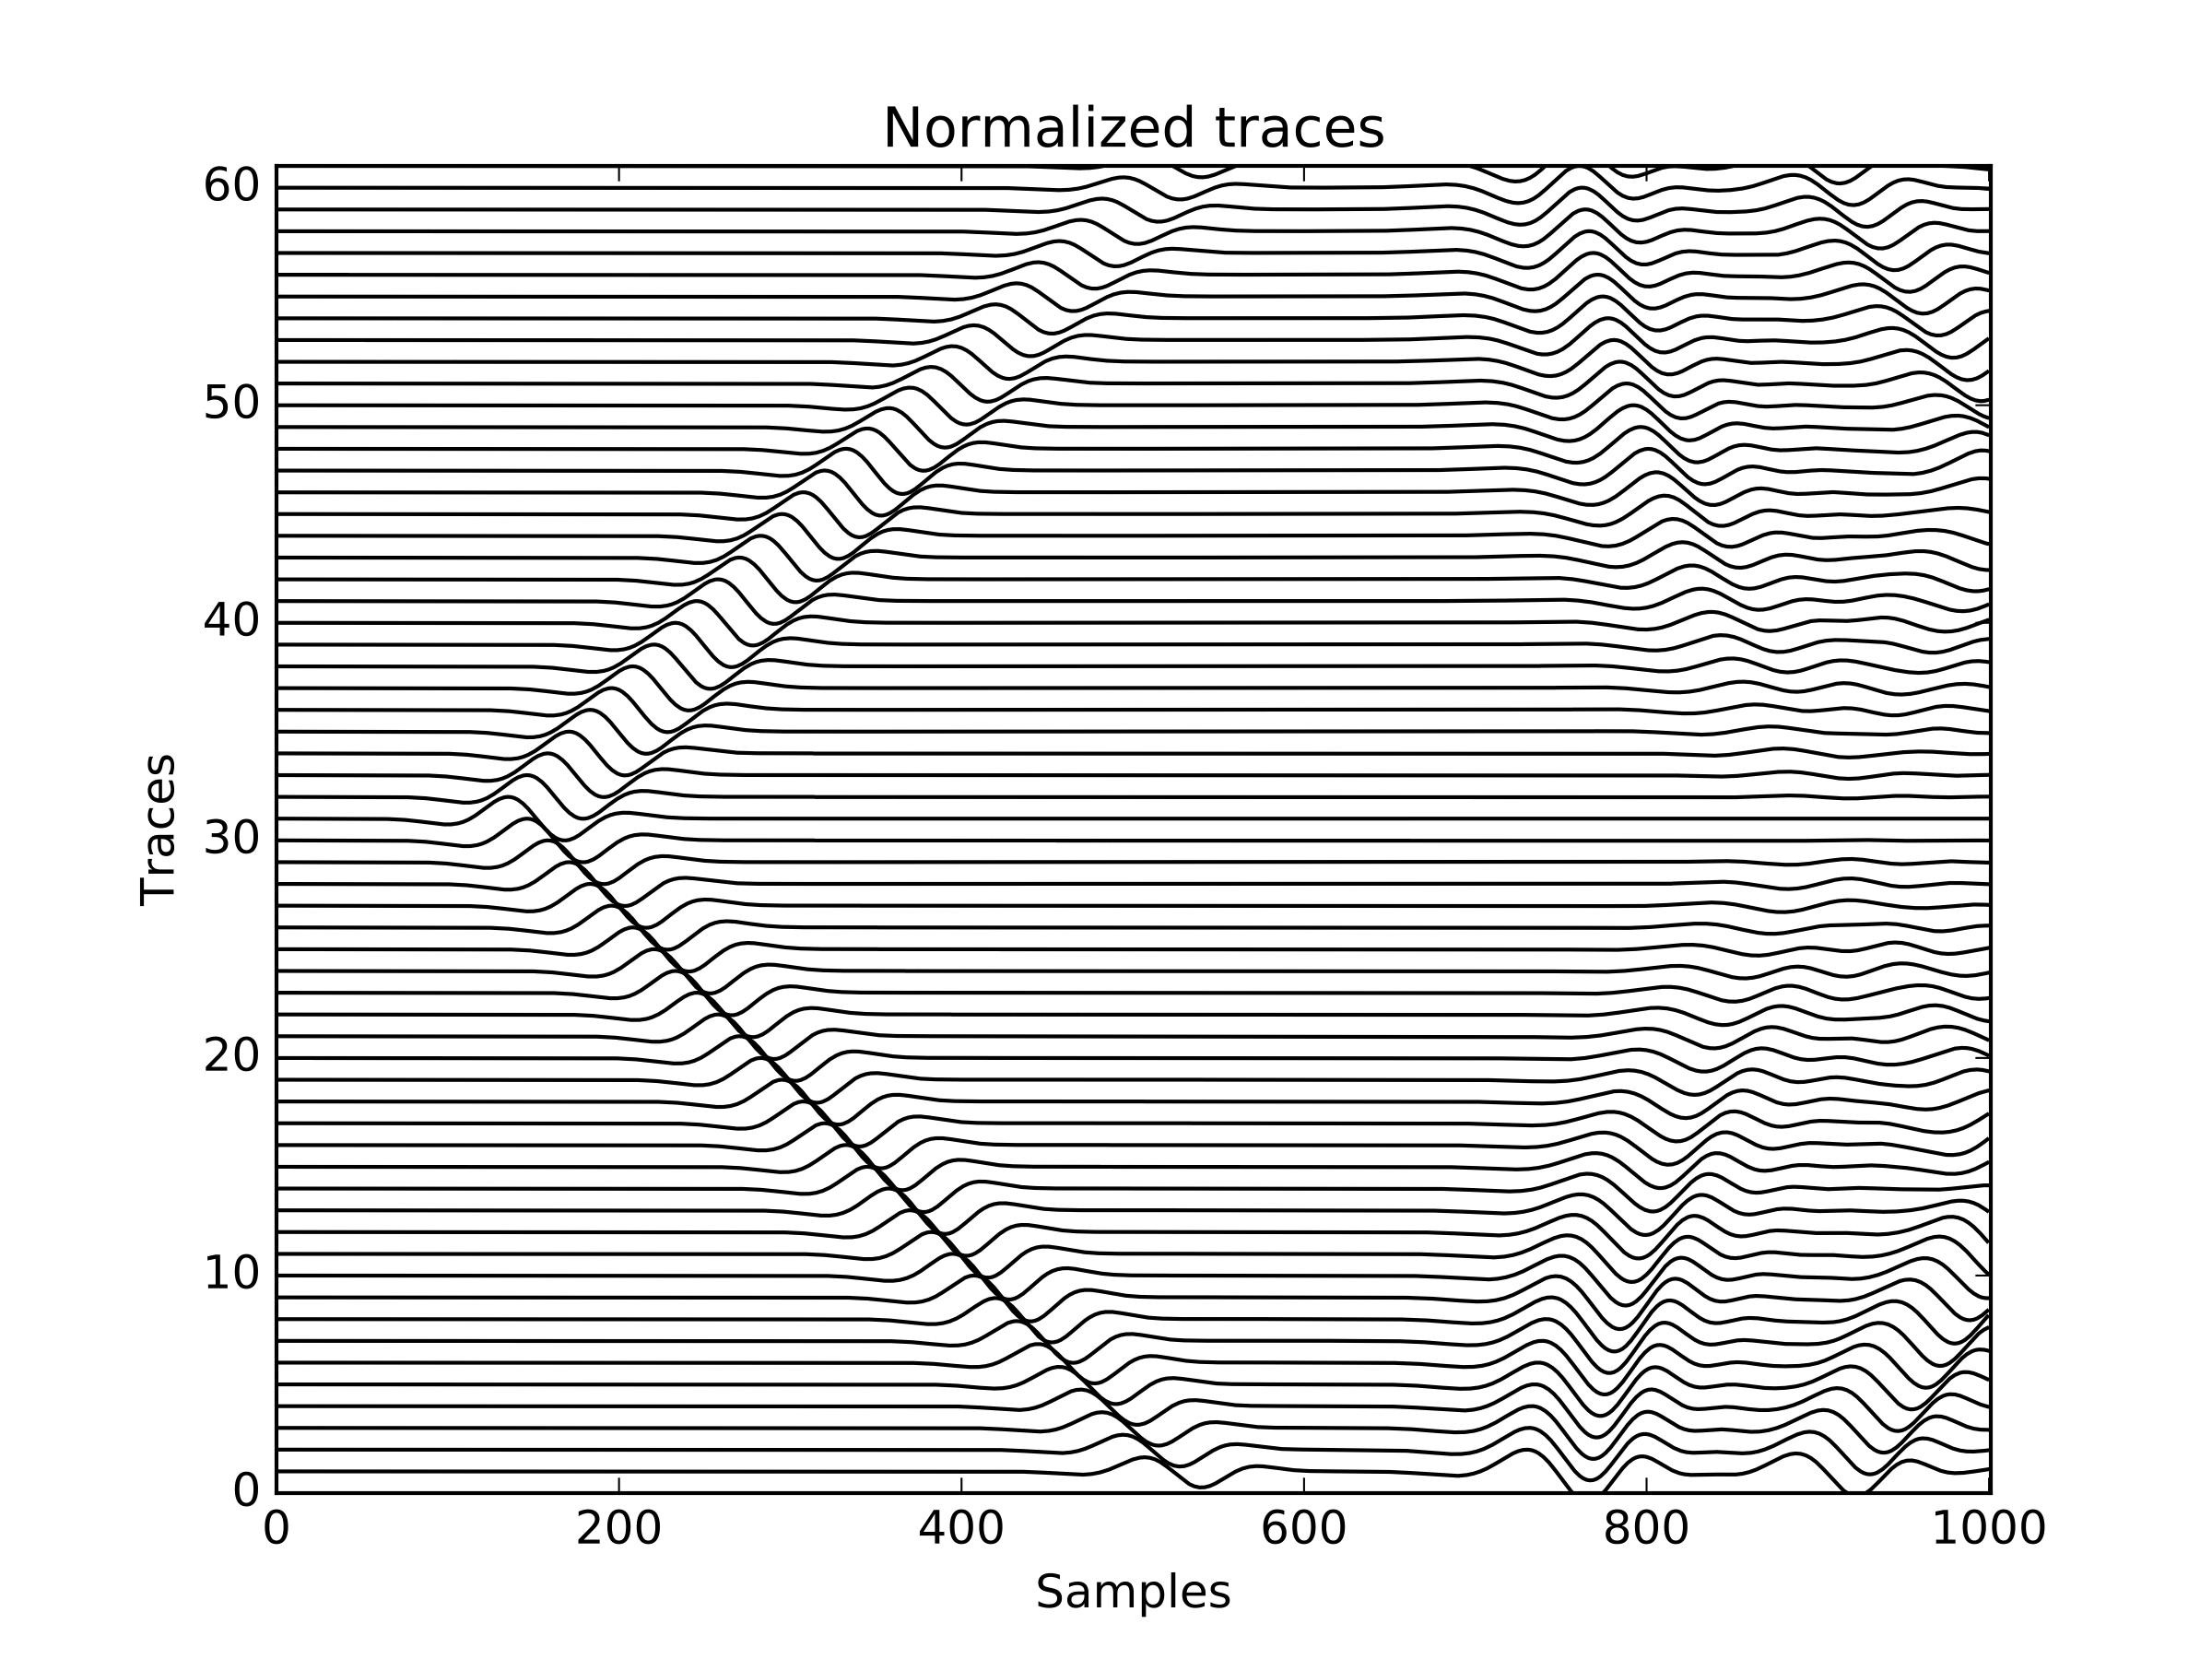
\includegraphics[width = .8\textwidth]{images/Test_Seismogram.png}
	\caption[Example pressure seismogram.]{Example pressure seismogram with 2nd order FD-operator and the default values: $NX=NY=NZ=100$, $v_p=\SI{3500}{m\per s}$ and $\rho = \SI{2000}{kg\per\cubic\metre}$.}\label{fig:Seismogram}
\end{figure}

\section{Configuration}\label{sec:config}
As mentioned in the quick guide, the configuration can be found in \shellcmd{par/configuration/}. In the \shellcmd{configuration.txt} file input variables can be added or changed. A list of all variables and config parameters that can be added and changed can be found in tables \ref{tab:config_grid} to \ref{tab:config_snapshots}.

\subsection{Configuration file}
\begin{table}[h!]
\caption[List of simulation/grid configuration parameters.]{List of simulation/grid configuration parameters, that can be added and changed in the config-file.}\label{tab:config_grid}
\centering
\begin{adjustbox}{width=1\textwidth,center=\textwidth}
	\begin{tabular}{llll}
	\toprule
	Variable & Short description & Type & Example value \\
	\midrule
	dimension & Dimension of the model (2D, 3D)  & string & 3D\\
	equationType & Type of the wave equations & string & acoustic \\
	NX & Number of grid points in $x$-direction & int & \num{100} \\
	NY & Number of grid points in $y$-direction & int & \num{100} \\
	NZ & Number of grid points in $z$-direction & int & \num{100} \\
	x0 & Starting position in $x$-direction & double & \num{0.0} \\
	y0 & Starting position in $y$-direction & double & \num{0.0} \\
	z0 & Starting position in $z$-direction & double & \num{0.0} \\
	DH & Distance between two grid points & double & \SI{50}{m}\\
	DT & Temporal sampling & double & \SI{2.0e-3}{s}\\
	T & Total simulation time & double & \SI{2}{s}\\
	spatialFDorder & Define order of spatial FD operator  & int & \num{2}\\
	\midrule
	useStreamConfig & Use a streaming configuration with model per shot & int & \num{0} \\
	streamConfigFilename & Filename of the stream configuration file & string & \begin{tabular}{@{}l@{}}\shellcmd{configuration/} \\\shellcmd{configurationStream.txt}\end{tabular} \\
	\midrule
	useVariableGrid & Use the variable Grid & int & \num{0} \\
	partitioning & Number of partitions & int & \num{1} \\
	useVariableFDoperators & Usage of variable FD operators & int & \num{0} \\
	graphPartitionTool & Partition Tool & string & geoKmeans\\
	gridConfigurationFilename & Filename to read grid configuration & string & \begin{tabular}{@{}l@{}}\shellcmd{configuration/} \\\shellcmd{gridConfigure.txt}\end{tabular} \\
	writePartition & Write partition to disk & int & \num{0} \\
	partitionFilename& Filename of the partition & string & \shellcmd{partition/partition}\\
	writeCoordinate & Write coordinates to disk & int & \num{0} \\
	coordinateFilename & Filename of the coordinates & string & \begin{tabular}{@{}l@{}}\shellcmd{configuration/} \\\shellcmd{coordinates}\end{tabular} \\
	ShotDomainDefinition & Define domains by ProcNS, node id or var \shellcmd{DOMAIN}  & int & \num{0} \\
	NumShotDomains & Define number of shot domains & int & \num{1} \\
	\bottomrule
	\end{tabular}
	\end{adjustbox}
\end{table}
\subsubsection{Simulation/grid}
The parameters can be divided in seven main groups. The first group which can be found in table \ref{tab:config_grid} contains the dimension (2D or 3D) and the type of wave equation (acoustic, sh, elastic, viscoelastic, tmem, emem, viscotmem, viscoemem), as well as parameters to describe the model (\verb+NX+, \verb+NY+, \verb+NZ+, \verb+x0+, \verb+y0+, \verb+z0+ and \verb+DH+) and temporal parameters (\verb+DT+ and \verb+T+). Please be careful in setting \verb+DH+ and \verb+DT+ to avoid the grid dispersion and the Courant instability. \verb+x0+, \verb+y0+ and \verb+z0+ are asked in the joint inversion. The total number of gridpoints is given by 
\begin{equation*}
	N=NX\times NY\times NZ
\end{equation*}
The total Number of time-steps can be calculated by 
\begin{equation*}
	NT = round\left(\frac{T}{DT}+0.5\right)
\end{equation*}
Furthermore, the parameter \verb+spatialFDorder+ defines the order of the spatial FD-operator and therefore influences the accuracy of the simulation significantly.

If the model is very large or a huge number of shots is used, it is useful to split the model into subsets. This can be done by setting the parameter \verb+useStreamConfig+ = 1. This allows for wavefield simulations within several model subsets that can be looped and cut at specific coordinates which would be automatically output to the file \verb+cutCoordinatesFilename+ as follows:
\begin{verbatim}
# Coordinate for cutting model per shot 
# ShotNumber | index_x | index_y | index_z
           0         0         0         0
           1        50         0         0
           2       100         0         0
\end{verbatim}
The number of rows, in this case three, specifies the number of unique shot used. The whole input model then is not specified by \verb+ModelFilename+ in the \shellcmd{configuration.txt} anymore, but by \verb+ModelFilename+ defined in the stream configuration file \verb+streamConfigFilename+. For each unique shot, we cut a model subset from the stream/big model defined in file \verb+streamConfigFilename+. The cutting coordinates are specified by the distance between the corresponding shot and the left most shot. The left or right distance between model boundaries and the unique shot in $x$-direction is identified with the left most or right most shot to avoid the artificial reflections caused by model cutting. Each model subset has the same model size $N$, which makes sure \verb+NumShotDomains+ shots can be generated parallelly with significantly lower computation cost than that directly running on a stream/big model. To sum up, \verb+NX+, \verb+NY+, \verb+NZ+, \verb+DH+, \verb+ModelFilename+, \verb+SourceFilename+ and \verb+ReceiverFilename+ in the file \verb+streamConfigFilename+ will be used to extract models per shot by setting \verb+useStreamConfig+ = 1. The other parameters in the \shellcmd{configuration.txt} file are then used for the model subset where the simulation is run. 

The following parameter \verb+useVariableGrid+ characterises whether the model uses a variable grid spacing for the calculation of the wavefield ($1=$ yes, else $=$ no). 
The type of partition can be chosen in \verb+partitioning+ where you can opt for a block distribution ($=0$), grid distribution ($=1$) parallel graph distribution by geographer ($=2$) or parallel graph distribution by ParMETIS ($=3$).
The block distribution divides the model vector evenly which creates a layered grid, the grid distribution divides the grid into equally large regions and the two graph distribution divides the grid based on optimal load balance and communication.
Variable FD operators can be used by \verb+useVariableFDoperators+ $=1$.

If a graph distribution is used (\verb+partitioning+ $=2$), you can choose in \verb+graphPartitionTool+ other partitioning tools (geographer, geoKmeans, geoHierKM, geoSFC, zoltanRIB, zoltanRCB, zoltanMJ, parMetisGeom or parMetisGraph).
The grid configuration can be read from a file and partitions and used coordinates can be written to disk if needed for plotting.

The last two parameters configure the shot domain parallelisation where two shot domains can be computed simultaneously. 
\verb+ShotDomainDefinition+ defines the domains by either ProcNS ($=0$), node id ($=1$) or an environment variable \shellcmd{DOMAIN} ($=2$).
If set to 0, the number of simultaneously computed shots is set by \verb+NumShotDomains+. If set to 1, the shot domains are set by nodes. Each node processes one domain. If set to 2, an environment variable called \shellcmd{DOMAIN} defines the domains.
Heterogenous clusters benefit if \verb+ShotDomainDefinition+ is set to 1 or 2. If set to 2, the load balance can be adjusted by another environment variable called \shellcmd{WEIGHT} (1.0 is default) which weights each domain. 
The weight of a domain is the sum of the weights of the corresponding processors for each domain. Depending on the weight, a domain is assigned to certain number of shots.
\shellcmd{DOMAIN} and \shellcmd{WEIGHT} can be set by a settings file where its name is set as an environment variable, e.g. by \shellcmd{export SCAISETTINGS=mySettings.txt}.
The file can look like this 
\begin{verbatim}
computer_name1 0-1 DOMAIN=0 WEIGHT=2
computer_name1 2-3 DOMAIN=1 WEIGHT=2
computer_name2 0 DOMAIN=2 WEIGHT=5 SCAI_CONTEXT=CUDA SCAI_DEVICE=0
computer_name2 1 DOMAIN=3 WEIGHT=5 SCAI_CONTEXT=CUDA SCAI_DEVICE=1
\end{verbatim}
where the first value represents the computer or node name, the second value the processors or node rank which can be set as an interval. In addition, GPUs can also be used if \shellcmd{SCAI\_CONTEXT} is set to CUDA.

\subsubsection{Input/output model}
\begin{table}[h!]
\caption[List of input/output model configuration parameters.]{List of input/output model configuration parameters, that can be added and changed in the config-file.}\label{tab:config_inputoutput}
\centering
\begin{adjustbox}{width=0.8\textwidth,center=\textwidth}
	\begin{tabular}{llll}
	\toprule
	Variable & Short description & Type & Example value \\
	\midrule	 
	ModelRead& Read model from File  & int & \num{0}\\
	ModelFilename& Filename-prefix to read model & string & \shellcmd{model/model}\\
	FileFormat&  File format of models and wavefields & int & \num{0}\\
	\bottomrule
	\end{tabular}
	\end{adjustbox}
\end{table}
\begin{table}[h!]
\caption[]{List of equationType and the corresponding model parameters.}\label{tab:equationType_model}
\centering
\begin{adjustbox}{width=0.8\textwidth,center=\textwidth}
	\begin{tabular}{ll}
	\toprule
	equationType & model parameter (suffix) \\
	\midrule	 
	acoustic & $v_p$ ("vp"), $\rho$ ("density")\\
	sh & $v_s$ ("vs"), $\rho$ ("density")\\
	elastic & $v_p$ ("vp"), $v_s$ ("vs"), $\rho$ ("density")\\
	viscoelastic & \begin{tabular}{@{}l@{}}{$v_p$ ("vp"), $v_s$ ("vs"), $\rho$ ("density"),} \\{$\tau^p$ ("tauP"), $\tau^s$ ("tauS")}\end{tabular} \\
	tmem and emem & $\sigma_e$ ("sigmaEM"), $\varepsilon_r$ ("epsilonEMr") \\
	viscotmem and viscoemem & \begin{tabular}{@{}l@{}}{$\sigma_e$ ("sigmaEM"), $\varepsilon_r$("epsilonEMr"),} \\{$\tau_{\sigma e r}$  ("tauSigmaEMr"), $\tau_{\varepsilon}$ ("tauEpsilonEM")}\end{tabular} \\
	\midrule
	* petrophysical parameter & $\phi$ ("porosity"), $S_w$ ("saturation")\\
	\end{tabular}
	\end{adjustbox}
\end{table}
The second section in table \ref{tab:config_inputoutput} contains parameters to manage input and output of the model. The first parameter \verb+ModelRead+ can be set with ($1=$ yes) or (else $=$ no). An on-the-fly model described in table \ref{tab:config_onthefly} will be created if there is no input model. \verb+ModelFilename+ is given to determine the location and filename of the model. \verb+ModelFilename+ is only a prefix to read the model data in directory \shellcmd{model/}. The filename ending is added automatically depending on which model is needed (e.g. \shellcmd{model.suffix.mtx}) while the file format is configured in \verb+FileFormat+ with either $1=$ mtx, a formated ascii file with serial input/output, $2=$ lmf, a binary file with parallel input/output, little endian and a 5 int header (20 byte) or $3=$ frv, a binary file with serial input/output,  little endian and seperate header. Due to the parallel input/output, choosing lmf as the file format is recommended. For different type of wave equation, the model parameters input (\verb+ModelRead+=1) or output (\verb+ModelRead+=0) are different. Please see details of the corresponding suffix added to ModelFilename in table \ref{tab:equationType_model}. The model files of porosity $\phi$ (\verb+suffix+ = ``porosity'') and saturation $S_w$ (\verb+suffix+ = ``saturation'') are not necessary for WAVE-Simulation, but they are needed in petrophysical inversion in WAVE-Inversion.

\subsubsection{On-the-fly seismic model}
\begin{table}[h!]
\caption[List of on-the-fly seismic model configuration parameters.]{List of on-the-fly seismic model configuration parameters, that can be added and changed in the config-file.}\label{tab:config_onthefly}
\centering
\begin{adjustbox}{width=0.8\textwidth,center=\textwidth}
	\begin{tabular}{llll}
	\toprule
	Variable & Short description & Type & Example value \\
	\midrule
	velocityP & P-wave velocity $v_p$ in meter per seconds & double & \SI{3500}{m\per s} \\
	velocityS& S-wave velocity $v_s$ in meter per seconds & double  & \SI{2000}{m\per s}\\
	rho& Density $\rho$ in kilogram per cubic meter & double &  \SI{2000}{kg\per\cubic\metre}\\
	tauP& $\tau$ value for P-waves & double & \num{0.0}\\
	tauS& $\tau$ value for S-waves & double & \num{0.0}\\
	\bottomrule
	\end{tabular}
	\end{adjustbox}
\end{table}
In the third section in \ref{tab:config_onthefly} all variables can be set to create a homogeneous seismic model on-the-fly. The variable \verb+velocityP+ ($v_p$) is only needed in elastic and viscoelastic calculations and  \verb+tauP+ ($\tau^p$) and \verb+tauS+ ($\tau^s$) are solely needed in the viscoelastic case. 
The P-wave ($\pi$) and S-wave ($\mu$) moduli can be calculated by:
\begin{align*}
	\pi&=\rho\cdot v_p^2\\
	\mu &=\rho\cdot v_s^2\\
\end{align*}
The Matlab script \shellcmd{createHomogeneousModel.m} and the Python script \shellcmd{createHomoge- neousModel.py} in \shellcmd{model/} are examples how to generate external models in both mentioned parametrisation. 
To verify the models stability  the courant can be calculated: 
\begin{equation*}
	v_{max} \cdot \frac{DT}{DH} \leq 0.43
\end{equation*}

\subsubsection{Viscoelastic and visco-EM wave modelling}
\begin{table}[h!]
\caption[List of viscoelastic and visco-EM wave modelling configuration parameters.]{List of viscoelastic and visco-EM wave modelling configuration parameters, that can be added and changed in the config-file.}\label{tab:config_visco}
\centering
\begin{adjustbox}{width=1\textwidth,center=\textwidth}
	\begin{tabular}{llll}
	\toprule
	Variable & Short description & Type & Example value \\
	\midrule
	numRelaxationMechanisms & Number of relaxation mechanisms & int & \num{0}\\
	relaxationFrequency& Relaxation frequency& double & \SI{0}{Hz}\\
	\bottomrule
	\end{tabular}
	\end{adjustbox}
\end{table}
The fourth section in \ref{tab:config_visco} are the parameters relevant for viscoelastic and visco-EM wave modelling. The two parameters of this table-section describe the number of relaxation mechanisms and the relaxation frequency for first relaxation mechanism (given in \SI{}{Hz}).

\subsubsection{Boundary conditions}
\begin{table}[h!]
\caption[List of boundary conditions configuration parameters.]{List of boundary conditions configuration parameters, that can be added and changed in the config-file.}\label{tab:config_boundary}
\centering
\begin{adjustbox}{width=1\textwidth,center=\textwidth}
	\begin{tabular}{llll}
	\toprule
	Variable & Short description & Type & Example value \\
	\midrule
	FreeSurface& Use the free surface (0, 1, 2) & int & \num{0}\\
	DampingBoundary& Use the damping Boundary (0, 1, 2) & int & \num{0}\\
	BoundaryWidth& Width of damping boundary & int & \num{10}\\
	DampingCoeff& Damping coefficient & double & \num{8.0}\\
	VMaxCPML& Maximum velocity of the CPML & double &\SI{3500}{m\per s}\\
	CenterFrequencyCPML\;\;\;\;& Center frequency inside the boundaries\;\;\;  & double &\SI{5}{Hz}\\
	NPower& Degree of the damping profile & int &\num{4}\\
	\bottomrule
	\end{tabular}
	\end{adjustbox}
\end{table}
The fifth part in table \ref{tab:config_boundary} handles the boundary conditions. In EM wave simulation, the free surface can be turned off by setting (\verb+FreeSurface+ $=0$). In this case the model boundary is also used at the top. If you want to use a free surface in seismic wave simulation two methods are implemented. By selecting (\verb+FreeSurface+ $=1$) the mirror method is chosen. This method only works for a flat surface which is represented by the upper edge of the model. Selecting (\verb+FreeSurface+ $=2$) chooses the Improved Vacuum Formulation (IVF). This method should be chosen in case of a free surface with topography but requires additional grid points above the highest surface elevation. The number of additional grid points must be at least equal to one plus half the length of the FD operator if the medium above the free surface is vacuum. IVF is used regardless of your choise of \verb+FreeSurface+ but it only affects you if there is a medium with density or in elastic case shear modulus of zero in the model. Without this behaviour the simulation would crash in this case. The only difference between (\verb+FreeSurface+ $=0$) and (\verb+FreeSurface+ $=2$) is that the absorbing boundary at the top is turned off in the later case. So if you choose to discretize air at the top of your model you need to select (\verb+FreeSurface+ $=0$) and introduce additional grid points equal to the thickness of your boundary. 
The model boundaries are characterised by \verb+DampingBoundary+, \verb+BoundaryWidth+ and \verb+DampingCoeff+. 
The usage of damping boundaries can be turned off (\verb+DampingBoundary+ $=0$) or set as ABS $=1$ or CPML $=2$. Again, if the parameter for \verb+DampingBoundary+ is set to 0, it is not used. 
If \verb+CPML+ is used, \verb+VMaxCPML+, \verb+CenterFrequencyCPML+ and \verb+NPower+ also have to be set. 

\subsubsection{Acquisition geometry}
\begin{table}[h!]
\caption[List of acquisition geometry configuration parameters.]{List of acquisition geometry configuration parameters, that can be added and changed in the config-file.}\label{tab:config_acquisition}
\centering
\begin{adjustbox}{width=1\textwidth,center=\textwidth}
	\begin{tabular}{llll}
	\toprule
	Variable & Short description & Type & Example value \\
	\midrule
	SourceFilename & Filename-prefix to read source configuration & string & \begin{tabular}{@{}l@{}}\shellcmd{acquisition/} \\\shellcmd{sources}\end{tabular}  \\
	ReceiverFilename & Filename-prefix to read receiver configuration & string & \begin{tabular}{@{}l@{}}\shellcmd{acquisition/} \\\shellcmd{reciever}\end{tabular}  \\
	SourceSignalFilename & Filename-prefix to read source signal & string & \begin{tabular}{@{}l@{}}\shellcmd{acquisition/} \\\shellcmd{signal}\end{tabular}  \\
	useReceiversPerShot & Use different receivers for each shot (0, 1, 2) & int & \num{0} \\
	useRandomSource & Use random sources (0, 1, 2) & int & \num{0} \\
	RandomSourceFilename & Filename to record random source numbers & string & \begin{tabular}{@{}l@{}}\shellcmd{acquisition/} \\\shellcmd{randomSources.txt}\end{tabular}  \\
	writeSource & Write used source wavelet per shot & int & \num{0}\\	
	WriteSourceFilename & Filename-prefix to write source wavelet & string & \begin{tabular}{@{}l@{}}\shellcmd{SourceSignal/} \\\shellcmd{Source}\end{tabular}  \\
	SeismogramFilename & Filename-prefix to write seismograms & string & \begin{tabular}{@{}l@{}}\shellcmd{seismograms/} \\\shellcmd{seismogram}\end{tabular}  \\
	seismoDT & Seismogram sampling in seconds & double & \num{0.002} \\
	normalizeTraces & Normalize the seismogram-traces & int & \num{0}\\
	envelopTraces & Envelop the seismogram-traces & int & \num{0}\\
	SeismogramFormat & Seismogram format & int & \num{1}\\
	initSourcesFromSU & Initialize sources from SU file & int & \num{0}\\
	initReceiverFromSU & Initialize receivers from SU file & int & \num{0}\\
	\bottomrule
\end{tabular}
\end{adjustbox}
\end{table}
The sixth section in \ref{tab:config_acquisition} handles the acquisition geometry. \verb+SourceFilename+ and \verb+ReceiverFilename+ must be set to the files where source and receiver properties are specified respectively. The ending .txt has to be omitted in the config-file. 
\verb+SourceSignalFilename+ specifies the location of the file where the source signals are stored in case you want to use your own.
\verb+useReceiversPerShot+ = 0 means all shot have the same receiver configuration. If \verb+useReceiversPerShot+ = 1, you can use an individual receiver configuration for each shot. In this case you need as many receiver files as there are shots. Therefore all receiver files must have the ending \shellcmd{.shot\_<shot number>.txt}. 
Alternatively, \verb+useReceiversPerShot+ = 2 can be used to save much storage memory compared with \verb+useReceiversPerShot+ = 1.
By setting \verb+useReceiversPerShot+ = 2, you have to define all receivers position and receiver type in \verb+ReceiverFilename+ and define an additional file \verb+ReceiverFilename.mark.mtx+ to identify which receivers are used for each shot. Please see \ref{sec:sourcesandreceiver} for more details of how  \verb+SourceFilename+, \verb+ReceiverFilename+ and \verb+ReceiverFilename.mark.mtx+ are structured.  \verb+useRandomSource+ has to be set 0 in forward modelling so that all shots are simulated. In inversion, however, one can set \verb+useRandomSource+ = 1 to randomly choose or set \verb+useRandomSource+ = 2 to sequentially choose \verb+NumShotDomains+ shots at each iteration, which will significantly speed up the inversion progress. The file \verb+RandomSourceFilename+ is used to output the source numbers selected in random shot inversion \verb+useRandomSource+ = 1 or sequential shot inversion \verb+useRandomSource+ = 2.
The used source wavelet per shot can be written to disk by setting \verb+writeSource+ to 1 and specifying a filename \verb+WriteSourceFilename+.
\verb+SeismogramFilename+ gives the location where the modelled seismograms are stored. Their sampling can be set in seconds in \verb+seismoDT+ and their traces can be normalized by setting \verb+normalizeTraces+ to 1 or be enveloped by setting \verb+envelopTraces+ to 1. Note that \verb+seismoDT+ must be the same as or smaller than \verb+DT+ in inversion because the seismograms obtained in forward modelling are used to generate an adjoint source for back propagation of wavefields. That means if we set \verb+seismoDT+ > \verb+DT+, the Courant instability will occur in the back propagation.
These seismograms can be saved in mtx $=1$, lmf $=2$, frv $=3$ or SU $=4$ format depending on the value of \verb+SeismogramFormat+.  
Furthermore, the sources or receivers can be initialized from SU files if \verb+initSourcesFromSU+ and \verb+initReceiverFromSU+ is set to 1.

\subsubsection{Wavefield snapshots}
\begin{table}[h!]
\caption[List of wavefield snapshots configuration parameters.]{List of wavefield snapshots configuration parameters, that can be added and changed in the config-file.}\label{tab:config_snapshots}
\centering
\begin{adjustbox}{width=1\textwidth,center=\textwidth}
	\begin{tabular}{llll}
	\toprule
	Variable & Short description & Type & Example value \\
	\midrule
	snapType & Type of wavefield snapshots to save & int & \num{1} \\
	WavefieldFilename & Name and location where to save snapshots & string & \begin{tabular}{@{}l@{}}\shellcmd{wavefields/} \\\shellcmd{wavefield}\end{tabular}  \\
	tFirstSnapshot & Time of first snapshot in seconds & double & \num{0.1} \\
	tLastSnapshot & Time of last snapshot in seconds & double & \num{2.2} \\
	tIncSnapshot & Time interval between snapshots  in seconds & double & \num{0.1} \\
	\midrule
    verbose        & display detailed output                          &  int   & 0 \\
	
	\bottomrule
	\end{tabular}
	\end{adjustbox}
\end{table}	
In the last section in \ref{tab:config_snapshots} you can set the properties of the wavefield snapshots to save. \verb+snapType+ sets the wavefield type that should be saved ($0=$ no save, $1=$ save velocities, $2=$ save pressure/stress, $3=$ save energy). 
The snapshots are stored in the directory chosen in \verb+WavefieldFilename+. Snapshots start at time \verb+tFirstSnapshot+, end at time \verb+tLastSnapshot+ and have an interval of \verb+tIncSnapshot+.

At the end of configuration file, one can set \verb+verbose+ = 0 to briefly display the key points of the program running, or \verb+verbose+ = 1 to show all the status messages which can be confusing if shots are run in parallel. However, \verb+verbose+ = 1 would help you find the bugs much faster when you develop and debug a new feature in WAVE-Simulation.

\subsection{Source and Receiver File}\label{sec:sourcesandreceiver}
In \shellcmd{par/acquisition/} two files can be found,the \shellcmd{sources.txt} and \shellcmd{receiver.txt} files.
The source file contains columns filled with information about the source number, source coordinates (x, y, z), source type, wavelet shape, center frequency, amplitude and time shift. It can look like this
\begin{verbatim}
# shotNr x  y  z  sourceType WAVELET_TYPE WAVELET_SHAPE FC AMP TShift
  0      50 50 50 3          1            1             5  5   0
  1      40 40 40 1          1            1             5  5   0
  1      80 80 80 1          1            1             5  5   0
\end{verbatim}
where each row is one shot. Each shot with the same shot number is modelled in one simulation, whereas each shot number is simulated individually. Thus, the example shows two shot simulations, one with one shot, the other with two.
The coordinates in (x, y, z) are given in grid points. There are three different source types, pressure (1 = P or eZ), velocity in x- (2 = vX or eX), y- (3 = vY or eY), and z-direction (4 = vZ or hZ). 
The wavelet type can be set as 1 = synthetic signal or 0 = own signal and its shape can be set as a 1 = Ricker wavelet, 2 = Fuchs-M\"uller signal, 3 = $\sin^3$ function, 4 = First derivative of Gaussian, 5 = Spike/Delta signal, 6 = integral of $\sin^3$, and 7 = Ricker wavelet used in GprMax which is a GPR simulation software  \citep{giannopoulos2005modelling}. 
Further information can be found in chapter \ref{sec:sourcesignal}.
Center frequency is to be set in Hz, the Amplitude scales the maximum amplitude of the wavefields and output seismograms and the time shift is defined in seconds.

The receiver file is similarly built, with information about the receiver coordinates and the receiver type. It can look like this 
\begin{verbatim}
# x  y  z  receiver_type
  20 20 20 1
  21 21 21 1
  20 20 20 2
  21 21 21 2
\end{verbatim}
where each row is one receiver with its grid coordinates in (x, y, z) and receiver type that can be set as pressure (1 = P or eZ), velocity in x- (2 = vX or eX), y- (3 = vY or eY), and z-direction (4 = vZ or hZ). Depending on the chosen type, the output seismograms will have the same type. In case of \verb+useReceiversPerShot+ = 2, you have to define a file named \verb+ReceiverFilename.mark.mtx+ to store marks. The mark matrix maybe look like this
\begin{verbatim}
# shotNr receiver_mark (1=use, 0=not use)
  0      0 0 0 0 1 1 1 1 1 1 1 1 1 1 ...
  1      1 1 0 0 0 0 1 1 1 1 1 1 1 1 ...
  2      1 1 1 1 0 0 0 0 1 1 1 1 1 1 ...
\end{verbatim}
Please note you have to reshape this mark matrix to a vector and save it as mtx format.

\subsection{Source Signal}\label{sec:sourcesignal}
There are two ways to choose a source signal used for modelling the wavefield. First a synthetic source signal can be used to calculate the wave fields. The Software contains different source signals which can be chosen from. A visualisation of the signals is show in figure \ref{fig:Signal}. The built in wavelets are a signal given by the first derivative of the Gaussian, $\int sin^3$ wavelet, Ricker wavelet, $sin^3$ wavelet, Fuchs-M\"uller signal, a spike signal, and Ricker wavelet of GprMax (The last wavelet type are not ploted in this manual but you can find it from GprMax user manual \url{http://docs.gprmax.com/en/latest/}). The corresponding equations are given by equation \ref{eqn:SignalStart} to \ref{eqn:SignalEnd}, where $A$ is the wavelet amplitude.
\begin{figure}[h!]
\centering
	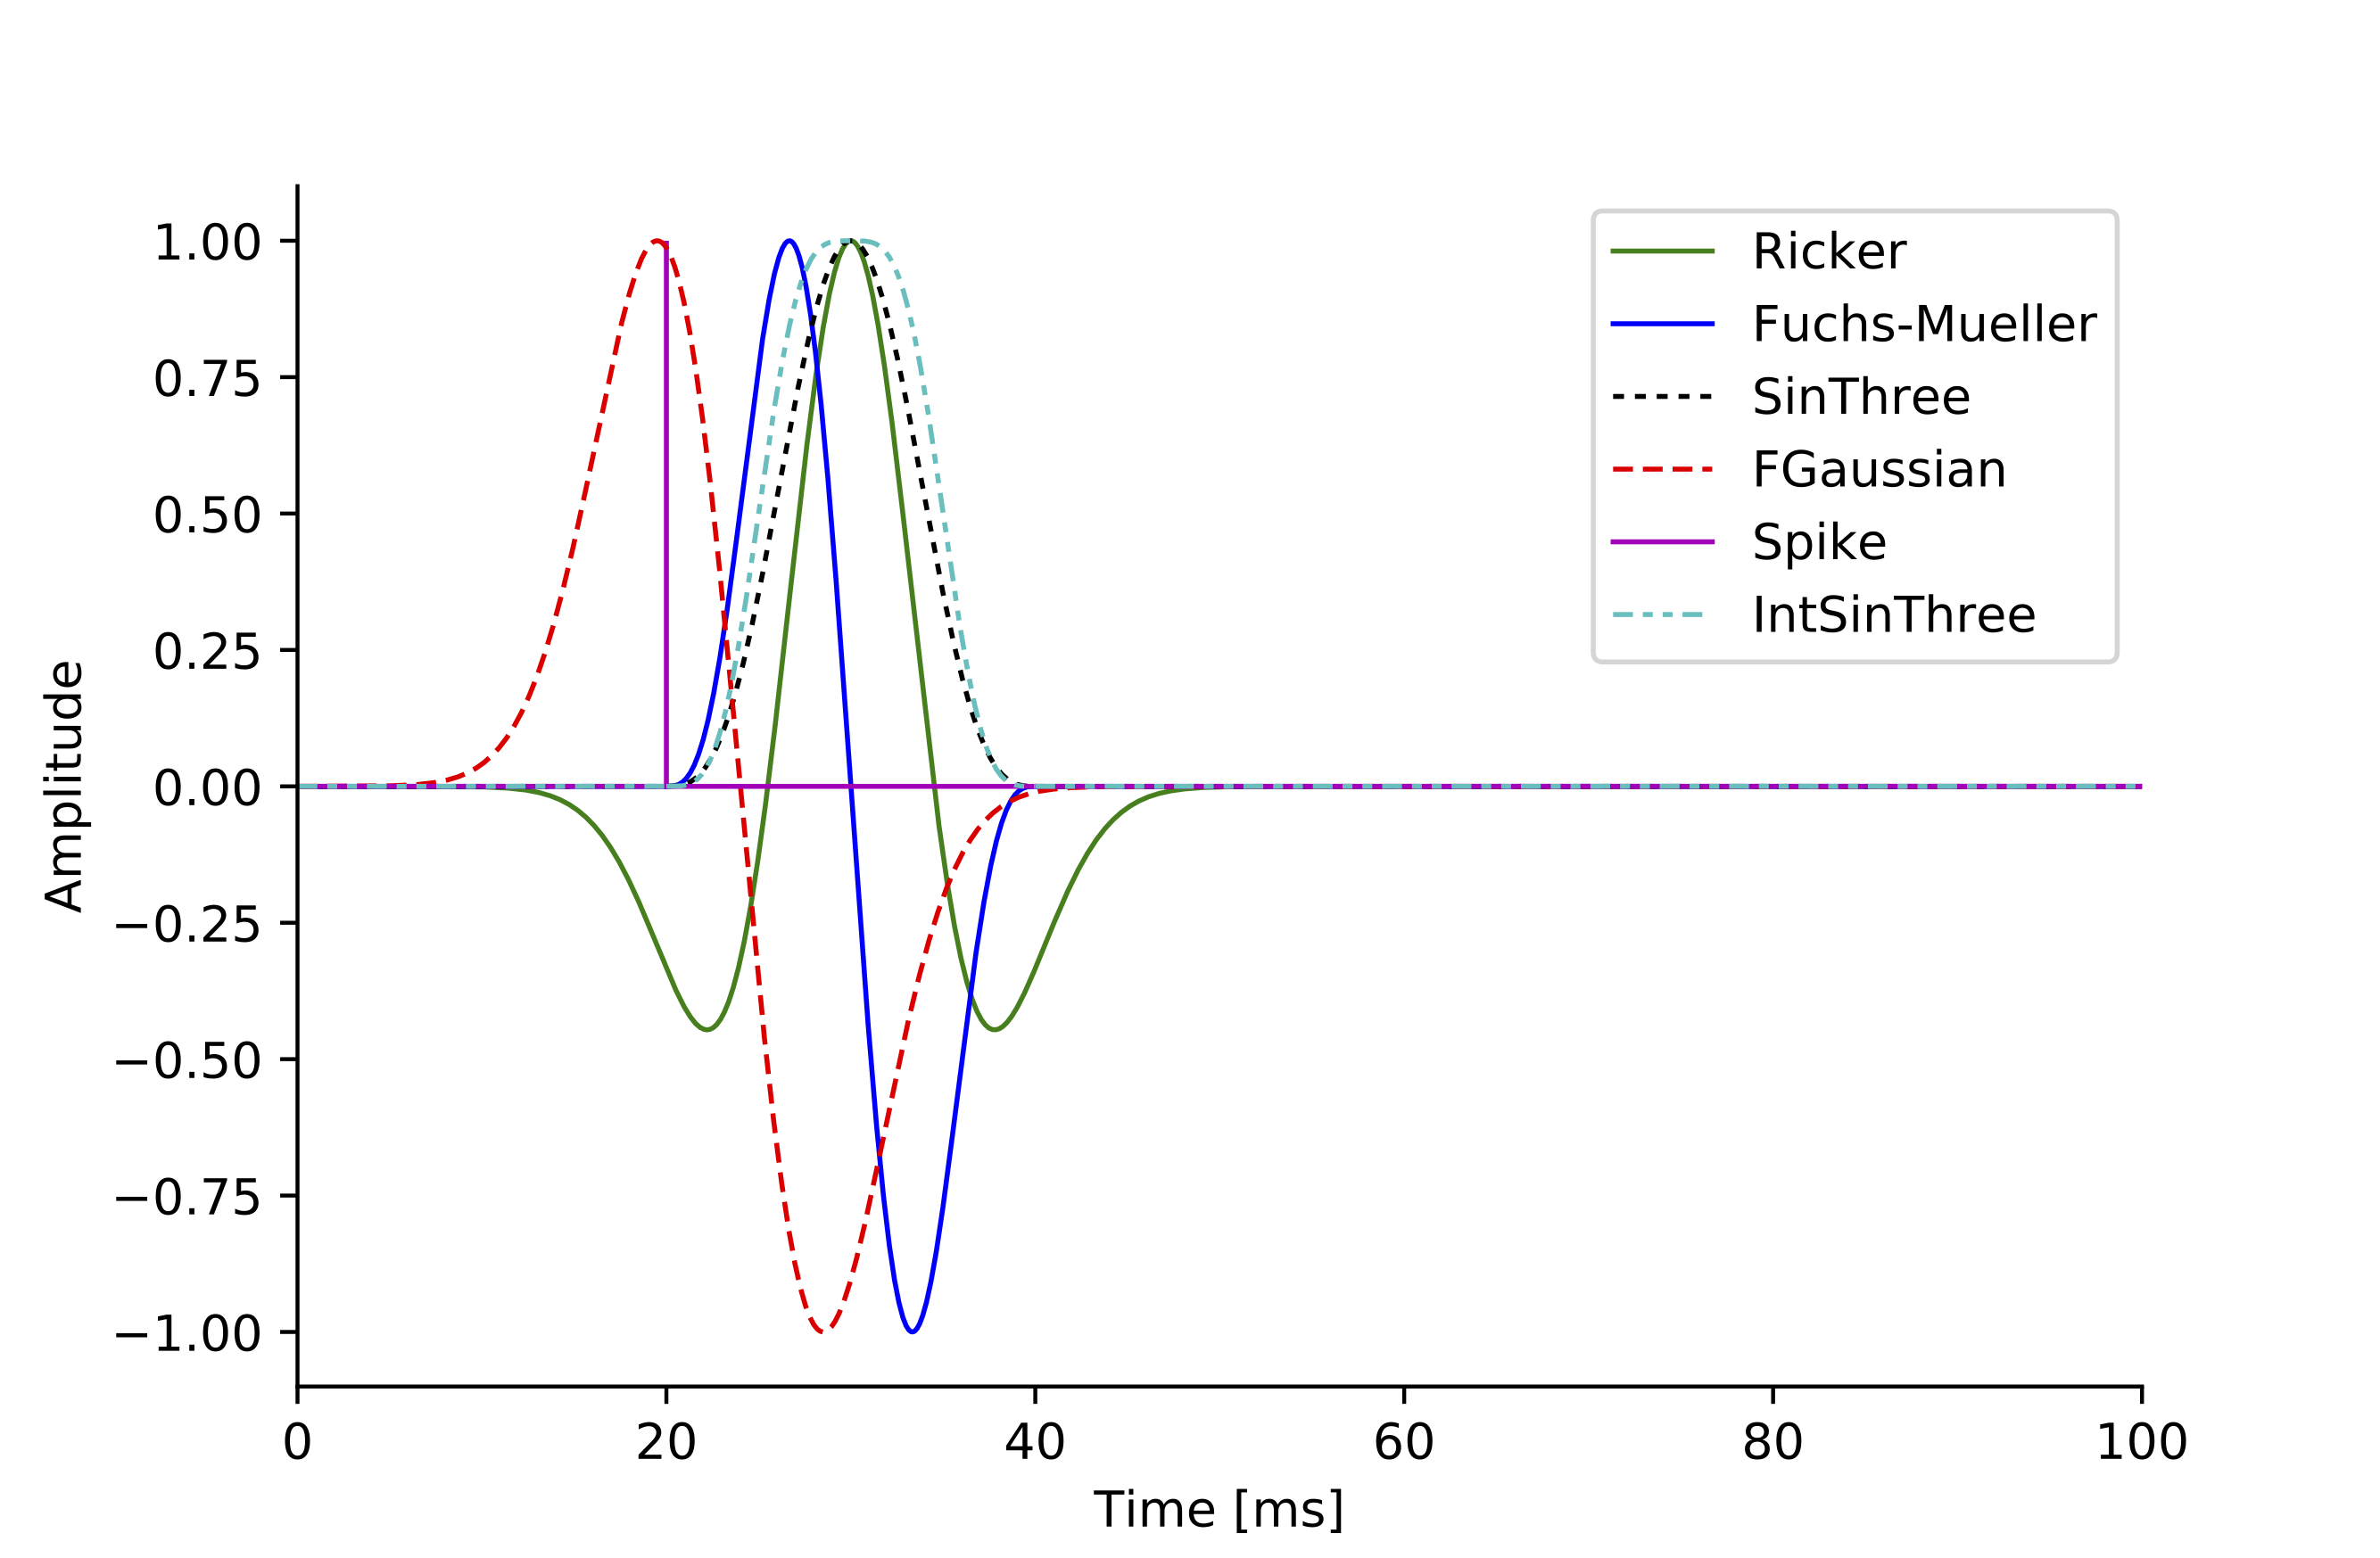
\includegraphics[width=.7\textwidth]{images/Signal_Plot.png}
	\caption[Plot of the different source wavelets.]{Plot of the different source wavelets (equation \ref{eqn:SignalStart} to \ref{eqn:SignalEnd}). All signals have an amplitude of $1$, a center frequency of $f_c = $\SI{50}{Hz} and a time-shift of $T_s=\nicefrac{1}{f_c}=$\SI{50}{ms}}\label{fig:Signal}
\end{figure}

\begin{itemize}
\item Ricker wavelet:
\begin{align}
	f(t) &= A \cdot \left(1 - 2\cdot\tau^2\right)\cdot e^{-\tau^2} \qquad \text{with} \qquad \tau=\pi\cdot f_c\cdot\left(t - \frac{1.5}{f_c}-T_s\right) \label{eqn:SignalStart}\\
\intertext{\item Fuchs-M\"uller signal, which is a combination of different sinus signals:}
	f(t)&= 
	\begin{cases}
		 \quad A\cdot\left(sin(\tau) - \frac{1}{2}sin(2\cdot\tau)\right)  & \qquad \text{if } \quad T_s\leq t\leq\left(T_s+\frac{1}{f_c}\right)\\
	\quad 0 & \qquad \text{otherwise}
	\end{cases}\\
	&\text{with} \qquad \tau=2\cdot \pi\cdot f_c\cdot\left(t -T_s\right)
\intertext{\item $sin^3$ signal:}
	f(t)&= 
	\begin{cases}
		 \quad A\cdot sin^3(\tau)  & \qquad \text{if } \quad T_s\leq t\leq\left(T_s+\frac{1}{f_c}\right)\\
	\quad 0 & \qquad \text{otherwise}
	\end{cases}\\
	&\text{with} \qquad \tau=\pi\cdot f_c\cdot\left(t -T_s\right)
\intertext{\item Signal given by the first derivative of the Gaussian:}
	f(t) &=-A \cdot 2 \cdot \tau \cdot e^{-\tau^2} \qquad \text{with} \qquad \tau=\pi\cdot f_c\cdot\left(t - \frac{1.2}{f_c}-T_s\right)\\
\intertext{\item Spike signal:}
	f(t)&= 
	\begin{cases}
		 \quad 1  & \qquad \text{if } \quad t = T_s \\
	\quad 0 & \qquad \text{otherwise}
	\end{cases}
\intertext{\item Wavelet given by the integral of $sin^3$: with $ \tau=\pi\cdot f_c\cdot\left(t - T_s\right)$}
	f(t)&= \label{eqn:SignalEnd}
	\begin{cases}
		 \quad \dfrac{A \cdot \left(\frac{1}{2} - \frac{3}{4}\cdot cos(\tau) + \frac{1}{4} \cdot cos^3(\tau)\right)}
	{f_c\cdot \pi \frac{3}{4}}  & \qquad \text{if } \quad T_s\leq t\leq\left(T_s+\frac{1}{f_c}\right)\\
	\quad 0 & \qquad \text{otherwise}
	\end{cases}
\intertext{\item Ricker wavelet of GprMax:}
	f(t) &=-A \cdot 2 \cdot \zeta \cdot \sqrt{e^{1/2\zeta}} \cdot e^{-\zeta \tau^2} \cdot \tau \quad \text{with} \quad \tau=\pi\cdot f_c\cdot\left(t - \frac{1.0}{f_c}-T_s\right), \zeta = 2 \pi^2 f^2
\end{align}
\end{itemize}
To create different source signals the \shellcmd{source.mtx} file can be generated with either the \shellcmd{createSource.m} or the \shellcmd{createSource.py} script. The scripts give the options to change the source type, the wavelet type, the wavelet shape ($1=$ Ricker, $2=$ Fuchs-M\"uller, $3=sin^3$, $4=$ FGaussian, $5=$ Spike, $6=$ Integral of $sin^3$, and $7=$ Ricker wavelet of GprMax), the center frequency in Hz, the Amplitude and the timeshift in s.  \\
The second way of setting a source function is using your own signal. There are two possibilities to do so. The first is using the same source signal for all shots and the second is using an individual signal for each shot. In both cases the source signal is read from the lines in the file set by \verb+SourceSignalFilename+. If you set the wavelet type to 2 only the first line of the source signal file is used as wavelet for all shots. If it's set to 3 the lines in this files are used successively for each shot. It's also possible to combine wavelet type 1 and 2 or 1 and 3. Only the combination 2 and 3 is prohibited. If you use your own source signal you have to take care that it has the same length and sampling as your simulation time. Also the file must have as many lines as you have sources with wavelet type 3. 

\clearpage
\section{Pre- and Post-Processing}\label{sec:process}

As already mentioned in section \ref{sec:config}, data can be read from a single file as well as from a partitioned file-block. The advantage of a distributed file system ist, that CPUs/GPUs can read data simultaneously and therefore with substantial timesaving. Installing LAMA with all examples (\shellcmd{-DBUILD\_EXAMPLES=ON}), LAMA includes examples to partition and repartition files or file-blocks in \shellcmd{.mtx}-format (\shellcmd{vectorRepartition.exe}). 

To partition a single vector-file change to the directory where the files are located and run the following comand:  \\
\shellcmdline{\$SCAI\_ROOT/lama/examples/io/vectorRepartition.exe filename.mtx 1 }\\
\shellcmdline{filename\_\%r.mtx <NProcessors>}\\
The first part marks the LAMA-example to repartition a file, \shellcmd{filename.mtx} is a single file (\shellcmd{1}) you want to partition and \shellcmd{filename\_\%r.mtx} is the name of the output file-block. The number of files in a file-block has to be the same as the number of CPUs/GPUs (\shellcmd{<NProcessors>}) reading the file-block later on. 

To merge a fileblock \shellcmd{filename\_\%r.mtx} to a single vector-file, the command is very similar:\\
\shellcmdline{\$SCAI\_ROOT/lama/examples/io/vectorRepartition.exe filename\_\%r.mtx}\\
\shellcmdline{<NProcessors> filename.mtx 1}\\
In this case the name of the file-block and its size is written fist and then the name of the single output-file.

\section{Unit Tests}
To guarantee a functioning framework, WAVE-Simulation includes unit-tests using the googletest framework. To run all unit-tests, you first have to install googletest (e.g. from \url{http://code.google.com/p/googletest}). 

As preparatory steps environment variables have to be linked to googletest. Add the following lines to the \shellcmd{{\char`\~}/.bashrc}:
\\\shellcmdline{ `export GTEST\_DIR=[PATH\_TO\_GTEST\_DIRECTORY]`}
\\\shellcmdline{ `export LD\_LIBRARY\_PATH=\$\{GTEST\_DIR\}:\$\{LD\_LIBRARY\_PATH\}`}
\\\shellcmdline{ `export DYLD\_LIBRARY\_PATH=\$\{GTEST\_DIR\}:\$\{DYLD\_LIBRARY\_PATH\}}

To compile all tests, change the directory: \\\shellcmdline{WAVE-Simulation/build/} \\ and compile the tests by simply entering:\\\shellcmdline{make utest} and \shellcmdline{make itest}

The executable file is located in the directory:
\\\shellcmdline{WAVE-Simulation/build/bin}\\
To execute the unit-tests change to the \shellcmd{/par} folder and run the \shellcmd{Test\_unit} file by entering:
\\\shellcmdline{./../build/bin/Test\_unit}\\ 
For faultless function of WAVE-Simulation all tests should execute without failure.

\section{Benchmark}

\subsection{Free surface}

As mentioned in \ref{sec:FreeSurface} there are two implementations of the free surface in WAVE-Simulation. To ensure their proper functionality they are tested against an analytic solution. This solution is for a homogeneous halfspace with a free surface. Tests are done in 2D for the acoustic and the elastic case. Relevant parameters used are listed in table \ref{tab:freeSurfaceBenchmark}. In the acoustic case the shear wave velocity for the analytic solution is set to 1 $m/s$ for a stable result. The results are shown in figure \ref{fig:IVFvsAnalytic} for IVF and in figure \ref{fig:MirrorvsAnalytic} for mirror method. Since there are no surface waves in the acoustic case only the P-phase is visible. The combination of high amplitude surface waves and trace normalization make the P-phase almost disappear in the elastic case. Both results show, that the methods used are able to produce accurate solutions even at larger offsets.

\begin{table}[]
\centering
\caption{Relevant parameters used for benchmarking the free surface.}
\label{tab:freeSurfaceBenchmark}
\begin{tabular}{@{}cc@{}}
\toprule
Parameter        & Value  \\ \midrule
dh               & \SI{7.5}{\meter}    \\
dt               & \SI{0.5}{\milli\second} \\
spatial FD order & 6      \\
$v_p$               & \SI{3845}{m/s}   \\
$v_s$               & \SI{2200}{m/s}   \\
$\rho$              & \SI{3000}{kg/m^3}  \\ \bottomrule
\end{tabular}
\end{table}


\begin{figure}
  \centering
  \begin{subfigure}[b]{1.0\textwidth}
    \centering
    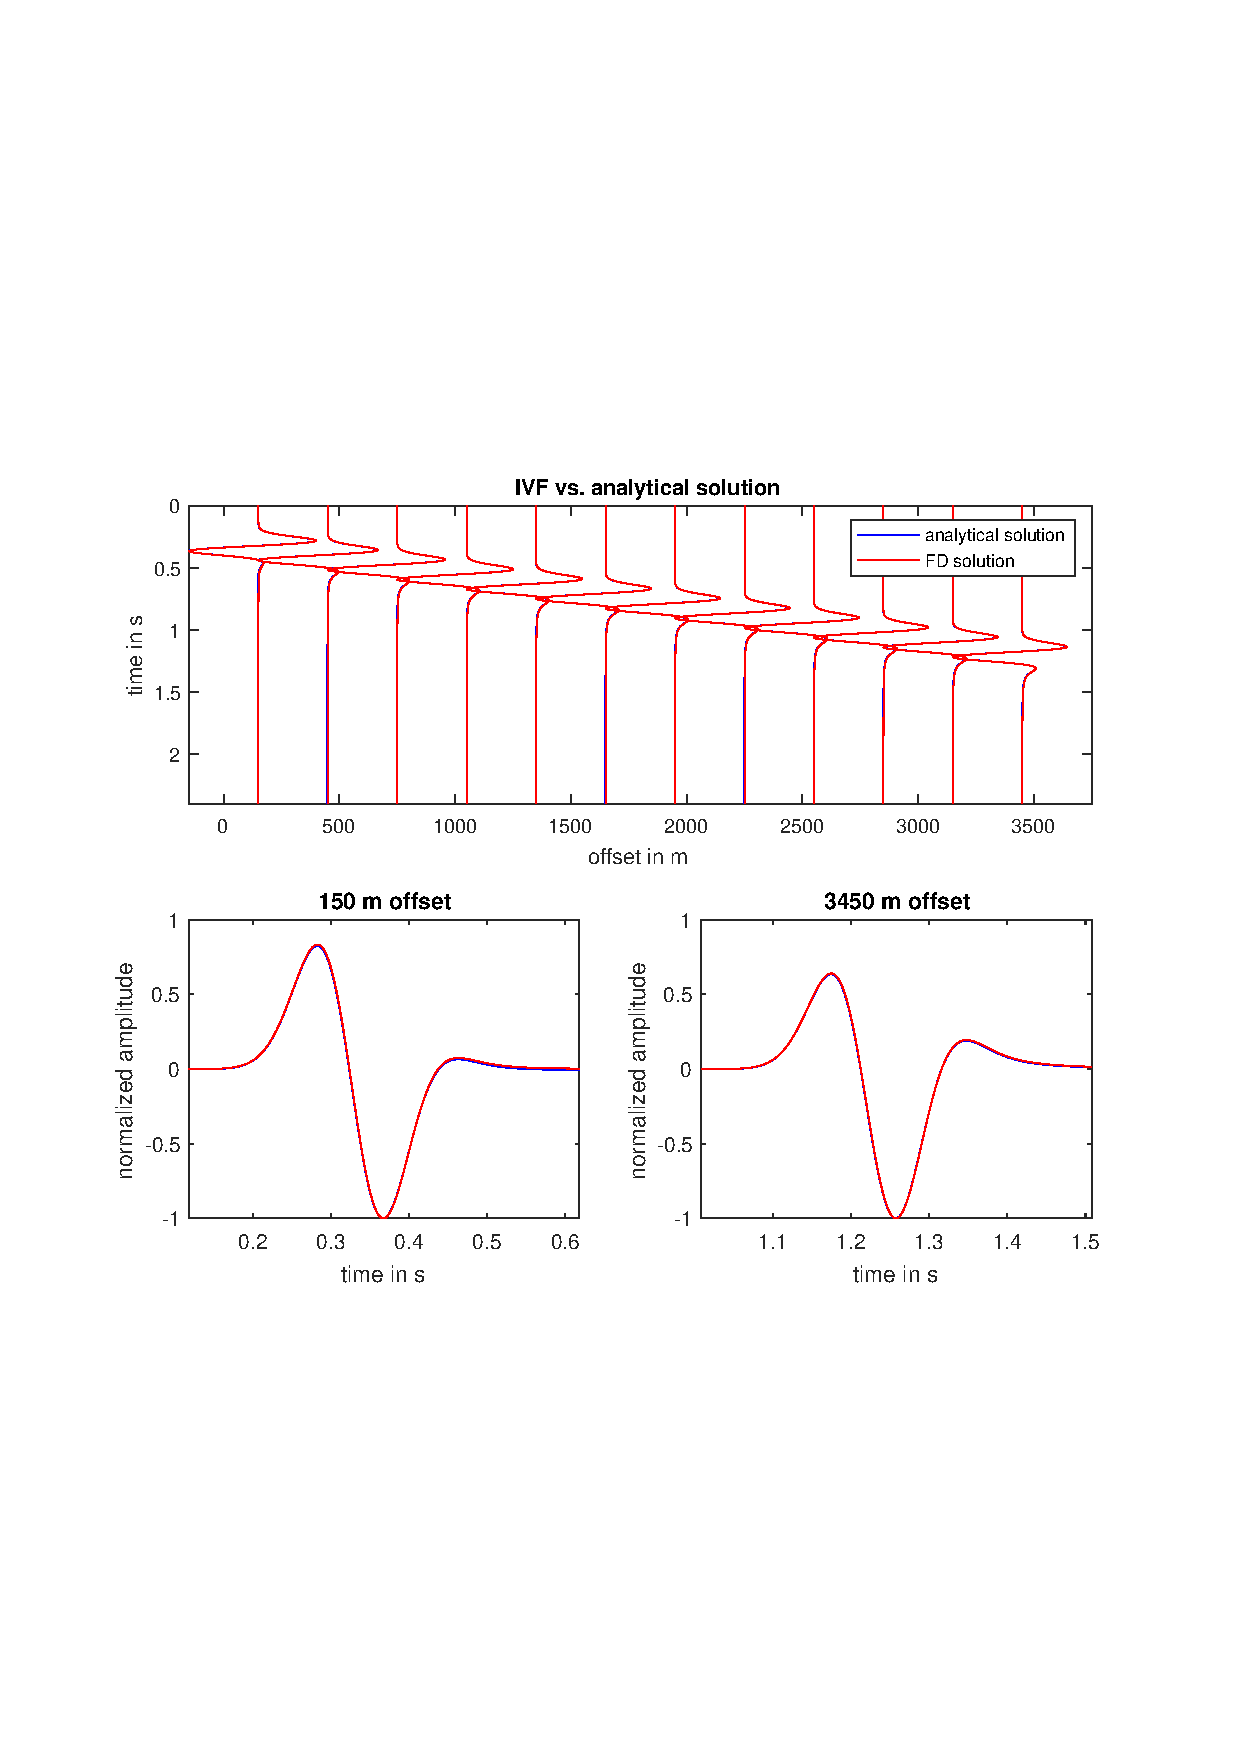
\includegraphics[width=0.7\textwidth,trim=2cm 7cm 2cm 7cm, clip=true]{images/fd_vs_analytic_acoustic_IVF.pdf}
    \caption{Acoustic case. Lower plots show the P-phase at different offsets.}
  \end{subfigure} \\
  \begin{subfigure}[b]{1.0\textwidth}
    \centering
    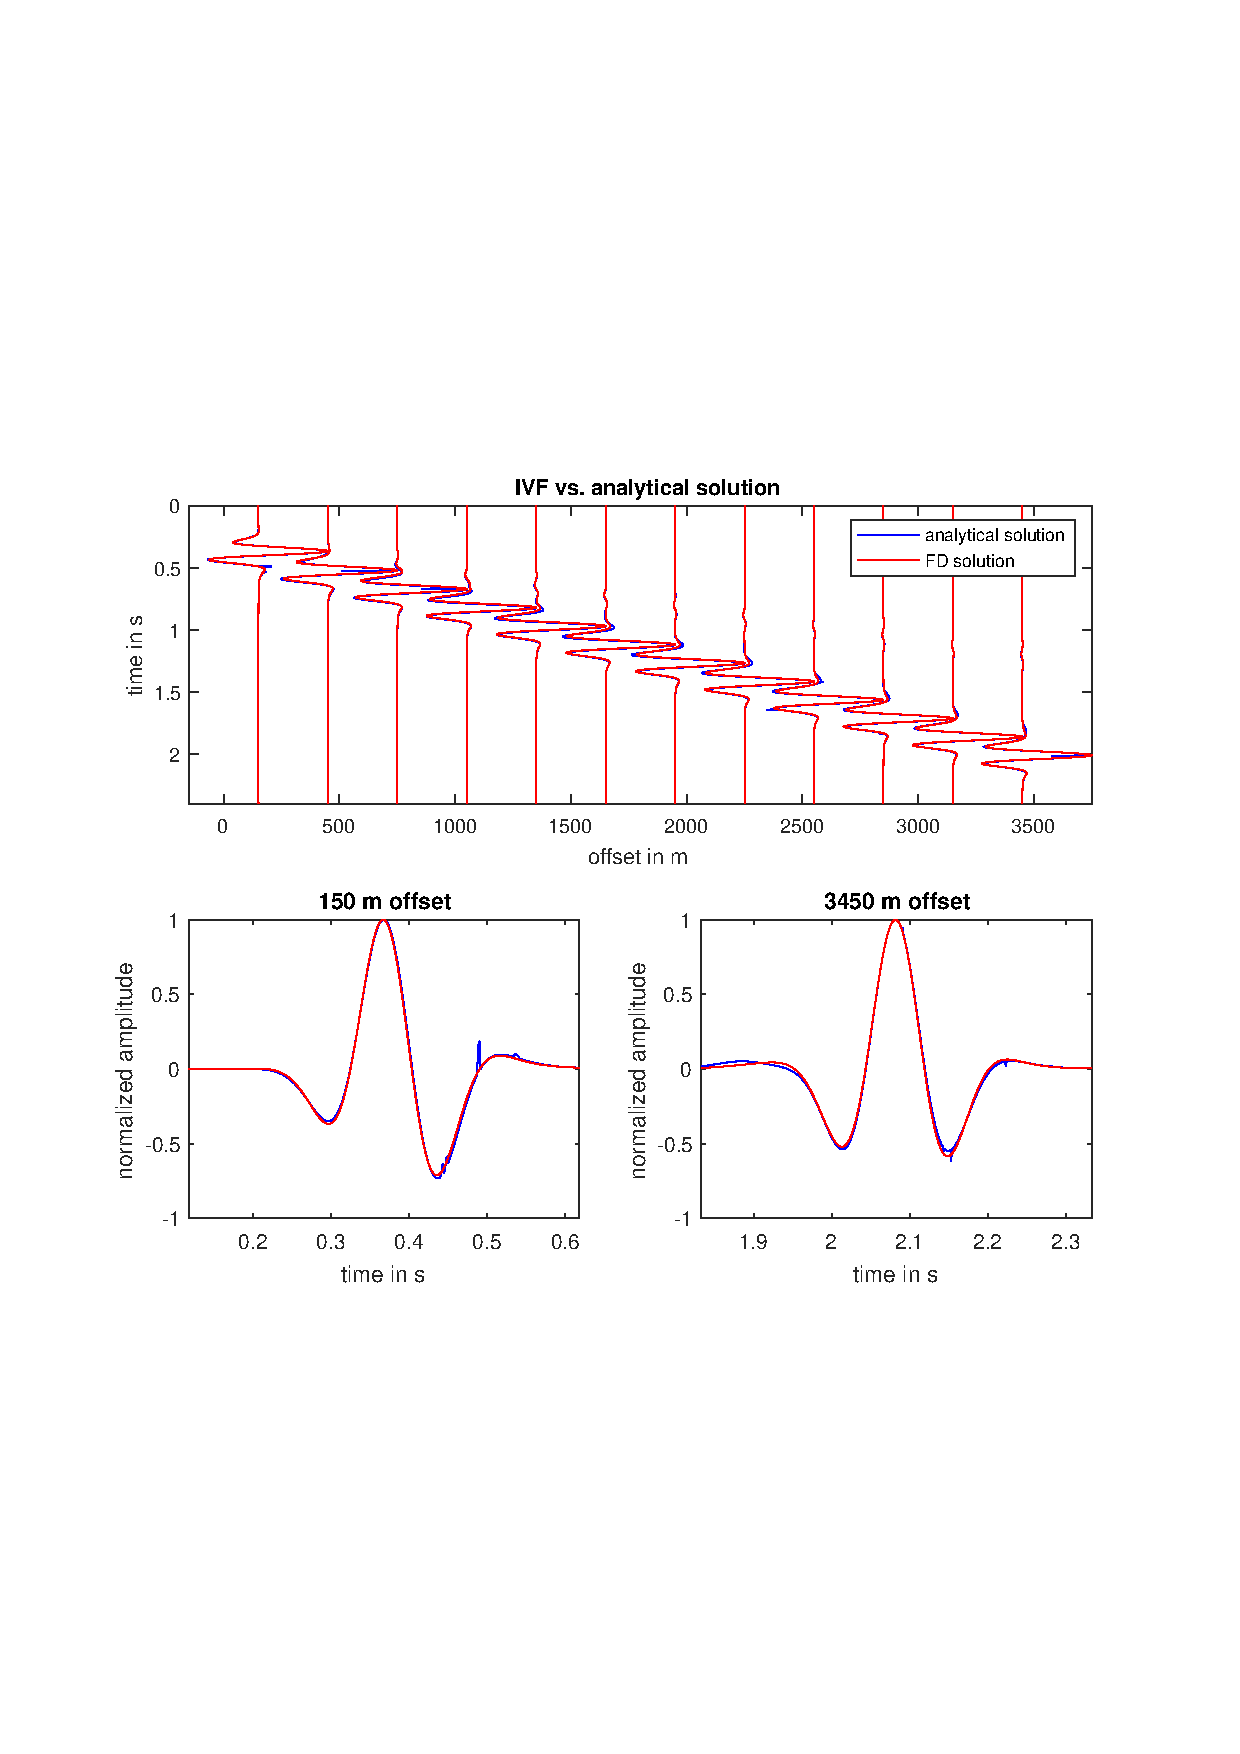
\includegraphics[width=0.7\textwidth,trim=2cm 7cm 2cm 7cm, clip=true]{images/fd_vs_analytic_elastic_IVF.pdf}
    \caption{Elastic case. Lower plots show the Rayleigh wave at different offsets.}
  \end{subfigure} \\
  \caption{Comparison of IVF with the analytic solution. Traces are normalized. The analytic solution shows some numerical instabilities. Sources and receivers are \SI{7.5}{\meter} below the surface.}\label{fig:IVFvsAnalytic}
\end{figure}

\begin{figure}
  \centering
  \begin{subfigure}[b]{1.0\textwidth}
    \centering
    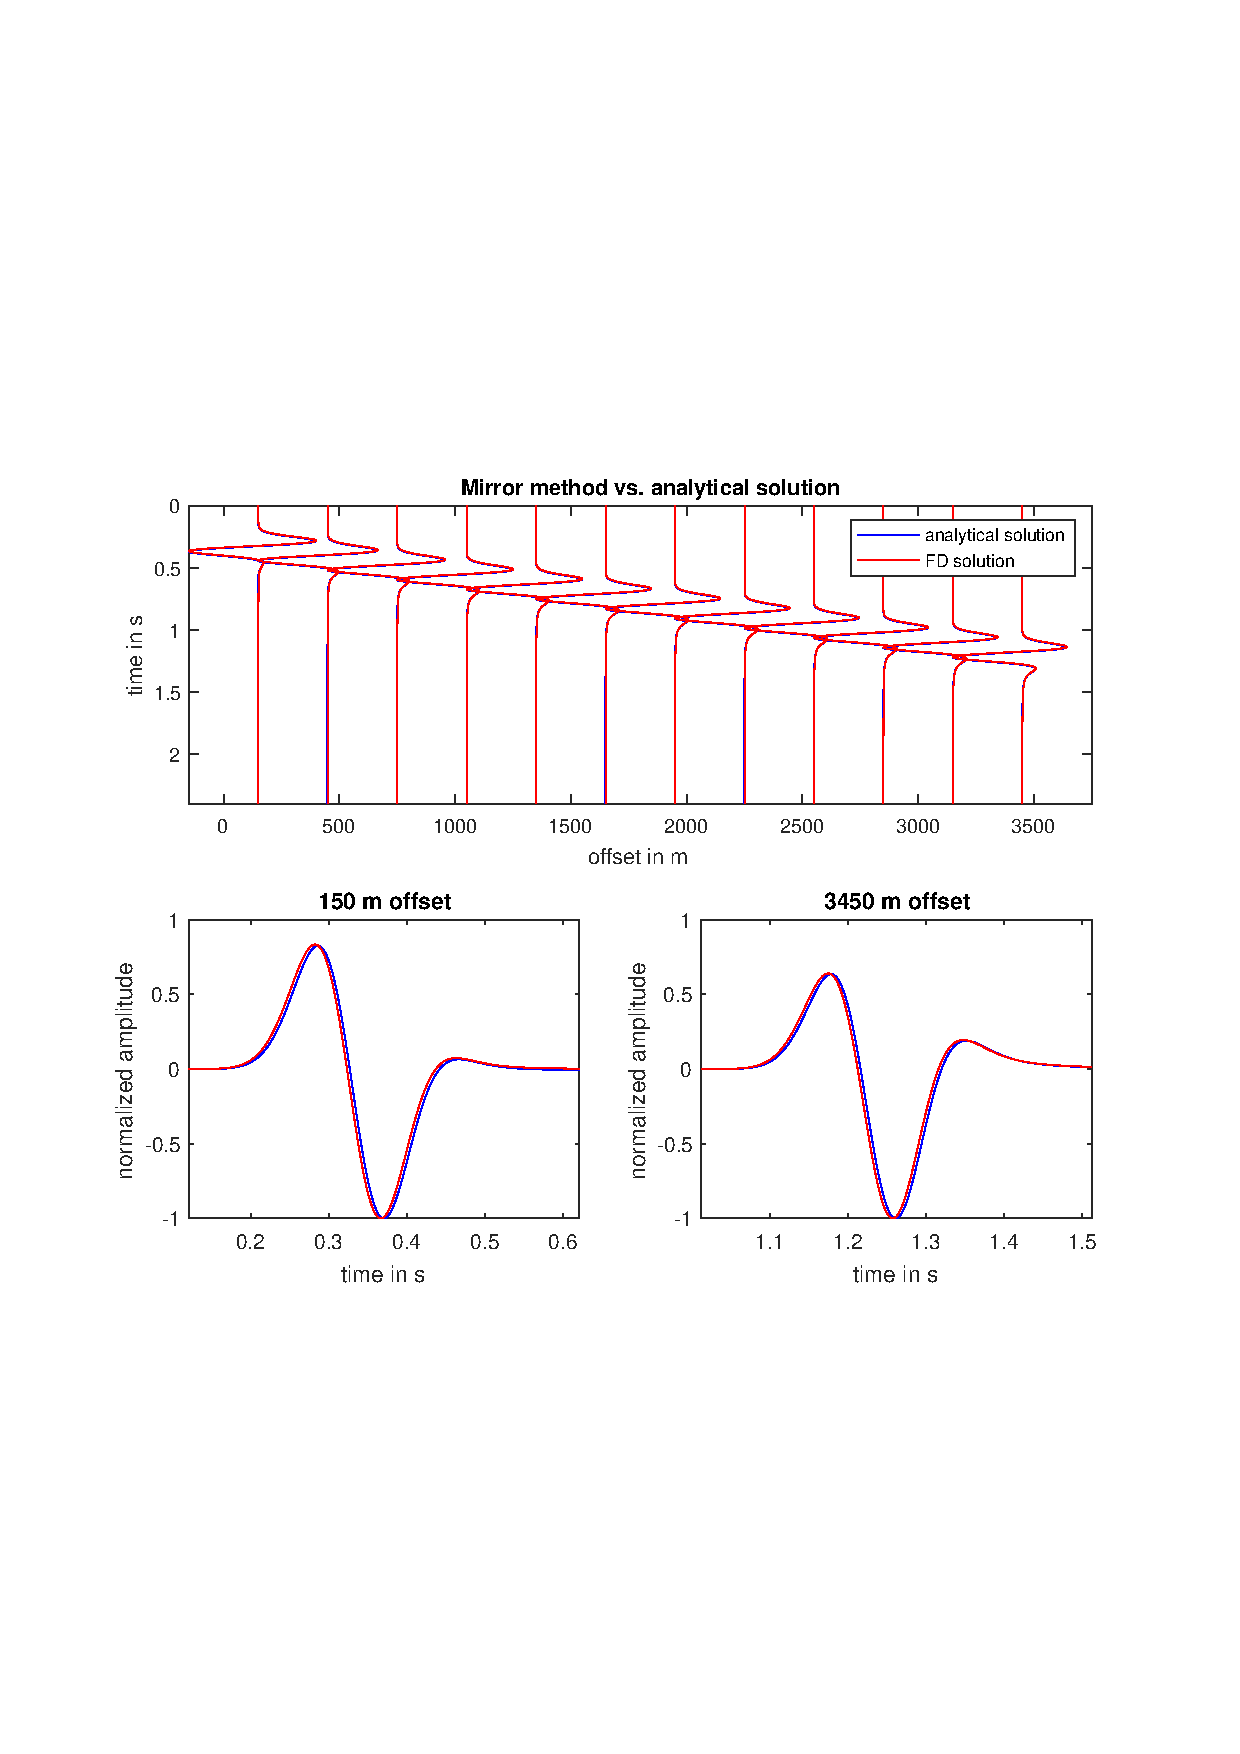
\includegraphics[width=0.7\textwidth,trim=2cm 7cm 2cm 7cm, clip=true]{images/fd_vs_analytic_acoustic_mirror.pdf}
    \caption{Acoustic case. Lower plots show the P-phase at different offsets.}
  \end{subfigure} \\
  \begin{subfigure}[b]{1.0\textwidth}
    \centering
    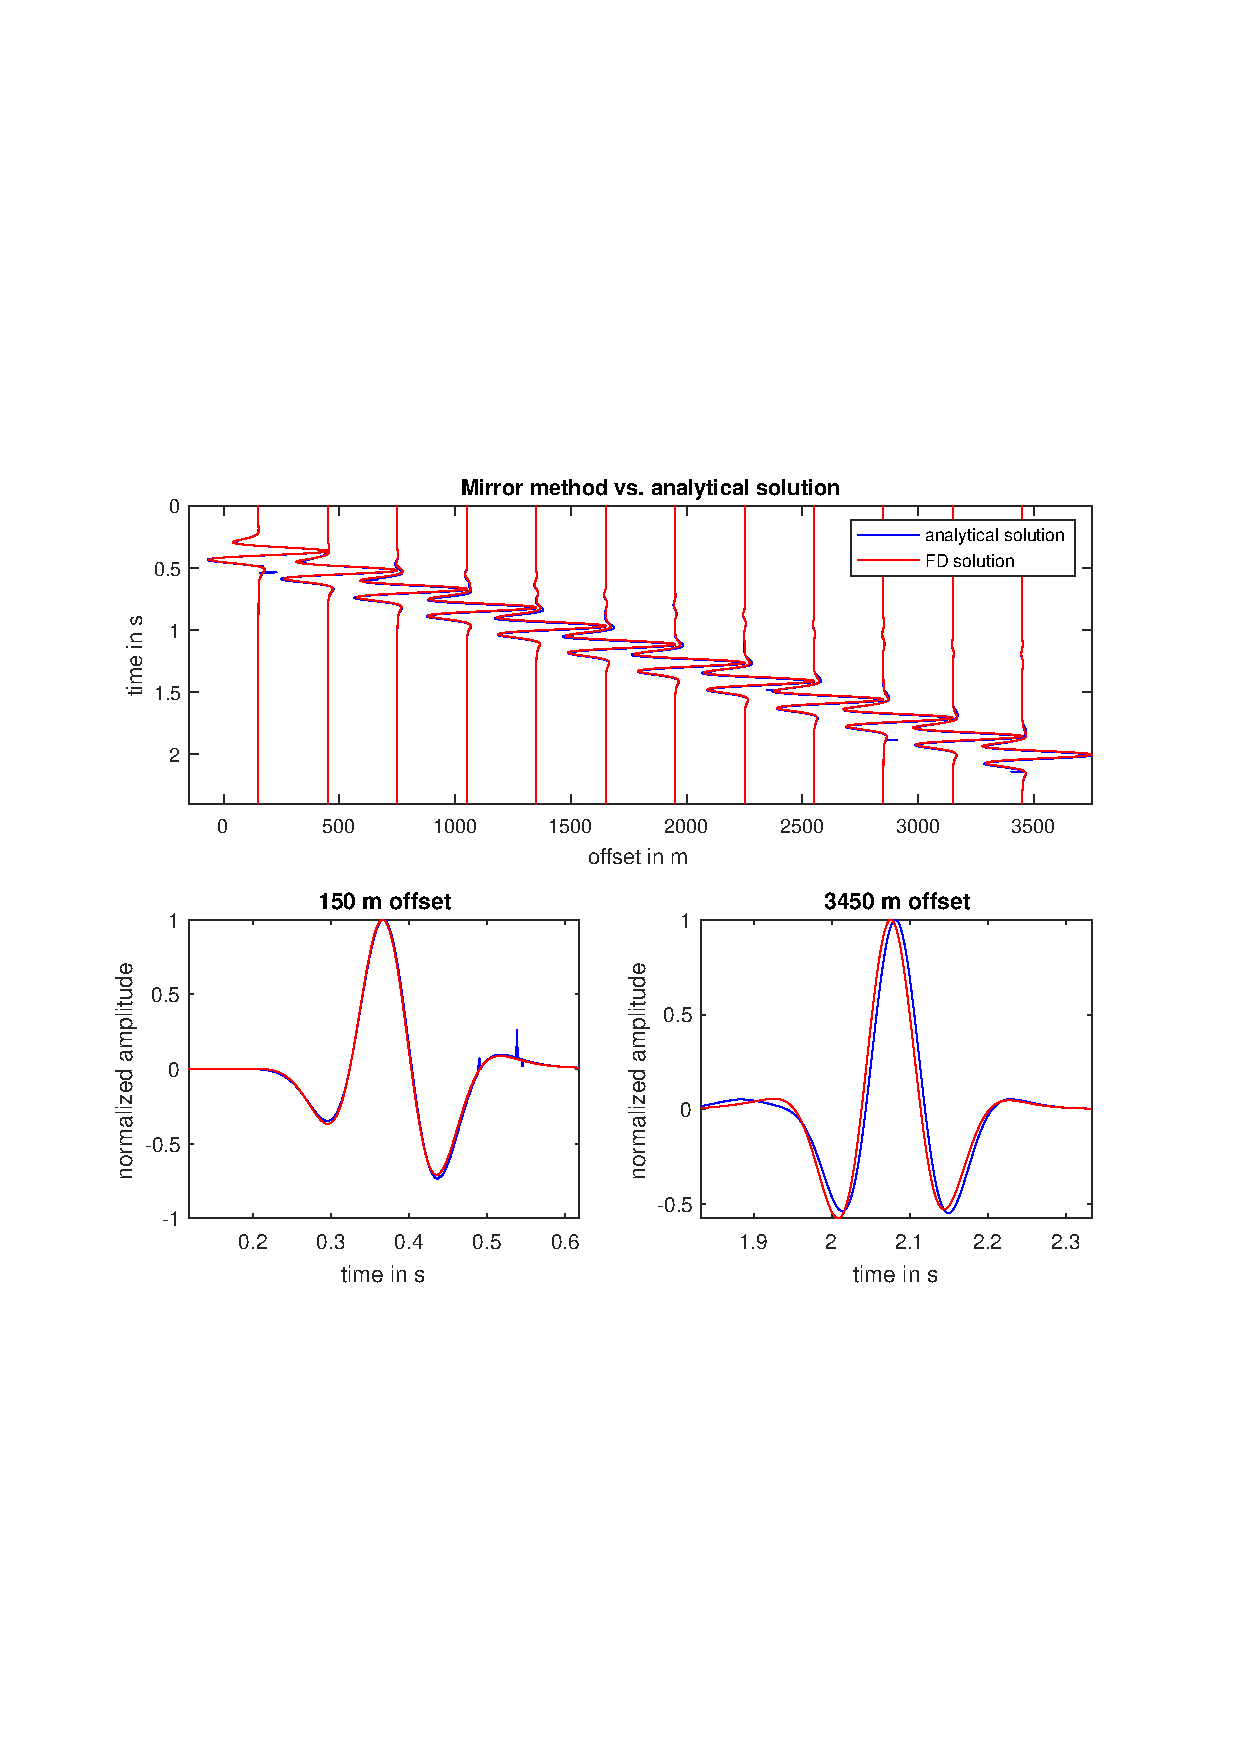
\includegraphics[width=0.7\textwidth,trim=2cm 7cm 2cm 7cm, clip=true]{images/fd_vs_analytic_elastic_mirror.pdf}
    \caption{Elastic case. Lower plots show the Rayleigh wave at different offsets.}
  \end{subfigure} \\
  \caption{Comparison of mirror method with the analytic solution. Traces are normalized. The analytic solution shows some numerical instabilities. Sources and receivers are \SI{3.75}{\meter} below the surface.}\label{fig:MirrorvsAnalytic}
\end{figure}

\cleardoublepage
\addtocontents{toc}{\protect\setcounter{tocdepth}{0}}
\listoffigures 
\addtocontents{toc}{\protect\setcounter{tocdepth}{1}}
\addcontentsline{toc}{chapter}{List of Figures}
\addtocontents{toc}{\protect\setcounter{tocdepth}{0}}
\listoftables
\addtocontents{toc}{\protect\setcounter{tocdepth}{1}}
\addcontentsline{toc}{chapter}{List of Tables}
\cleardoublepage
%\bibliography{@CMAKE_SOURCE_DIR@/../doc/guide/WAVE_Simulation_guide}
\bibliography{WAVE_Simulation_guide}
\bibliographystyle{apalike}

\appendix

\chapter{Acoustic wave equation}
\label{sec:Acoustic_wave_equation}
\section{Theory of acoustic wave equation}
The acoustic wave equations for pressure and velocity.
\begin{align}
\pdv{p}{t} &= \lambda \pdv{v_k}{x_k} \\
\rho\pdv{v_i}{t}&=\pdv{p}{x_i}+ f_i
\end{align}
Note that the pressure, $p$, is defined in an unconventional way as $p=\frac{1}{3}\mathrm{tr}(\sigma_{ij})$. Usually it is defined with a negative sign as $p=-\frac{1}{3}\mathrm{tr}(\sigma_{ij})$.

\section{Discretization of acoustic wave equation}
Derivation of the acoustic wave equations for the SSG in Fig.\ref{fig:StagGrid3D} yields the following system of equations for pressure and velocity. \\
\begin{align*}
	p_{i,j,k}^{n+\frac{1}{2}} &= p_{i,j,k}^{n-\frac{1}{2}} + \Delta t \cdot \lambda_{i,j,k} \left( \left.\frac{\partial v_x}{\partial x}\right\rvert_{i,j,k}^n + \left.\frac{\partial v_y}{\partial y}\right\rvert_{i,j,k}^n + \left.\frac{\partial v_z}{\partial z}\right\rvert_{i,j,k}^n \right)\\
	v_{x,i+\frac{1}{2},j,k}^{n+1} &= v_{x,i+\frac{1}{2},j,k}^n + \frac{\Delta t}{\rho_{i+\frac{1}{2},j,k}} \frac{\partial p}{\partial x} \\
	v_{y,i,j+\frac{1}{2},k}^{n+1} &= v_{y,i,j+\frac{1}{2},k}^n + \frac{\Delta t}{\rho_{i,j+\frac{1}{2},k}} \frac{\partial p}{\partial y} \\
	v_{z,i,j,k+\frac{1}{2}}^{n+1} &= v_{z,i,j,k+\frac{1}{2}}^n + \frac{\Delta t}{\rho_{i,j,k+\frac{1}{2}}} \frac{\partial p}{\partial z}
\end{align*}

\section{Matrix-vector formalism of acoustic wave equation}
The discrete components for an acoustic wavefield in matrix-vector notation can be written as following. 
\begin{align*}
	\vec{p}^{\,n} &= \vec{p}^{\,n-1} + \frac{\Delta t}{\Delta h}~ \mathrm{diag} \left( \vec{\lambda}^{\,T} \right) \cdot \left( \underline{D}_{\,x,b}^q \vec{v}_x^{\,n} +\underline{D}_{\,y,b}^q \vec{v}_y^{\,n} + \underline{D}_{\,z,b}^q \vec{v}_z^{\,n} \right) \\
	\vec{v}_x^{\,n+1} &= \vec{v}_x^{\,n} + \frac{\Delta t}{\Delta h} ~ \mathrm{diag} \left( \vec{\rho}_{x,\mathrm{inv}}^{\,T} \right) \cdot \left( \underline{D}_{\,x,f}^q \vec{p}^{\,n}  \right)\\
	\vec{v}_y^{\,n+1} &= \vec{v}_y^{\,n} + \frac{\Delta t}{\Delta h} ~ \mathrm{diag} \left( \vec{\rho}_{y,\mathrm{inv}}^{\,T} \right) \cdot \left( \underline{D}_{\,y,f}^q \vec{p}^{\,n} \right)\\
	\vec{v}_z^{\,n+1} &= \vec{v}_z^{\,n} + \frac{\Delta t}{\Delta h} ~ \mathrm{diag}  \left( \vec{\rho}_{z,\mathrm{inv}}^{\,T} \right) \cdot\left( \underline{D}_{\,z,f}^q \vec{p}^{\,n} \right)\\
\end{align*}

\chapter{Viscoelastic wave equation}
\label{sec:Viscoelastic_wave_equation}

\section{Theory of viscoelastic wave equation}
The viscoelastic wave equations for stress and velocity \citep{bohlen2002parallel}.
\begin{align}
\label{eqn:elastic_wave_stress_xx}
\pdv{\sigma_{ii}}{t} &= \left\{ \pi (1+\tau^p)-2\mu (1+\tau^s) \right\} \pdv{v_k}{x_k} + 2\mu (1+\tau^s) \pdv{v_i}{x_i} + \sum_{l=1}^L r_{iil}\\
\pdv{\sigma_{ij}}{t} &= \mu (1+\tau^s) \left(\pdv{v_i}{x_j} +\pdv{v_j}{x_i}\right) + \sum_{l=1}^L r_{ijl}, \quad i \neq j\\
\rho\pdv{v_i}{t}&=\pdv{\sigma_{ij}}{x_j}+ f_i
\end{align}
with the so-called memory equations:
\begin{align}
\pdv{r_{iil}}{t} &= -\frac{1}{\tau_{\sigma l}} \left\{ (\pi \tau^p-2\mu \tau^s) \pdv{v_k}{x_k} + 2\mu \tau^s \pdv{v_i}{x_i} + r_{iil} \right\}\\
\pdv{r_{ijl}}{t} &= -\frac{1}{\tau_{\sigma l}} \left\{ \mu (1+\tau^s) \left(\pdv{v_i}{x_j} +\pdv{v_j}{x_i}\right) + r_{ijl} \right\}, \quad i \neq j
\end{align}

\section{Discretization of viscoelastic wave equation}
Derivation of the viscoelastic wave equations for the SSG in Fig.\ref{fig:StagGrid3D} yields the following system of equations for stress and velocity. \\
The components of the stress tensor are given by:
\begin{align*}
	\sigma_{xx,i,j,k}^{n+\frac{1}{2}} =& \;\sigma_{xx,i,j,k}^{n-\frac{1}{2}}+ \Bigg[ \Delta t \cdot \pi_{i,j,k} \left(1+L\cdot \tau^p_{i,j,k}\right)\left( \left.\frac{\partial v_x}{\partial x}\right\rvert_{i,j,k}^{n} + \left.\frac{\partial v_y}{\partial y}\right\rvert_{i,j,k}^{n} + \left.\frac{\partial v_z}{\partial z}\right\rvert_{i,j,k}^{n} \right)\Bigg]  \\
	&- \Bigg[ 2 \Delta t \cdot \mu_{i,j,k} \left(1+L\cdot \tau^s_{i,j,k}\right)\cdot \left( \left.\frac{\partial v_y}{\partial y}\right\rvert_{i,j,k}^{n} + \left.\frac{\partial v_z}{\partial z}\right\rvert_{i,j,k}^{n} \right)\Bigg] \\
	&+ \frac{\Delta t}{2} \sum _{l=1}^{L} \left( r_{xx,l,i,j,k}^{n-\frac{1}{2}}+ r_{xx,l,i,j,k}^{n+\frac{1}{2}}\right) \\
	\sigma_{yy,i,j,k}^{n+\frac{1}{2}} =&\;\sigma_{yy,i,j,k}^{n}+ \Bigg[ \Delta t \cdot \pi_{i,j,k} \left(1+L\cdot \tau^p_{i,j,k}\right)\left( \left.\frac{\partial v_x}{\partial x}\right\rvert_{i,j,k}^{n} + \left.\frac{\partial v_y}{\partial y}\right\rvert_{i,j,k}^{n} + \left.\frac{\partial v_z}{\partial z}\right\rvert_{i,j,k}^{n} \right)\Bigg]  \\
	&- \Bigg[ 2 \Delta t \cdot \mu_{i,j,k} \left(1+L\cdot \tau^s_{i,j,k}\right)\cdot \left( \left.\frac{\partial v_x}{\partial x}\right\rvert_{i,j,k}^{n} + \left.\frac{\partial v_z}{\partial z}\right\rvert_{i,j,k}^{n-} \right)\Bigg] \\
	&+ \frac{\Delta t}{2} \sum _{l=1}^{L} \left( r_{yy,l,i,j,k}^{n-\frac{1}{2}}+ r_{yy,l,i,j,k}^{n+\frac{1}{2}}\right)\\ 
	\sigma_{zz,i,j,k}^{n+\frac{1}{2}} =&\;\sigma_{zz,i,j,k}^{n-\frac{1}{2}}+ \Bigg[ \Delta t \cdot \pi_{i,j,k} \left(1+L\cdot \tau^p_{i,j,k}\right)\left( \left.\frac{\partial v_x}{\partial x}\right\rvert_{i,j,k}^{n}+ \left.\frac{\partial v_y}{\partial y}\right\rvert_{i,j,k}^{n} + \left.\frac{\partial v_z}{\partial z}\right\rvert_{i,j,k}^{n} \right)\Bigg]  \\
	&- \Bigg[ 2 \Delta t \cdot \mu_{i,j,k} \left(1+L\cdot \tau^s_{i,j,k}\right)\cdot \left( \left.\frac{\partial v_x}{\partial x}\right\rvert_{i,j,k}^{n} + \left.\frac{\partial v_y}{\partial y}\right\rvert_{i,j,k}^{n} \right)\Bigg] \\
	&+ \frac{\Delta t}{2} \sum _{l=1}^{L} \left( r_{yy,l,i,j,k}^{n-\frac{1}{2}}+ r_{yy,l,i,j,k}^{n+\frac{1}{2}}\right)\\ 
	\sigma_{xy,i+\frac{1}{2},j+\frac{1}{2},k}^{n+\frac{1}{2}} =&\;\sigma_{xy,i+\frac{1}{2},j+\frac{1}{2},k}^{n-\frac{1}{2}}+\Bigg[\Delta t \cdot \mu_{i+\frac{1}{2},j+\frac{1}{2},k}\left(1+L\cdot\tau_{i+\frac{1}{2},j+\frac{1}{2},k}^s \right)\cdot \\ 
	&\left( \left.\frac{\partial v_x}{\partial y}\right\rvert_{i+\frac{1}{2},j+\frac{1}{2},k}^n + \left.\frac{\partial v_y}{\partial x}\right\rvert_{i+\frac{1}{2},j+\frac{1}{2},k}^n \right)\Bigg] + \frac{\Delta t}{2} \sum _{l=1}^{L} \left( r_{xy,l,i+\frac{1}{2},j+\frac{1}{2},k}^{n-\frac{1}{2}}+ r_{xy,l,i+\frac{1}{2},j+\frac{1}{2},k}^{n+\frac{1}{2}}\right) \\
	\sigma_{xz,i+\frac{1}{2},j,k+\frac{1}{2}}^{n+\frac{1}{2}} =&\;\sigma_{xy,i+\frac{1}{2},j,k+\frac{1}{2}}^{n-\frac{1}{2}}+\Bigg[\Delta t \cdot \mu_{i+\frac{1}{2},j,k+\frac{1}{2}}\left(1+L\cdot\tau_{i+\frac{1}{2},j,k+\frac{1}{2}}^s \right)\cdot \\ 
	&\left( \left.\frac{\partial v_x}{\partial y}\right\rvert_{i+\frac{1}{2},j,k+\frac{1}{2}}^n + \left.\frac{\partial v_y}{\partial x}\right\rvert_{i+\frac{1}{2},j,k+\frac{1}{2}}^n \right)\Bigg]  + \frac{\Delta t}{2} \sum _{l=1}^{L} \left( r_{xy,l,i+\frac{1}{2},j,k+\frac{1}{2}}^{n-\frac{1}{2}}+ r_{xy,l,i+\frac{1}{2},j,k+\frac{1}{2}}^{n+\frac{1}{2}}\right) \\
	\sigma_{yz,i,j+\frac{1}{2},k+\frac{1}{2}}^{n+\frac{1}{2}} =& \;\sigma_{xy,i,j+\frac{1}{2},k+\frac{1}{2}}^{n-\frac{1}{2}}+\Bigg[\Delta t \cdot \mu_{i,j+\frac{1}{2},k+\frac{1}{2}}\left(1+L\cdot\tau_{i,j+\frac{1}{2},k+\frac{1}{2}}^s \right)\cdot \\ 
	&\left( \left.\frac{\partial v_x}{\partial y}\right\rvert_{i,j+\frac{1}{2},k+\frac{1}{2}}^n + \left.\frac{\partial v_y}{\partial x}\right\rvert_{i,j+\frac{1}{2},k+\frac{1}{2}}^n \right)\Bigg]  + \frac{\Delta t}{2} \sum _{l=1}^{L} \left( r_{xy,l,i,j+\frac{1}{2},k+\frac{1}{2}}^{n-\frac{1}{2}}+ r_{xy,l,i,j+\frac{1}{2},k+\frac{1}{2}}^{n+\frac{1}{2}}\right) \\
\end{align*}
\begin{align*}
	r_{xx,l,i,j,k}^{n+\frac{1}{2}} =& \left( 1+ \frac{\Delta t}{2\tau_{\sigma,l}} \right)^{-1}\cdot \Bigg[\left( 1- \frac{\Delta t}{2\tau_{\sigma,l}}  \right) \cdot r_{xx,l,i,j,k}^{n-\frac{1}{2}} \\ 
	& -\frac{\pi_{i,j,k}\cdot\Delta t}{\tau_{\sigma,l}}\cdot \tau^p_{i,j,k} \cdot \left( \left.\frac{\partial v_x}{\partial x}\right\rvert_{i,j,k}^{n} + \left.\frac{\partial v_y}{\partial y}\right\rvert_{i,j,k}^{n} + \left.\frac{\partial v_z}{\partial z}\right\rvert_{i,j,k}^{n} \right)\\
	& + \frac{2\mu_{i,j,k} \Delta t}{\tau_{\sigma,l}}\cdot \tau^s_{i,j,k} \left( \left.\frac{\partial v_y}{\partial y}\right\rvert_{i,j,k}^{n} + \left.\frac{\partial v_z}{\partial z}\right\rvert_{i,j,k}^{n}  \right)\Bigg] \\
	r_{yy,l,i,j,k}^{n+\frac{1}{2}} =& \left( 1+ \frac{\Delta t}{2\tau_{\sigma,l}} \right)^{-1}\cdot \Bigg[\left( 1- \frac{\Delta t}{2\tau_{\sigma,l}}  \right) \cdot r_{yy,l,i,j,k}^{n-\frac{1}{2}} \\ 
	& -\frac{\pi_{i,j,k}\cdot\Delta t}{\tau_{\sigma,l}}\cdot \tau^p_{i,j,k} \cdot \left( \left.\frac{\partial v_x}{\partial x}\right\rvert_{i,j,k}^{n} + \left.\frac{\partial v_y}{\partial y}\right\rvert_{i,j,k}^{n} + \left.\frac{\partial v_z}{\partial z}\right\rvert_{i,j,k}^{n} \right)\\
	& + \frac{2\mu_{i,j,k} \Delta t}{\tau_{\sigma,l}}\cdot \tau^s_{i,j,k} \left( \left.\frac{\partial v_x}{\partial x}\right\rvert_{i,j,k}^{n} + \left.\frac{\partial v_z}{\partial z}\right\rvert_{i,j,k}^{n}  \right)\Bigg] \\
	r_{zz,l,i,j,k}^{n+\frac{1}{2}} =& \left( 1+ \frac{\Delta t}{2\tau_{\sigma,l}} \right)^{-1}\cdot \Bigg[\left( 1- \frac{\Delta t}{2\tau_{\sigma,l}}  \right) \cdot r_{zz,l,i,j,k}^{n-\frac{1}{2}} \\ 
	& -\frac{\pi_{i,j,k}\cdot\Delta t}{\tau_{\sigma,l}}\cdot \tau^p_{i,j,k} \cdot \left( \left.\frac{\partial v_x}{\partial x}\right\rvert_{i,j,k}^{n} + \left.\frac{\partial v_y}{\partial y}\right\rvert_{i,j,k}^{n} + \left.\frac{\partial v_z}{\partial z}\right\rvert_{i,j,k}^{n} \right)\\
	& + \frac{2\mu_{i,j,k} \Delta t}{\tau_{\sigma,l}}\cdot \tau^s_{i,j,k} \left( \left.\frac{\partial v_x}{\partial x}\right\rvert_{i,j,k}^{n} + \left.\frac{\partial v_y}{\partial y}\right\rvert_{i,j,k}^{n}  \right)\Bigg] \\
	r_{xy,l,i+\frac{1}{2},j+\frac{1}{2},k}^{n+\frac{1}{2}} =& \left( 1+ \frac{\Delta t}{2\tau_{\sigma,l}} \right)^{-1}\cdot \Bigg[\left( 1- \frac{\Delta t}{2\tau_{\sigma,l}}  \right) \cdot r_{xy,l,i+\frac{1}{2},j+\frac{1}{2},k}^{n-\frac{1}{2}} \\ 
	& -\frac{\mu_{i+\frac{1}{2},j+\frac{1}{2},k}\cdot\Delta t}{\tau_{\sigma,l}}\cdot \tau^s_{i+\frac{1}{2},j+\frac{1}{2},k} \cdot \left( \left.\frac{\partial v_x}{\partial y}\right\rvert_{i+\frac{1}{2},j+\frac{1}{2},k}^{n} + \left.\frac{\partial v_y}{\partial x}\right\rvert_{i+\frac{1}{2},j+\frac{1}{2},k}^{n} \right)\Bigg]\\
	r_{xz,l,i+\frac{1}{2},j,k+\frac{1}{2}}^{n+\frac{1}{2}} =& \left( 1+ \frac{\Delta t}{2\tau_{\sigma,l}} \right)^{-1}\cdot \Bigg[\left( 1- \frac{\Delta t}{2\tau_{\sigma,l}}  \right) \cdot r_{xz,l,i+\frac{1}{2},j,k+\frac{1}{2}}^{n-\frac{1}{2}} \\ 
	& -\frac{\mu_{i+\frac{1}{2},j,k+\frac{1}{2}}\cdot\Delta t}{\tau_{\sigma,l}}\cdot \tau^s_{i+\frac{1}{2},j,k+\frac{1}{2}} \cdot \left( \left.\frac{\partial v_x}{\partial z}\right\rvert_{i+\frac{1}{2},j,k+\frac{1}{2}}^{n} + \left.\frac{\partial v_z}{\partial x}\right\rvert_{i+\frac{1}{2},j,k+\frac{1}{2}}^{n} \right)\Bigg]\\
	r_{yz,l,i,j+\frac{1}{2},k+\frac{1}{2}}^{n+\frac{1}{2}} =& \left( 1+ \frac{\Delta t}{2\tau_{\sigma,l}} \right)^{-1}\cdot \Bigg[\left( 1- \frac{\Delta t}{2\tau_{\sigma,l}}  \right) \cdot r_{yz,l,i,j+\frac{1}{2},k+\frac{1}{2}}^{n-\frac{1}{2}} \\ 
	& -\frac{\mu_{i,j+\frac{1}{2},k+\frac{1}{2}}\cdot\Delta t}{\tau_{\sigma,l}}\cdot \tau^s_{i,j+\frac{1}{2},k+\frac{1}{2}} \cdot \left( \left.\frac{\partial v_y}{\partial z}\right\rvert_{i,j+\frac{1}{2},k+\frac{1}{2}}^{n} + \left.\frac{\partial v_z}{\partial y}\right\rvert_{i,j+\frac{1}{2},k+\frac{1}{2}}^{n} \right)\Bigg] \\
\end{align*}
Just as in the elastic case, the velocity equations for the viscoelastic case are given by:
\begin{align*}
	v_{x,i+\frac{1}{2},j,k}^{n+1} &= v_{x,i+\frac{1}{2},j,k}^n + \frac{\Delta t}{\rho_{i+\frac{1}{2},j,k}}  \left( \left.\frac{\partial\sigma_{xx}}{\partial x}\right\rvert_{i+\frac{1}{2},j,k}^{n+\frac{1}{2}} + \left.\frac{\partial\sigma_{xy}}{\partial y}\right\rvert_{i+\frac{1}{2},j,k}^{n+\frac{1}{2}} + \left.\frac{\partial\sigma_{xz}}{\partial z}\right\rvert_{i+\frac{1}{2},j,k}^{n+\frac{1}{2}} \right)\\
	v_{y,i,j+\frac{1}{2},k}^{n+1} &= v_{y,i,j+\frac{1}{2},k}^n + \frac{\Delta t}{\rho_{i,j+\frac{1}{2},k}}  \left( \left.\frac{\partial\sigma_{yx}}{\partial x}\right\rvert_{i,j+\frac{1}{2},k}^{n+\frac{1}{2}} + \left.\frac{\partial\sigma_{yy}}{\partial y}\right\rvert_{i,j+\frac{1}{2},k}^{n+\frac{1}{2}} + \left.\frac{\partial\sigma_{yz}}{\partial z}\right\rvert_{i,j+\frac{1}{2},k}^{n+\frac{1}{2}} \right)\\
	v_{z,i,j,k+\frac{1}{2}}^{n+1} &= v_{z,i,j,k+\frac{1}{2}}^n + \frac{\Delta t}{\rho_{i,j,k+\frac{1}{2}}}  \left( \left.\frac{\partial\sigma_{zx}}{\partial x}\right\rvert_{i,j,k+\frac{1}{2}}^{n+\frac{1}{2}} + \left.\frac{\partial\sigma_{zy}}{\partial y}\right\rvert_{i,j,k+\frac{1}{2}}^{n+\frac{1}{2}} + \left.\frac{\partial\sigma_{zz}}{\partial z}\right\rvert_{i,j,k+\frac{1}{2}}^{n+\frac{1}{2}} \right)
\end{align*}
Here $\mu_{i,j,k}$ is the second Lam\'{e} parameter or S-wave modulus and $\pi_{i,j,k}$ is the P-wave modulus.
The S- and P-wave moduli are defined as:
\begin{align}
	\mu_{i,j,k}&= \rho_{i,j,k}\cdot v_{s,i,j,k}^{2}\\
	\pi_{i,j,k} &= \rho_{i,j,k}\cdot v_{p,i,j,k}^{2}
\end{align}
where $v_{s,i,j,k}$ is the velocity of the S-wave and $v_{p,i,j,k}$ is the velocity of the P-wave.
As the system is represented by relaxation bodies the summation over $l$ is equal to the summation over all $L$ Maxwell-bodies. $\tau_{\sigma,l}$ describes the stress relaxation time and $\tau^s_{i,j,k}$ and $\tau^p_{i,j,k}$ respectively describe the level of attenuation for S- and P-waves. $\tau^s$ on the center of planes is calculated by averaging $\tau^s_{i,j,k}$  from the four surrounding grid points. 
\begin{align*}
	\tau^s_{xy} &= \tau^s_{i+\frac{1}{2},j+\frac{1}{2},k} = \frac{\tau^s_{i,j,k} + \tau^s_{i+1,j,k} + \tau^s_{i,j+1,k} + \tau^s_{i+1,j+1,k}}{4}\\
	\tau^s_{xz} &= \tau^s_{i+\frac{1}{2},j,k+\frac{1}{2}} = \frac{\tau^s_{i,j,k} + \tau^s_{i+1,j,k} + \tau^s_{i,j,k+1} + \tau^s_{i+1,j,k+1}}{4}\\
	\tau^s_{yz} &= \tau^s_{i,j+\frac{1}{2},k+\frac{1}{2}} = \frac{\tau^s_{i,j,k} + \tau^s_{i,j+1,k} + \tau^s_{i,j,k+1} + \tau^s_{i,j+1,k+1}}{4}
\end{align*}
Further on $r_{ij,l}^{n}$ can be interpreted as a memory variable for the $l$-th relaxation body, to help calculating the corresponding stress-tensor component $\sigma_{ij,l}$.

\section{Matrix-vector formalism of viscoelastic wave equation}
All discrete components of the viscoelastic wavefield in matrix-vector notation are: 
\begin{align*}
	\vec{\sigma}_{xx}^{\,n} =& \vec{\sigma}_{xx}^{\,n-1} + \frac{\Delta t}{\Delta h}~ \mathrm{diag} \left[ \vec{\pi}^{\,T} (1+\vec{\tau^p}^{T}) \right] \cdot \left( \underline{D}_{\,x,b}^q \vec{v}_x^{\,n} +\underline{D}_{\,y,b}^q \vec{v}_y^{\,n} + \underline{D}_{\,z,b}^q \vec{v}_z^{\,n} \right) \\
	&- 2~ \frac{\Delta t}{\Delta h} ~\mathrm{diag} \left[ \vec{\mu}^{\,T} (1+\vec{\tau^s}^{T}) \right] \cdot \left( \underline{D}_{\,y,b}^q \vec{v}_y^{\,n} + \underline{D}_{\,z,b}^q \vec{v}_z^{\,n} \right) + \frac{\Delta t}{2} \sum_{l=1}^L \left( \vec{r}_{xxl}^{\,n} + \vec{r}_{xxl}^{\,n-1} \right)\\
	\vec{\sigma}_{yy}^{\,n} =& \vec{\sigma}_{yy}^{\,n-1} + \frac{\Delta t}{\Delta h}~ \mathrm{diag} \left[ \vec{\pi}^{\,T} (1+\vec{\tau^p}^{T}) \right] \cdot \left( \underline{D}_{\,x,b}^q \vec{v}_x^{\,n} +\underline{D}_{\,y,b}^q \vec{v}_y^{\,n} + \underline{D}_{\,z,b}^q \vec{v}_z^{\,n} \right) \\
	&- 2~ \frac{\Delta t}{\Delta h} ~\mathrm{diag} \left[ \vec{\mu}^{\,T} (1+\vec{\tau^s}^{T}) \right] \cdot \left( \underline{D}_{\,x,b}^q \vec{v}_x^{\,n} + \underline{D}_{\,z,b}^q \vec{v}_z^{\,n} \right) + \frac{\Delta t}{2} \sum_{l=1}^L \left( \vec{r}_{yyl}^{\,n} + \vec{r}_{yyl}^{\,n-1} \right)\\
	\vec{\sigma}_{zz}^{\,n} =& \vec{\sigma}_{zz}^{\,n-1} + \frac{\Delta t}{\Delta h}~ \mathrm{diag} \left[ \vec{\pi}^{\,T} (1+\vec{\tau^p}^{T}) \right] \cdot \left( \underline{D}_{\,x,b}^q \vec{v}_x^{\,n} +\underline{D}_{\,y,b}^q \vec{v}_y^{\,n} + \underline{D}_{\,z,b}^q \vec{v}_z^{\,n} \right) \\
	&- 2~ \frac{\Delta t}{\Delta h} ~\mathrm{diag} \left[ \vec{\mu}^{\,T} (1+\vec{\tau^s}^{T}) \right] \cdot \left( \underline{D}_{\,x,b}^q \vec{v}_x^{\,n} + \underline{D}_{\,y,b}^q \vec{v}_y^{\,n} \right) + \frac{\Delta t}{2} \sum_{l=1}^L \left( \vec{r}_{zzl}^{\,n} + \vec{r}_{zzl}^{\,n-1} \right)\\
\end{align*}
\begin{align*}
	\vec{\sigma}_{xy}^{\,n} &= \vec{\sigma}_{xy}^{\,n-1} + \frac{\Delta t}{\Delta h}~ \mathrm{diag} \left[ \vec{\mu}_{xy}^{\,T} (1+\vec{\tau^s_{xy}}^{T}) \right] \cdot \left( \underline{D}_{\,y,f}^q \vec{v}_x^{\,n} + \underline{D}_{\,x,f}^q \vec{v}_y^{\,n} \right) + \frac{\Delta t}{2} \sum_{l=1}^L \left( \vec{r}_{xyl}^{\,n} + \vec{r}_{xyl}^{\,n-1} \right)\\
	\vec{\sigma}_{xz}^{\,n} &= \vec{\sigma}_{xz}^{\,n-1} + \frac{\Delta t}{\Delta h}~ \mathrm{diag} \left[ \vec{\mu}_{xz}^{\,T} (1+\vec{\tau^s_{xz}}^{T}) \right] \cdot \left( \underline{D}_{\,z,f}^q \vec{v}_x^{\,n} + \underline{D}_{\,x,f}^q \vec{v}_z^{\,n} \right) + \frac{\Delta t}{2} \sum_{l=1}^L \left( \vec{r}_{xzl}^{\,n} + \vec{r}_{xzl}^{\,n-1} \right)\\
	\vec{\sigma}_{yz}^{\,n} &= \vec{\sigma}_{yz}^{\,n-1} + \frac{\Delta t}{\Delta h}~ \mathrm{diag} \left[ \vec{\mu}_{yz}^{\,T} (1+\vec{\tau^s_{yz}}^{T}) \right] \cdot \left( \underline{D}_{\,z,f}^q \vec{v}_y^{\,n} + \underline{D}_{\,y,f}^q \vec{v}_z^{\,n} \right) + \frac{\Delta t}{2} \sum_{l=1}^L \left( \vec{r}_{yzl}^{\,n} + \vec{r}_{yzl}^{\,n-1} \right)
\end{align*}
\begin{align*}
	\vec{r}_{xxl}^{\,n} =& \left( 1+\frac{\Delta t}{2 \tau_{\sigma l}} \right)^{-1} \Bigg[ \left( 1-\frac{\Delta t}{2 \tau_{\sigma l}} \right) \vec{r}_{xxl}^{\,n-1} - \frac{\Delta t}{\tau_{\sigma l} \Delta h }~ \mathrm{diag} \left( \vec{\pi}^{\,T} \vec{\tau^p}^{T} \right) \cdot \left( \underline{D}_{\,x,b}^q \vec{v}_x^{\,n} +\underline{D}_{\,y,b}^q \vec{v}_y^{\,n} + \underline{D}_{\,z,b}^q \vec{v}_z^{\,n} \right) \\
	&+ 2~ \frac{\Delta t}{\tau_{\sigma l} \Delta h} ~\mathrm{diag} \left( \vec{\mu}^{\,T} \vec{\tau^s}^{T} \right) \cdot \left( \underline{D}_{\,y,b}^q \vec{v}_y^{\,n} + \underline{D}_{\,z,b}^q \vec{v}_z^{\,n} \right) \Bigg]\\
	\vec{r}_{yyl}^{\,n} =& \left( 1+\frac{\Delta t}{2 \tau_{\sigma l}} \right)^{-1} \Bigg[ \left( 1-\frac{\Delta t}{2 \tau_{\sigma l}} \right) \vec{r}_{yyl}^{\,n-1} - \frac{\Delta t}{\tau_{\sigma l} \Delta h }~ \mathrm{diag} \left( \vec{\pi}^{\,T} \vec{\tau^p}^{T} \right) \cdot \left( \underline{D}_{\,x,b}^q \vec{v}_x^{\,n} +\underline{D}_{\,y,b}^q \vec{v}_y^{\,n} + \underline{D}_{\,z,b}^q \vec{v}_z^{\,n} \right) \\
	&+ 2~ \frac{\Delta t}{\tau_{\sigma l} \Delta h} ~\mathrm{diag} \left( \vec{\mu}^{\,T} \vec{\tau^s}^{T} \right) \cdot \left( \underline{D}_{\,x,b}^q \vec{v}_x^{\,n} + \underline{D}_{\,z,b}^q \vec{v}_z^{\,n} \right) \Bigg]\\
	\vec{r}_{zzl}^{\,n} =& \left( 1+\frac{\Delta t}{2 \tau_{\sigma l}} \right)^{-1} \Bigg[ \left( 1-\frac{\Delta t}{2 \tau_{\sigma l}} \right) \vec{r}_{zzl}^{\,n-1} - \frac{\Delta t}{\tau_{\sigma l} \Delta h }~ \mathrm{diag} \left( \vec{\pi}^{\,T} \vec{\tau^p}^{T} \right) \cdot \left( \underline{D}_{\,x,b}^q \vec{v}_x^{\,n} +\underline{D}_{\,y,b}^q \vec{v}_y^{\,n} + \underline{D}_{\,z,b}^q \vec{v}_z^{\,n} \right) \\
	&+ 2~ \frac{\Delta t}{\tau_{\sigma l} \Delta h} ~\mathrm{diag} \left( \vec{\mu}^{\,T} \vec{\tau^s}^{T} \right) \cdot \left( \underline{D}_{\,x,b}^q \vec{v}_x^{\,n} + \underline{D}_{\,y,b}^q \vec{v}_y^{\,n} \right) \Bigg]\\
\end{align*}
\begin{align*}
	\vec{r}_{xyl}^{\,n} &= \left( 1+\frac{\Delta t}{2 \tau_{\sigma l}} \right)^{-1} \Bigg[ \left( 1-\frac{\Delta t}{2 \tau_{\sigma l}} \right) \vec{r}_{xyl}^{\,n-1} - \frac{\Delta t}{\tau_{\sigma l} \Delta h} ~\mathrm{diag} \left( \vec{\mu}_{xy}^{\,T} \vec{\tau^s_{xy}}^{T} \right) \cdot \left( \underline{D}_{\,y,f}^q \vec{v}_x^{\,n} + \underline{D}_{\,x,f}^q \vec{v}_y^{\,n} \right) \Bigg]\\
	\vec{r}_{xz}^{\,n} &= \left( 1+\frac{\Delta t}{2 \tau_{\sigma l}} \right)^{-1} \Bigg[ \left( 1-\frac{\Delta t}{2 \tau_{\sigma l}} \right) \vec{r}_{xzl}^{\,n-1} - \frac{\Delta t}{\tau_{\sigma l} \Delta h} ~\mathrm{diag} \left( \vec{\mu}_{xz}^{\,T} \vec{\tau_{xz}^s}^{T} \right) \cdot \left( \underline{D}_{\,z,f}^q \vec{v}_x^{\,n} + \underline{D}_{\,x,f}^q \vec{v}_z^{\,n} \right) \Bigg]\\
	\vec{r}_{yz}^{\,n} &= \left( 1+\frac{\Delta t}{2 \tau_{\sigma l}} \right)^{-1} \Bigg[ \left( 1-\frac{\Delta t}{2 \tau_{\sigma l}} \right) \vec{r}_{yzl}^{\,n-1} - \frac{\Delta t}{\tau_{\sigma l} \Delta h} ~\mathrm{diag} \left( \vec{\mu}_{yz}^{\,T} \vec{\tau_{yz}^s}^{T} \right) \cdot \left( \underline{D}_{\,z,f}^q \vec{v}_y^{\,n} + \underline{D}_{\,y,f}^q \vec{v}_z^{\,n} \right) \Bigg]
\end{align*}
\begin{align*}
	\vec{v}_x^{\,n+1} &= \vec{v}_x^{\,n} + \frac{\Delta t}{\Delta h} ~ \mathrm{diag} \left( \vec{\rho}_{x,\mathrm{inv}}^{\,T} \right) \cdot \left( \underline{D}_{\,x,f}^q \vec{\sigma}_{xx}^{\,n} + \underline{D}_{\,y,b}^q \vec{\sigma}_{xy}^{\,n} + \underline{D}_{\,z,b}^q \vec{\sigma}_{xz}^{\,n} \right)\\
	\vec{v}_y^{\,n+1} &= \vec{v}_y^{\,n} + \frac{\Delta t}{\Delta h} ~ \mathrm{diag} \left( \vec{\rho}_{y,\mathrm{inv}}^{\,T} \right) \cdot \left( \underline{D}_{\,x,b}^q \vec{\sigma}_{yx}^{\,n} + \underline{D}_{\,y,f}^q \vec{\sigma}_{yy}^{\,n} + \underline{D}_{\,z,b}^q \vec{\sigma}_{yz}^{\,n} \right)\\
	\vec{v}_z^{\,n+1} &= \vec{v}_z^{\,n} + \frac{\Delta t}{\Delta h} ~ \mathrm{diag} \left( \vec{\rho}_{z,\mathrm{inv}}^{\,T} \right) \cdot \left( \underline{D}_{\,x,b}^q \vec{\sigma}_{zx}^{\,n} + \underline{D}_{\,y,b}^q \vec{\sigma}_{zy}^{\,n} + \underline{D}_{\,z,f}^q \vec{\sigma}_{zz}^{\,n} \right)\\
\end{align*}

\chapter{EM wave equation}
\label{sec:Visco_EM_wave_equation}

\section{Theory of EM wave equation}
Maxwell equations in non-electric charge field are shown as two rotation equations \citep{irving2006numerical}
\begin{equation}
\label{eqn:EM}
\begin{align*}
&\mu_{m} \pdv{ \mathbf{H}}{t} = -\nabla \times \mathbf{E} \\
&\varepsilon\pdv{ \mathbf{E}}{t} + \sigma_{e}\mathbf{E} + \mathbf{J}_s = \nabla \times \mathbf{H} 
\end{align*}
\end{equation}
where $\mathbf{H}$ and $\mathbf{E}$ are the magnetic field and  electric field. The source current $\mathbf{J}_s$ is injected by the GPR antenna. Without taking the visco-dispersion processes into consideration \citep{qin2020numerical2}, the dielectric permittivity $\varepsilon$, conductivity $\sigma_{e}$ and magnetic permeability $\mu_{m}$ are frequency-independent.

\section{Discretization of EM wave equation}
3D EM wave equation and FD discretization by usage of the SSG in isotropic media Fig.\ref{fig:StagGrid3D} are given as:
\begin{equation}
\begin{align*}
  &\mu_{m} \pdv{H_{x}}{t} = -\pdv{E_z}{y} + \pdv{E_y}{z}\\
  &\mu_{m} \pdv{H_{y}}{t} = -\pdv{E_x}{z} + \pdv{E_z}{x}\\
  &\mu_{m} \pdv{H_{z}}{t} = -\pdv{E_y}{x} + \pdv{E_x}{y}\\
  &\varepsilon \pdv{E_{x}}{t} + \sigma_{e} E_{x} + J_{sx} = \pdv{H_z}{y} - \pdv{H_y}{z}\\
  &\varepsilon \pdv{E_{y}}{t} + \sigma_{e} E_{y} + J_{sy} = \pdv{H_x}{z} - \pdv{H_z}{x}\\
  &\varepsilon \pdv{E_{z}}{t} + \sigma_{e} E_{z} + J_{sz} = \pdv{H_y}{x} - \pdv{H_x}{y}
\end{align*}
\end{equation}
\begin{equation}
\begin{align*}
  &H_{x,i,j+\frac{1}{2},k+\frac{1}{2}}^{n+\frac{1}{2}} = H_{x,i,j+\frac{1}{2},k+\frac{1}{2}}^{n-\frac{1}{2}} + \Delta t \cdot \mu_{myz}^{-1}  \left(- \left.\pdv{ E_{z}}{y}\right\rvert_{i,j+\frac{1}{2},k+\frac{1}{2}}^{n} + \left.\pdv{ E_{y}}{z}\right\rvert_{i,j+\frac{1}{2},k+\frac{1}{2}}^{n} \right)\\
  &H_{y,i+\frac{1}{2},j,k+\frac{1}{2}}^{n+\frac{1}{2}} = H_{y,i+\frac{1}{2},j,k+\frac{1}{2}}^{n-\frac{1}{2}} + \Delta t \cdot \mu_{mxz}^{-1}  \left(- \left.\pdv{ E_{x}}{z}\right\rvert_{i+\frac{1}{2},j,k+\frac{1}{2}}^{n} + \left.\pdv{ E_z}{x}\right\rvert_{i+\frac{1}{2},j,k+\frac{1}{2}}^{n} \right)\\
  &H_{z,i+\frac{1}{2},j+\frac{1}{2},k}^{n+\frac{1}{2}} = H_{z,i+\frac{1}{2},j+\frac{1}{2},k}^{n-\frac{1}{2}} + \Delta t \cdot \mu_{mxy}^{-1}  \left(- \left.\pdv{ E_y}{x}\right\rvert_{i+\frac{1}{2},j+\frac{1}{2},k}^{n} + \left.\pdv{ E_x}{y}\right\rvert_{i+\frac{1}{2},j+\frac{1}{2},k}^{n} \right)\\
  &E_{x,i+\frac{1}{2},j,k}^{n+1} = C_{ax} E_{x,i+\frac{1}{2},j,k}^{n} + \Delta t \cdot C_{bx} \left( \left.\pdv{ H_z}{y}\right\rvert_{i+\frac{1}{2},j,k}^{n+\frac{1}{2}} - \left.\pdv{ H_y}{z}\right\rvert_{i+\frac{1}{2},j,k}^{n+\frac{1}{2}} - J_{sx} \right)\\
  &E_{y,i,j+\frac{1}{2},k}^{n+1} = C_{ay} E_{y,i,j+\frac{1}{2},k}^{n} + \Delta t \cdot C_{by} \left( \left.\pdv{ H_x}{z}\right\rvert_{i,j+\frac{1}{2},k}^{n+\frac{1}{2}} - \left.\pdv{ H_z}{x}\right\rvert_{i,j+\frac{1}{2},k}^{n+\frac{1}{2}} - J_{sy} \right)\\
  &E_{z,i,j,k+\frac{1}{2}}^{n+1} = C_{az} E_{z,i,j,k+\frac{1}{2}}^{n} + \Delta t \cdot C_{bz} \left( \left.\pdv{ H_y}{x}\right\rvert_{i,j,k+\frac{1}{2}}^{n+\frac{1}{2}} - \left.\pdv{ H_x}{y}\right\rvert_{i,j,k+\frac{1}{2}}^{n+\frac{1}{2}} - J_{sz} \right)
\end{align*}
\end{equation}
where
\begin{align*}
  &\mu_{mxy} = \frac{4}{\mu^{-1}_{m,i,j,k} + \mu^{-1}_{m,i+1,j,k} + \mu^{-1}_{m,i,j+1,k} + \mu^{-1}_{m,i+1,j+1,k}}\\
  &\mu_{mxz} = \frac{4}{\mu^{-1}_{m,i,j,k} + \mu^{-1}_{m,i+1,j,k} + \mu^{-1}_{m,i,j,k+1} + \mu^{-1}_{m,i+1,j,k+1}}\\
  &\mu_{myz} = \frac{4}{\mu^{-1}_{m,i,j,k} + \mu^{-1}_{m,i,j+1,k} + \mu^{-1}_{m,i,j,k+1} + \mu^{-1}_{m,i,j+1,k+1}}\\
  &C_{ai} = \left( 1 - \frac{\sigma_{ei} \Delta t}{2 \varepsilon_{i}} \right) \left( 1 + \frac{\sigma_{ei} \Delta t}{2 \varepsilon_{i}} \right)^{-1}, \quad
  C_{bi} = \frac{1}{\varepsilon_{i}} \left( 1 + \frac{\sigma_{ei} \Delta t}{2 \varepsilon_{i}} \right)^{-1}, \quad
  i = x,y,z\\
  &\varepsilon_{x} = \frac{\varepsilon_{i,j,k} + \varepsilon_{i+1,j,k}}{2}, \quad
  \varepsilon_{y} = \frac{\varepsilon_{i,j,k} + \varepsilon_{i,j+1,k}}{2}, \quad
  \varepsilon_{z} = \frac{\varepsilon_{i,j,k} + \varepsilon_{i,j,k+1}}{2} \\
  &\sigma_{ey} = \frac{\sigma_{e,i,j,k} + \sigma_{e,i,j+1,k}}{2}, \quad 
  \sigma_{ex} = \frac{\sigma_{e,i,j,k} + \sigma_{e,i+1,j,k}}{2}, \quad 
  \sigma_{ez} = \frac{\sigma_{e,i,j,k} + \sigma_{e,i,j,k+1}}{2} 
\end{align*}

\section{Matrix-vector formalism of EM wave}
All discrete components of the 3D EM wavefield in matrix-vector notation are: 
\begin{equation}
\begin{align*}
  &\vec{H}_{x}^{n+\frac{1}{2}} = \vec{H}_{x}^{n-\frac{1}{2}} + \frac{\Delta t}{\Delta h} \cdot  \mathrm{diag} \left(\vec{\mu}_{myz}^{-1}\right)  \left(- \underline{D}_{\,y,f}^q \vec{E}_{z}^{n} + \underline{D}_{\,z,f}^q \vec{E}_{y}^{n} \right)\\
  &\vec{H}_{y}^{n+\frac{1}{2}} = \vec{H}_{y}^{n-\frac{1}{2}} + \frac{\Delta t}{\Delta h} \cdot  \mathrm{diag} \left(\vec{\mu}_{mxz}^{-1}\right)  \left(- \underline{D}_{\,z,f}^q \vec{E}_{x}^{n} + \underline{D}_{\,x,f}^q \vec{E}_z^{n} \right)\\
  &\vec{H}_{z}^{n+\frac{1}{2}} = \vec{H}_{z}^{n-\frac{1}{2}} + \frac{\Delta t}{\Delta h} \cdot  \mathrm{diag} \left(\vec{\mu}_{mxy}^{-1}\right)  \left(- \underline{D}_{\,x,f}^q \vec{E}_y^{n} + \underline{D}_{\,y,f}^q \vec{E}_x^{n} \right)\\
  &\vec{E}_{x}^{n+1} =  \mathrm{diag} \left(\vec{C}_{ax}\right) \vec{E}_{x}^{n} + \Delta t \cdot  \mathrm{diag} \left(\vec{C}_{bx}\right) \left[ \frac{1}{\Delta h} \left( \underline{D}_{\,y,b}^q \vec{H}_z^{n+\frac{1}{2}} - \underline{D}_{\,z,b}^q \vec{H}_y^{n+\frac{1}{2}} \right) - J_{sx} \right]\\
  &\vec{E}_{y}^{n+1} =  \mathrm{diag} \left(\vec{C}_{ay}\right) \vec{E}_{y}^{n} + \Delta t \cdot  \mathrm{diag} \left(\vec{C}_{by}\right) \left[ \frac{1}{\Delta h} \left( \underline{D}_{\,z,b}^q  \vec{H}_x^{n+\frac{1}{2}} - \underline{D}_{\,x,b}^q \vec{H}_z^{n+\frac{1}{2}} \right) - J_{sy} \right]\\
  &\vec{E}_{z}^{n+1} =  \mathrm{diag} \left(\vec{C}_{az}\right) \vec{E}_{z}^{n} + \Delta t \cdot  \mathrm{diag} \left(\vec{C}_{bz}\right) \left[ \frac{1}{\Delta h} \left( \underline{D}_{\,x,b}^q \vec{H}_y^{n+\frac{1}{2}} - \underline{D}_{\,y,b}^q \vec{H}_x^{n+\frac{1}{2}} \right) - J_{sz} \right]
\end{align*}
\end{equation}

\chapter{Visco-EM wave equation}
\label{sec:Visco_EM_wave_equation}

\section{Theory of visco-EM wave equation}
Maxwell equation in dispersive media.
\begin{equation}
\label{eqn:ViscoEM2}
\begin{align*}
  &\mu_{m} \pdv{ \mathbf{H}}{t} = -\nabla \times \mathbf{E} \\
  &\varepsilon^\infty_{} \pdv{ \mathbf{E}}{t} + \sigma^\infty_{e} \mathbf{E} + \mathbf{J}_s = \nabla \times \mathbf{H} + \sum_{l=1}^L \mathbf{r}_{l} \\
  &\pdv{\mathbf{r}_{l}}{t} + \frac{1}{\tau_{Dl}} \mathbf{r}_{l} = \varepsilon^s_{} \frac{\tau_{\varepsilon l }}{L \tau_{Dl}^2} \mathbf{E} 
\end{align*}
\end{equation}
where $\varepsilon^\infty_{}$ and $\sigma^\infty_{e}$ are the optical permittivity and optical conductivity, respectively. $\varepsilon^\infty_{}$ and $\sigma^\infty_{e}$ in non-dispersive case where $\tau_{\varepsilon l } = 0$ and $\tau_{\sigma e} = 0$ are simplified to $\varepsilon^s_{}$ and $\sigma^s_{e}$, respectively.
\begin{equation}
\label{eqn:ViscoParameter}
\begin{align*}
  \varepsilon^\infty_{} = \varepsilon^s_{} \left( 1-\frac{1 }{L} \sum_{l=1}^L \tau_{\varepsilon l } \right) + \sigma^s_{e} \tau_{\sigma e}, \quad
  \sigma^\infty_{e} = \sigma^s_{e} + \varepsilon^s_{} \frac{1 }{L} \sum_{l=1}^L \frac{\tau_{\varepsilon l }}{\tau_{Dl}}
\end{align*}
\end{equation} 
\par We call Eq. \ref{eqn:ViscoEM2} as visco-EM wave equation because the defination of memory variable is similar with that in visco-elastic equation. By using the new form of EM wave equation introduced above, we can achieve the FWI of EM waves in dispersive media \citep{qin2020full}.

\section{Discretization of visco-EM wave equation}
3D visco-EM wave equation and FD discretization by usage of the SSG in isotropic media Fig.\ref{fig:StagGrid3D} are given as:
\begin{equation}
\begin{align*}
  &\mu_{m} \pdv{H_{x}}{t} = -\pdv{E_z}{y} + \pdv{E_y}{z}\\
  &\mu_{m} \pdv{H_{y}}{t} = -\pdv{E_x}{z} + \pdv{E_z}{x}\\
  &\mu_{m} \pdv{H_{z}}{t} = -\pdv{E_y}{x} + \pdv{E_x}{y}\\
  &\varepsilon^\infty_{x} \pdv{E_{x}}{t} + \sigma^\infty_{ex} E_{x} + J_{sx} = \pdv{H_z}{y} - \pdv{H_y}{z} + \sum_{l=1}^L r_{xl} \\
  &\varepsilon^\infty_{y} \pdv{E_{y}}{t} + \sigma^\infty_{ey} E_{y} + J_{sy} = \pdv{H_x}{z} - \pdv{H_z}{x} + \sum_{l=1}^L r_{yl} \\
  &\varepsilon^\infty_{z} \pdv{E_{z}}{t} + \sigma^\infty_{ez} E_{z} + J_{sz} = \pdv{H_y}{x} - \pdv{H_x}{y} + \sum_{l=1}^L r_{zl} \\
  &\pdv{r_{xl}}{t} + \frac{1}{\tau_{Dl} } r_{xl} = \varepsilon^s_{x} \frac{\tau_{\varepsilon x l}}{L \tau_{Dl}^2} E_{x}\\
  &\pdv{r_{yl}}{t} + \frac{1}{\tau_{Dl} } r_{yl} = \varepsilon^s_{y} \frac{\tau_{\varepsilon y l}}{L \tau_{Dl}^2} E_{y}\\
  &\pdv{r_{zl}}{t} + \frac{1}{\tau_{Dl} } r_{zl} = \varepsilon^s_{z} \frac{\tau_{\varepsilon z l}}{L \tau_{Dl}^2} E_{z}
\end{align*}
\end{equation}
\begin{equation}
\begin{align*}
  &H_{x,i,j+\frac{1}{2},k+\frac{1}{2}}^{n+\frac{1}{2}} = H_{x,i,j+\frac{1}{2},k+\frac{1}{2}}^{n-\frac{1}{2}} + \Delta t \cdot \mu_{myz}^{-1}  \left(- \left.\pdv{ E_{z}}{y}\right\rvert_{i,j+\frac{1}{2},k+\frac{1}{2}}^{n} + \left.\pdv{ E_{y}}{z}\right\rvert_{i,j+\frac{1}{2},k+\frac{1}{2}}^{n} \right)\\
  &H_{y,i+\frac{1}{2},j,k+\frac{1}{2}}^{n+\frac{1}{2}} = H_{y,i+\frac{1}{2},j,k+\frac{1}{2}}^{n-\frac{1}{2}} + \Delta t \cdot \mu_{mxz}^{-1}  \left(- \left.\pdv{ E_{x}}{z}\right\rvert_{i+\frac{1}{2},j,k+\frac{1}{2}}^{n} + \left.\pdv{ E_z}{x}\right\rvert_{i+\frac{1}{2},j,k+\frac{1}{2}}^{n} \right)\\
  &H_{z,i+\frac{1}{2},j+\frac{1}{2},k}^{n+\frac{1}{2}} = H_{z,i+\frac{1}{2},j+\frac{1}{2},k}^{n-\frac{1}{2}} + \Delta t \cdot \mu_{mxy}^{-1}  \left(- \left.\pdv{ E_y}{x}\right\rvert_{i+\frac{1}{2},j+\frac{1}{2},k}^{n} + \left.\pdv{ E_x}{y}\right\rvert_{i+\frac{1}{2},j+\frac{1}{2},k}^{n} \right)\\
  &E_{x,i+\frac{1}{2},j,k}^{n+1} = C_{ax} E_{x,i+\frac{1}{2},j,k}^{n} + \Delta t \cdot C_{bx} \left( \left.\pdv{ H_z}{y}\right\rvert_{i+\frac{1}{2},j,k}^{n+\frac{1}{2}} - \left.\pdv{ H_y}{z}\right\rvert_{i+\frac{1}{2},j,k}^{n+\frac{1}{2}} + \sum_{l=1}^L \left. r_{xl}\right\rvert_{i+\frac{1}{2},j,k}^{n+\frac{1}{2}} - J_{sx} \right)\\ 
  &E_{y,i,j+\frac{1}{2},k}^{n+1} = C_{ay} E_{y,i,j+\frac{1}{2},k}^{n} + \Delta t \cdot C_{by} \left( \left.\pdv{ H_x}{z}\right\rvert_{i,j+\frac{1}{2},k}^{n+\frac{1}{2}} - \left.\pdv{ H_z}{x}\right\rvert_{i,j+\frac{1}{2},k}^{n+\frac{1}{2}} + \sum_{l=1}^L \left. r_{yl}\right\rvert_{i,j+\frac{1}{2},k}^{n+\frac{1}{2}} - J_{sy} \right)\\
  &E_{z,i,j,k+\frac{1}{2}}^{n+1} = C_{az} E_{z,i,j,k+\frac{1}{2}}^{n} + \Delta t \cdot C_{bz} \left( \left.\pdv{ H_y}{x}\right\rvert_{i,j,k+\frac{1}{2}}^{n+\frac{1}{2}} - \left.\pdv{ H_x}{y}\right\rvert_{i,j,k+\frac{1}{2}}^{n+\frac{1}{2}} + \sum_{l=1}^L \left. r_{zl}\right\rvert_{i,j,k+\frac{1}{2}}^{n+\frac{1}{2}} - J_{sz} \right)\\
  &r_{xl,i+\frac{1}{2},j,k}^{n+\frac{1}{2}} = C_{c l} r_{xl,i+\frac{1}{2},j,k}^{n-\frac{1}{2}} + \Delta t \cdot C_{d l x} \left.E_x \right\rvert_{i+\frac{1}{2},j,k}^{n}\\
  &r_{yl,i,j+\frac{1}{2},k}^{n+\frac{1}{2}} = C_{c l} r_{yl,i,j+\frac{1}{2},k}^{n-\frac{1}{2}} + \Delta t \cdot C_{d l y} \left.E_y \right\rvert_{i,j+\frac{1}{2},k}^{n}\\
  &r_{zl,i,j,k+\frac{1}{2}}^{n+\frac{1}{2}} = C_{c l} r_{zl,i,j,k+\frac{1}{2}}^{n-\frac{1}{2}} + \Delta t \cdot C_{d l z} \left.E_z \right\rvert_{i,j,k+\frac{1}{2}}^{n}
\end{align*}
\end{equation}
where
\begin{align*}
  &C_{ai} = \left( 1 - \frac{\sigma^\infty_{ei} \Delta t}{2 \varepsilon^\infty_{i}} \right) \left( 1 + \frac{\sigma^\infty_{ei} \Delta t}{2 \varepsilon^\infty_{i}} \right)^{-1}, \quad
  C_{bi} = \frac{1}{\varepsilon^\infty_{i}} \left( 1 + \frac{\sigma^\infty_{ei} \Delta t}{2 \varepsilon^\infty_{i}} \right)^{-1}\\
  &C_{c l} = \left( 1 - \frac{ \Delta t}{2 \tau_{Dl}} \right) \left( 1 + \frac{ \Delta t}{2 \tau_{Dl}} \right)^{-1}, \quad
  C_{d l i} = \varepsilon^s_{i} \frac{\tau_{\varepsilon i l}}{L \tau_{Dl}^2} \left( 1 + \frac{ \Delta t}{2 \tau_{Dl}} \right)^{-1}, \quad  i = x,y,z\\
  &\varepsilon^s_{x} = \frac{\varepsilon^s_{i,j,k} + \varepsilon^s_{i+1,j,k}}{2}, \quad
  \varepsilon^s_{y} = \frac{\varepsilon^s_{i,j,k} + \varepsilon^s_{i,j+1,k}}{2}, \quad
  \varepsilon^s_{z} = \frac{\varepsilon^s_{i,j,k} + \varepsilon^s_{i,j,k+1}}{2} \\
  &\varepsilon^\infty_{x} = \frac{\varepsilon^\infty_{i,j,k} + \varepsilon^\infty_{i+1,j,k}}{2}, \quad
  \varepsilon^\infty_{y} = \frac{\varepsilon^\infty_{i,j,k} + \varepsilon^\infty_{i,j+1,k}}{2}, \quad
  \varepsilon^\infty_{z} = \frac{\varepsilon^\infty_{i,j,k} + \varepsilon^\infty_{i,j,k+1}}{2} \\
  &\sigma^\infty_{ex} = \frac{\sigma^\infty_{e,i,j,k} + \sigma^\infty_{e,i+1,j,k}}{2}, \quad
  \sigma^\infty_{ey} = \frac{\sigma^\infty_{e,i,j,k} + \sigma^\infty_{e,i,j+1,k}}{2}, \quad
  \sigma^\infty_{ez} = \frac{\sigma^\infty_{e,i,j,k} + \sigma^\infty_{e,i,j,k+1}}{2} \\
  &\tau_{\varepsilon x l} = \frac{\tau_{\varepsilon l ,i,j,k} + \tau_{\varepsilon l ,i+1,j,k}}{2}, \quad
  \tau_{\varepsilon y l} = \frac{\tau_{\varepsilon l ,i,j,k} + \tau_{\varepsilon l ,i,j+1,k}}{2}, \quad
  \tau_{\varepsilon z l} = \frac{\tau_{\varepsilon l ,i,j,k} + \tau_{\varepsilon l ,i,j,k+1}}{2} 
\end{align*}


\section{Matrix-vector formalism of visco-EM wave}
All discrete components of the 3D visco-EM wavefield in matrix-vector notation are: 
\begin{equation}	
\begin{align*}
  &\vec{H}_{x}^{n+\frac{1}{2}} = \vec{H}_{x}^{n-\frac{1}{2}} + \frac{\Delta t}{\Delta h} \cdot  \mathrm{diag} \left(\vec{\mu}_{myz}^{-1}\right)  \left(- \underline{D}_{\,y,f}^q \vec{E}_{z}^{n} + \underline{D}_{\,z,f}^q \vec{E}_{y}^{n} \right)\\
  &\vec{H}_{y}^{n+\frac{1}{2}} = \vec{H}_{y}^{n-\frac{1}{2}} + \frac{\Delta t}{\Delta h} \cdot  \mathrm{diag} \left(\vec{\mu}_{mxz}^{-1}\right)  \left(- \underline{D}_{\,z,f}^q \vec{E}_{x}^{n} + \underline{D}_{\,x,f}^q \vec{E}_z^{n} \right)\\
  &\vec{H}_{z}^{n+\frac{1}{2}} = \vec{H}_{z}^{n-\frac{1}{2}} + \frac{\Delta t}{\Delta h} \cdot  \mathrm{diag} \left(\vec{\mu}_{mxy}^{-1}\right)  \left(- \underline{D}_{\,x,f}^q \vec{E}_y^{n} + \underline{D}_{\,y,f}^q \vec{E}_x^{n} \right)\\  
  &\vec{E}_{x}^{n+1} =  \mathrm{diag} \left(\vec{C}_{ax}\right) \vec{E}_{x}^{n} + \Delta t \cdot \mathrm{diag} \left(\vec{C}_{bx}\right) \left[ \frac{1}{\Delta h} \left( \underline{D}_{\,y,b}^q \vec{H}_z^{n+\frac{1}{2}} - \underline{D}_{\,z,b}^q \vec{H}_y^{n+\frac{1}{2}} \right) + \sum_{l=1}^L \vec{r}_{xl}^{n+\frac{1}{2}} - J_{sx} \right]\\ 
  &\vec{E}_{y}^{n+1} =  \mathrm{diag} \left(\vec{C}_{ay}\right) \vec{E}_{y}^{n} + \Delta t \cdot \mathrm{diag} \left(\vec{C}_{by}\right) \left[ \frac{1}{\Delta h} \left( \underline{D}_{\,z,b}^q  \vec{H}_x^{n+\frac{1}{2}} - \underline{D}_{\,x,b}^q \vec{H}_z^{n+\frac{1}{2}} \right) + \sum_{l=1}^L \vec{r}_{ly}^{n+\frac{1}{2}} - J_{sy} \right]\\ 
  &\vec{E}_{z}^{n+1} =  \mathrm{diag} \left(\vec{C}_{az}\right) \vec{E}_{z}^{n} + \Delta t \cdot \mathrm{diag} \left(\vec{C}_{bz}\right) \left[ \frac{1}{\Delta h} \left(\underline{D}_{\,x,b}^q \vec{H}_y^{n+\frac{1}{2}} - \underline{D}_{\,y,b}^q \vec{H}_x^{n+\frac{1}{2}} \right) + \sum_{l=1}^L \vec{r}_{zl}^{n+\frac{1}{2}} - J_{sz} \right]\\ 
  &\vec{r}_{xl}^{n+\frac{1}{2}} =  C_{c l} \vec{r}_{xl}^{n-\frac{1}{2}} + \Delta t \cdot \mathrm{diag} \left(\vec{C}_{d l x}\right) \vec{E}_{x}^{n} \\
  &\vec{r}_{ly}^{n+\frac{1}{2}} =  C_{c l} \vec{r}_{ly}^{n-\frac{1}{2}} + \Delta t \cdot \mathrm{diag} \left(\vec{C}_{d l y}\right) \vec{E}_{y}^{n}\\
  &\vec{r}_{zl}^{n+\frac{1}{2}} =  C_{c l} \vec{r}_{zl}^{n-\frac{1}{2}} + \Delta t \cdot \mathrm{diag} \left(\vec{C}_{d l z}\right) \vec{E}_{z}^{n}
\end{align*}
\end{equation}

\end{document}
